\documentclass[12pt,a4paper]{article}

\usepackage{fontspec}
\usepackage{polyglossia}
\setdefaultlanguage{russian}
\setotherlanguage{english}
\setmainfont{DejaVu Serif}
\setsansfont{DejaVu Sans}
\setmonofont{DejaVu Sans Mono}
\usepackage{amsmath,amssymb}
\usepackage{graphicx}
\usepackage{booktabs}
\usepackage{longtable}
\usepackage{array}
\usepackage{multirow}
\usepackage{geometry}
\usepackage{float}
\usepackage{placeins}
\usepackage{xcolor}
\usepackage{hyperref}
\usepackage{listings}

\geometry{left=22mm,right=18mm,top=20mm,bottom=22mm}
\graphicspath{{generated/}}
\hypersetup{colorlinks=true,linkcolor=blue!45!black,citecolor=blue!45!black,urlcolor=blue!45!black}
\setlength{\parindent}{1.25cm}
\setlength{\parskip}{0pt}
\setlength{\emergencystretch}{2em}
\renewcommand{\arraystretch}{1.16}
\lstset{
  basicstyle=\ttfamily\small,
  breaklines=true,
  frame=single,
  columns=fullflexible,
  keepspaces=true,
  showstringspaces=false
}

\newcommand{\vE}{\mathbf{E}}
\newcommand{\vH}{\mathbf{H}}
\newcommand{\vJ}{\mathbf{J}}
\newcommand{\vM}{\mathbf{M}}
\newcommand{\vr}{\mathbf{r}}
\newcommand{\vx}{\mathbf{x}}
\newcommand{\vy}{\mathbf{y}}
\newcommand{\vn}{\mathbf{n}}
\newcommand{\Aop}{\mathcal{A}}
\newcommand{\Kone}{\mathcal{K}_{1}}
\newcommand{\Ktwo}{\mathcal{K}_{2}}
\newcommand{\norm}[1]{\left\lVert #1\right\rVert}

\title{%
  Исследование сходимости, точности и вычислительной стоимости\\
  гранично-элементного решения уравнения Мюллера\\
  с ускорением методом быстрых мультиполей}
\author{К.~С.~Сальников}
\date{5 августа 2026 г.\\[4pt]
\small Воспроизводимый вычислительный отчёт; результаты автоматически обновляются по мере завершения матрицы экспериментов}

\begin{document}
\maketitle

\begin{abstract}
Исследуется численное решение задачи электромагнитного рассеяния на однородной
диэлектрической частице методом граничных элементов (BEM) для интегрального
уравнения Мюллера второго рода. Основная цель состоит в том, чтобы раздельно
установить влияние поверхностной сетки, базисных функций, параметров метода
быстрых мультиполей (FMM), квадратуры и допуска итерационного решателя на
физическую ошибку, время и потребление ресурсов. В отличие от подбора одного
удачного набора параметров, построен возобновляемый протокол факторных серий:
аналитическая проверка на сфере по решению Лоренца--Ми, самосходимость
несферических частиц, независимые серии по уровню сгущения \texttt{ref},
размерному параметру $ka$, показателю преломления, радиусу ближней зоны FMM,
порядку разложения, размеру листа дерева и квадратуре. Каждый запуск сохраняет
точную команду, состояние программы, контрольную точку, невязки, полную матрицу
Мюллера и временной ряд RAM/VRAM, загрузки, мощности и частоты GPU.
Отдельно учитываются логический и фактически выделенный объём дисковых кэшей,
результатов и ввод-вывод процесса.

Первые строгие результаты показывают, что одного универсального числа узлов на
длину волны недостаточно: при малом $ka$ заметна ошибка геометрического
представления криволинейной поверхности, а при росте $ka$ и $|m|$ начинает
доминировать разрешение кратчайшей внутренней волны. Поэтому правило выбора
числа базисных функций должно зависеть как минимум от $ka$, $|m|$, гладкости и
кривизны поверхности, наличия рёбер и требуемой физической ошибки. Для каждого
утверждения ниже явно указано, является ли оно теоретическим следствием,
результатом завершённой серии или предварительной гипотезой для последующей
проверки.
\end{abstract}

\noindent\textbf{Ключевые слова:} метод граничных элементов, уравнение
Мюллера, электромагнитное рассеяние, метод быстрых мультиполей, BDM1, P2,
GMRES, сходимость сетки, видеопамять, воспроизводимый вычислительный эксперимент.

\tableofcontents

\section{Постановка задачи и цель исследования}

Рассматривается ограниченная однородная частица с границей $\Gamma$, внешней
диэлектрической проницаемостью $\varepsilon_a$, внутренней проницаемостью
$\varepsilon_i$ и, в общем случае, магнитными проницаемостями $\mu_a$ и
$\mu_i$. В текущей серии среды немагнитны: $\mu_a=\mu_i=1$,
$\varepsilon_a=1$, $\varepsilon_i=m^2$, где $m$ --- относительный показатель
преломления. Временная зависимость исключена из записи; реализация использует
функцию Грина
\begin{equation}
  G_k(\vr,\vr')=\frac{\exp(ik|\vr-\vr'|)}{4\pi|\vr-\vr'|}.
  \label{eq:green}
\end{equation}
Внешнее волновое число обозначается $k$, внутреннее --- $k_i=mk$. Радиус $a$
задаётся радиусом равновеликой сферы, поэтому безразмерный размер частицы равен
\begin{equation}
  x=ka.
\end{equation}
В командах программы для этой величины сохранено имя \texttt{ka}. Увеличение
\texttt{ka} при фиксированной форме означает увеличение электрического размера:
на поверхности и внутри частицы помещается больше пространственных колебаний.

Нужно получить рассеянное поле и полную матрицу Мюллера
$M_{ij}(\theta)$, но не хранить плотную матрицу взаимодействия размером
$N\times N$ для больших $N$. Одновременно требуется ответить на практический
вопрос: какое минимальное $N$ обеспечивает заданную ошибку физического
результата и сколько времени, RAM и VRAM потребуется.

Эту задачу нельзя решить наблюдением только за невязкой линейной системы.
Невязка показывает точность решения уже выбранной дискретной системы, но не
ошибку геометрии, базиса, квадратуры и приближённого действия FMM. Поэтому
исследование разделено на пять почти независимых уровней:
\begin{enumerate}
  \item сеточная и базисная ошибка;
  \item ошибка приближённого действия FMM;
  \item ошибка обычной и сингулярной квадратуры;
  \item алгебраическая ошибка GMRES/FGMRES;
  \item ошибка округления и смешанной точности.
\end{enumerate}

\section{От уравнений Максвелла к поверхностной системе}

\subsection{Почему неизвестные находятся только на поверхности}

В каждой однородной области поля удовлетворяют частотным уравнениям Максвелла.
Объёмное поле можно представить потенциалами, построенными из функции Грина
\eqref{eq:green}. После применения граничных условий непрерывности касательных
компонент электрического и магнитного полей объёмные неизвестные заменяются
двумя эквивалентными касательными поверхностными токами
\cite{muller1969,sauter2011}:
\begin{equation}
  \vJ(\vr),\qquad \vM(\vr),\qquad \vr\in\Gamma,
\end{equation}
где $\vJ$ --- электрический, а $\vM$ --- магнитный эквивалентный ток. Это не
токи проводимости внутри диэлектрика, а математические плотности, полностью
воспроизводящие поля по обе стороны границы.

Каждый ток касателен к поверхности. В локальном ортонормированном базисе
$\{\boldsymbol\tau_1,\boldsymbol\tau_2\}$ он содержит две скалярные компоненты:
\begin{equation}
  \vJ=J_1\boldsymbol\tau_1+J_2\boldsymbol\tau_2,
  \qquad
  \vM=M_1\boldsymbol\tau_1+M_2\boldsymbol\tau_2.
\end{equation}
Именно поэтому на одну геометрическую опорную точку приходится четыре
комплексных неизвестных: две компоненты $\vJ$ и две компоненты $\vM$.

\subsection{Блочная форма уравнения Мюллера}

После граничного предельного перехода и галёркинского тестирования программа
решает систему Мюллера второго рода \cite{muller1969,luo2026}:
\begin{equation}
  \begin{bmatrix}
    \dfrac{i}{\omega}K_1 &
    \dfrac{\varepsilon_i+\varepsilon_a}{2}\,M_\Gamma+K_{2,\varepsilon}\\[6pt]
    \dfrac{\mu_i+\mu_a}{2}\,M_\Gamma+K_{2,\mu} &
    -\dfrac{i}{\omega}K_1
  \end{bmatrix}
  \begin{bmatrix} \mathbf{j}\\ \mathbf{m} \end{bmatrix}
  =
  \begin{bmatrix} \mathbf{b}_E\\ \mathbf{b}_H \end{bmatrix}.
  \label{eq:muller-discrete}
\end{equation}
Здесь $M_\Gamma$ --- поверхностная матрица масс, $\mathbf{j}$ и $\mathbf{m}$
--- коэффициенты базисного разложения токов, а правые части являются проекциями
касательных компонент падающих электрического и магнитного полей.

Оператор $K_1$ в коде строится из разности двух ядер:
\begin{equation}
  \boldsymbol\tau_t^{\perp}\!\cdot
  \left[
    \nabla\nabla\bigl(G_{k_a}-G_{k_i}\bigr)
    +\bigl(k_a^2G_{k_a}-k_i^2G_{k_i}\bigr)I
  \right]\boldsymbol\tau_s,
  \label{eq:k1}
\end{equation}
где $\boldsymbol\tau_t^{\perp}=\boldsymbol\tau_t\times\vn$. Оператор $K_2$
использует взвешенную разность градиентов
\begin{equation}
  \chi_a\nabla G_{k_a}-\chi_i\nabla G_{k_i},
  \qquad \chi\in\{\varepsilon,\mu\},
  \label{eq:k2}
\end{equation}
и соответствующие скалярные произведения с тестовым, исходным касательными
векторами и нормалью. Главная особенность формулировки Мюллера --- компенсация
наиболее сильной сингулярности в разности внутреннего и внешнего ядер. На
гладких поверхностях это приводит к структуре оператора второго рода:
доминирующий локальный член типа единичного оператора плюс более компактное
интегральное возмущение. Термин ``второго рода'' здесь не означает уравнение со
второй производной по времени.

При очень малом $\max(|k_a|,|k_i|)|\vr-\vr'|<10^{-2}$ непосредственное
вычитание близких комплексных величин теряло бы значащие цифры. Поэтому
реализация вычисляет разность гессианов и градиентов рядом с диагональю через
ряд Тейлора. Это часть математической устойчивости ядра, а не параметр FMM.

\subsection{Правая часть и две поляризации}

Для плоской волны с направлением распространения $\widehat{\mathbf d}$ и
вектором поляризации $\vE_0$ падающее поле содержит фазу
\begin{equation}
  \vE^{\mathrm{inc}}(\vr)=\vE_0
  \exp(ik\widehat{\mathbf d}\cdot\vr),\qquad
  \vH_0=\widehat{\mathbf d}\times\vE_0.
\end{equation}
Код интегрирует проекции этих полей на каждый тестовый базис. Для восстановления
полной матрицы Мюллера решаются две системы с ортогональными линейными
поляризациями падающей волны. Матрица оператора при этом одна и та же, меняются
только правые части. Поэтому стоимость построения FMM, ближней коррекции и
предобуславливателя можно амортизировать по поляризациям и ориентациям.

\section{Поверхностная сетка, базисы и число неизвестных}

\subsection{Что делает параметр \texttt{ref}}

Параметр \texttt{ref} означает число последовательных равномерных разбиений
каждого исходного треугольника на четыре. Если исходная сетка содержит $F_0$
треугольников, то после $r=\texttt{ref}$ уровней
\begin{equation}
  F_r=F_0 4^r,\qquad h_r\approx h_0 2^{-r}.
  \label{eq:ref-scaling}
\end{equation}
Следовательно, увеличение \texttt{ref} на единицу примерно вдвое уменьшает
линейный шаг, но примерно вчетверо увеличивает число поверхностных элементов.
Это дискретный, геометрически зависимый параметр. Сравнивать разные формы по
одному значению \texttt{ref} некорректно без фактического $h_{\max}$.

\subsection{Гладкий квадратичный базис P2}

Для сферы используется \texttt{--edge-mode smooth}. Геометрия и компоненты
токов интерполируются квадратичными функциями на шестиузловом треугольнике:
три вершины и три середины рёбер. Если замкнутая треугольная сетка имеет $V$
вершин и $E$ рёбер, число скалярных P2-узлов равно
\begin{equation}
  N_{P2}=V+E,\qquad
  N_{\mathrm{sys}}=4N_{P2}.
  \label{eq:p2-dofs}
\end{equation}
Для используемой икосаэдрической сферы $F_0=20$. Из формул Эйлера для замкнутой
триангуляции следует $E=3F/2$, $V=F/2+2$, поэтому
\begin{equation}
  N_{P2}=2F+2=40\,4^r+2,\qquad
  N_{\mathrm{sys}}=160\,4^r+8.
  \label{eq:sphere-dofs}
\end{equation}
Например, $r=4$ даёт $F=5120$, $N_{P2}=10242$ и 40968 комплексных неизвестных.

P2-режим естественен для гладкой поверхности, поскольку одна непрерывная
касательная рамка имеет физический смысл. На остром ребре соседние грани имеют
разные касательные плоскости, и простое усреднение нормалей уже не является
строгой аппроксимацией пространства поверхностных токов.

\subsection{H(div)-согласованный рёберный базис BDM1}

Для призм, кубов и острых OBJ-сеток используется \texttt{--edge-mode hdiv}.
Каждому топологическому ребру принадлежат два момента конормальной компоненты
одного тока. На одном треугольнике имеется шесть локальных векторных функций
BDM1, а их перенос на физический элемент выполняется контравариантным
поверхностным преобразованием Пиолы
\begin{equation}
  \mathbf v(\vx)=
  \frac{\mathbf a_1 v_{\xi}+\mathbf a_2 v_{\eta}}{J},
  \qquad
  J=|\mathbf a_1\times\mathbf a_2|.
\end{equation}
При общей ориентации ребра поток через него однозначен с обеих граней. Для
одного тока число неизвестных равно $2E$, для связанной пары токов ---
\begin{equation}
  N_{\mathrm{sys}}^{\mathrm{BDM1}}=4E.
  \label{eq:bdm-dofs}
\end{equation}
На замкнутой треугольной сетке без висячих узлов $E=3F/2$, следовательно
$N_{\mathrm{sys}}^{\mathrm{BDM1}}=6F$. Это правило позволяет до запуска точно
оценить порядок системы по числу треугольников.

BDM1 обеспечивает согласованность нормального поверхностного потока, но не
вводит специальных сингулярных функций для степенного поведения токов у
острого ребра. Поэтому для многогранников обязательна отдельная серия
самосходимости; правило сферы на них автоматически не переносится.
Определяющие свойства семейства BDM приведены в \cite{brezzi1985}.

\subsection{Число узлов на кратчайшую длину волны}

Пусть $h_{\max}$ --- максимальная длина ребра линейной поверхностной сетки.
В P2-базисе вдоль ребра имеется также средний узел, поэтому характерный шаг
между P2-узлами примерно $h_{\max}/2$. В нормировке геометрии на $a=1$ длины
волн равны $\lambda_a=2\pi/k$ снаружи и $\lambda_i=2\pi/(|m|k)$ внутри. Код
записывает
\begin{align}
  P_{\mathrm{out}} &= \frac{4\pi}{ka\,h_{\max}},\\
  P_{\mathrm{in}}  &= \frac{P_{\mathrm{out}}}{|m|},\\
  P_{\min} &= \frac{P_{\mathrm{out}}}{\max(1,|m|)}.
  \label{eq:ppw}
\end{align}
$P_{\min}$ --- число P2-узлов на кратчайшую из внешней и внутренней волн.
Для BDM1 эта величина сохраняется как геометрический индикатор разрешения, но
не является буквально числом узлов скалярного P2-базиса; в статье базис всегда
указывается рядом.

Практическое начальное приближение к уровню сетки получается из
$P_{\min}\ge P_*$:
\begin{equation}
  r_{\mathrm{start}}=
  \max\left[r_{\min},
  \left\lceil\log_2
  \frac{P_*\,ka\,h_0\max(1,|m|)}{4\pi}
  \right\rceil\right].
  \label{eq:ref-start}
\end{equation}
Здесь используется именно определение \eqref{eq:ppw}; коэффициент следует
пересчитывать, если под ``точками'' понимаются вершины, квадратурные точки или
степени свободы другого базиса. Формула \eqref{eq:ref-start} выбирает стартовую
сетку, но не доказывает её достаточность.

\section{Приближённое умножение на матрицу методом FMM}

\subsection{Почему плотная матрица не хранится}

После дискретизации система \eqref{eq:muller-discrete} плотная: каждый
поверхностный базис взаимодействует с каждым другим через функцию Грина. Явное
хранение требует $O(N^2)$ комплексных чисел, а одно умножение --- $O(N^2)$
операций. Уже при $N=10^6$ это практически неприемлемо.

В матрично-свободном режиме коэффициенты тока сначала проецируются в
квадратурные источники. Затем FMM группирует пространственно удалённые источники
и цели в октодерево, а их влияние передаёт через мультипольные и локальные
разложения. Близкие пары вычисляются напрямую. После этого результат
проецируется обратно на тестовые базисы и собираются два блочных ряда
\eqref{eq:muller-discrete}. В идеализированной оценке при фиксированном порядке
разложения стоимость близка к $O(N)$ или $O(N\log N)$, но константа и память
существенно зависят от частоты, порядка и геометрии
\cite{greengard1987,darve2000,chew2001}.

\subsection{Порядок плосковолнового разложения и \texttt{digits}}

Для листовой ячейки линейного размера $b$ реализация выбирает порядок
\begin{equation}
  p=\max\left(3,
  \left\lceil |k|b+c(d)\max(|k|b,1)^{1/3}\right\rceil\right),
  \label{eq:fmm-order}
\end{equation}
где $d$ --- фактически использованное значение \texttt{digits}, а
\begin{equation}
\begin{array}{c|cccccccc}
d&1&2&3&4&5&6&7&8\\ \hline
c(d)&2&3&5&7&9&11&13&15
\end{array}
\end{equation}
и далее $c(d)=15+2(d-8)$. Угловая квадратура разложения имеет
\begin{equation}
  L=(p+1)(2p+2)=2(p+1)^2
  \label{eq:fmm-directions}
\end{equation}
направлений. Поэтому даже линейный рост $p$ квадратично увеличивает число
угловых коэффициентов на ячейку и заметно меняет время M2L/L2P и VRAM;
общие оценки ошибки усечения мультипольных разложений обсуждаются в
\cite{ohnuki2003}.

Параметр \texttt{digits} не гарантирует столько верных десятичных цифр в
$M_{ij}$. Это лишь индекс эвристики усечения \eqref{eq:fmm-order}. Конечная
ошибка зависит также от глубины дерева, близости источников и целей на одной
поверхности, производных функции Грина, $ka$ и $m$. В JSON раздельно
сохраняются \texttt{fmm\_digits\_requested} и
\texttt{fmm\_digits\_effective}, поскольку защитный предел может уменьшить
запрошенное значение.

\subsection{Радиус прямой ближней зоны}

Параметр \texttt{--fmm-near-radius} задаёт, сколько соседних ячеек вокруг
целевой ячейки исключаются из дальнего разложения и считаются напрямую. При
радиусе $R$ грубая объёмная верхняя оценка числа соседних смещений равна
$(2R+1)^3$, но для поверхностного распределения реально заняты только ячейки,
пересекающие двумерную поверхность. Поэтому фактический закон находится из
сохранённых списков пар и измерений, а не из кубической оценки.
В JSON сохраняются введённый и фактически применённый радиусы; оператор не
допускает фактическое значение меньше единицы.

Увеличение $R$ обычно:
\begin{itemize}
  \item уменьшает ошибку дальнего разложения на близких парах;
  \item увеличивает число прямых P2P-взаимодействий;
  \item увеличивает объём точной ближней коррекции, время её построения и кэш;
  \item может уменьшить необходимый порядок $p$, но в текущем алгоритме это не
        всегда компенсирует рост прямой работы.
\end{itemize}
Радиус нельзя выбирать независимо от \texttt{digits}. Низкий радиус с большим
$p$ и высокий радиус с меньшим $p$ являются разными точками одной границы
``точность--время--память''.

\subsection{Размер листа \texttt{max-leaf}}

Параметр \texttt{--max-leaf} задаёт максимальное число квадратурных источников
в листе октодерева. Уменьшение значения делает дерево глубже и уменьшает число
прямых пар внутри листьев, но увеличивает число ячеек, переходов M2M/M2L/L2L и
служебных массивов. Увеличение значения делает дерево мельче, повышает
электрический размер $|k|b$ листа, порядок $p$ и прямую работу. Поэтому
оптимум зависит от $N_q$, $ka$, распределения точек и GPU.

Программа может повысить слишком малое запрошенное значение защитным правилом
глубины. В результатах различаются \texttt{requested} и \texttt{effective}.
На другой видеокарте оптимальный лист может измениться из-за числа потоковых
мультипроцессоров, регистров, пропускной способности и доступной VRAM.

\subsection{Что именно значит ``радиус FMM сходится''}

Сходимость по радиусу проверяется при фиксированных сетке, квадратуре,
\texttt{digits}, листе и допуске решателя. Расчёт с максимальным проверенным
радиусом $R_{\max}$ используется как внутренний FMM-эталон, после чего
вычисляются
\begin{equation}
  E_R=\frac{\norm{\widetilde M^{(R)}-
  \widetilde M^{(R_{\max})}}_{\Omega,2}}
  {\norm{\widetilde M^{(R_{\max})}}_{\Omega,2}}.
\end{equation}
Это не сеточная ошибка и не ошибка относительно точной физики: одинаковая
сетка в обоих расчётах оставляет одну и ту же ошибку дискретизации. Достаточный
радиус выбирается как минимальный $R$, для которого $E_R$ существенно меньше
целевой физической ошибки и следующий радиус не меняет вывод.

\subsection{pFFT и почему он отделён от основной серии}

Поверхностные квадратурные точки не образуют регулярную решётку, поэтому
обычное трёхмерное БПФ нельзя применить к BEM так же непосредственно, как к
объёмной DDA. Экспериментальный pFFT-путь интерполирует токи на вспомогательную
декартову решётку, выполняет свёртки производных функции Грина через БПФ и
заменяет близкие решёточные взаимодействия точными поверхностными. Параметры
\texttt{pfft-order}, \texttt{pfft-correction-radius} и
\texttt{pfft-grid-safety} управляют интерполяцией, точной зоной и запасом
решётки.

Самостоятельный pFFT решает приближённую систему и потому не используется для
вывода сеточной сходимости. Строгий режим \texttt{--pfft-fgmres} применяет
pFFT только как переменный внутренний предобуславливатель: внешнее действие и
окончательная невязка остаются FMM. В таком режиме параметры
\texttt{pfft-inner-tol}, \texttt{pfft-inner-iters} и
\texttt{pfft-outer-restart} меняют стоимость предобуславливания и число внешних
действий, но принятый физический ответ должен удовлетворять той же
\eqref{eq:true-residual}. Основное исследование намеренно фиксирует
\texttt{mbj-only}: сначала нужно установить ошибку базового FMM-оператора, и
только потом сравнивать способы ускорения одной и той же системы.

\section{Квадратура и сингулярные взаимодействия}

Обычные пары непересекающихся треугольников интегрируются правилом порядка
\texttt{quad}=4, 7 или 13. Совпадающие, имеющие общее ребро или общую вершину
пары содержат слабую/почти сингулярную структуру и обрабатываются отдельными
преобразованиями Даффи порядка \texttt{duffy-order}. В FMM сначала вычисляется
приближённое действие для всех пар, затем вклад локальных пар заменяется точной
квадратурой. Поэтому увеличение ближнего радиуса увеличивает не только P2P,
но и объём кэша замены. Общая теория квадратур граничных элементов изложена в
\cite{sauter2011}.

Исследовать \texttt{quad} и \texttt{duffy-order} одновременно нельзя: если
результат изменился, причина останется неустановленной. В серии квадратуры одна
переменная меняется при строгих фиксированных значениях остальных. Для гладкой
сферы проверяется ошибка Ми; для призмы --- изменение полной матрицы между
последовательными порядками. Особое внимание уделяется слабым недиагональным
элементам: большая относительная ошибка около нуля может быть бессодержательной,
поэтому дополнительно используется абсолютная ошибка, нормированная на
$M_{11}(0)$.

\section{Итерационный решатель и предобуславливатель}

\subsection{GMRES и истинная невязка}

Для системы $A\mathbf x=\mathbf b$ метод GMRES строит приближение в пространстве
Крылова \cite{saad1986}:
\begin{equation}
  \mathcal K_j(A,\mathbf r_0)=
  \operatorname{span}\{\mathbf r_0,A\mathbf r_0,\ldots,A^{j-1}\mathbf r_0\}
\end{equation}
и минимизирует проекционную невязку. При перезапуске
\texttt{gmres-restart} хранится ограниченное число векторов; малая величина
уменьшает память, но может замедлить или остановить сходимость.

Критерий принятия в исследовании --- повторно вычисленная истинная невязка
именно FMM-оператора:
\begin{equation}
  \rho=\frac{\norm{\mathbf b-A_{\mathrm{FMM}}\mathbf x}_2}
  {\norm{\mathbf b}_2}.
  \label{eq:true-residual}
\end{equation}
Проекционная невязка внутри GMRES может быть меньше из-за округления,
перезапуска или непостоянного приближённого оператора. Поэтому она сохраняется
для диагностики, но не заменяет \eqref{eq:true-residual}.

\subsection{Morton block-Jacobi}

Поверхностные узлы или рёберные степени свободы упорядочиваются по трёхмерному
коду Мортона и делятся на геометрически локальные блоки. В каждом блоке
собирается плотная локальная часть полного оператора и один раз выполняется
LU-факторизация. Для P2-базиса блок из $B$ скалярных узлов содержит
$4B$ неизвестных обоих токов. Правое предобуславливание имеет вид
\begin{equation}
  A P^{-1}\mathbf y=\mathbf b,\qquad
  \mathbf x=P^{-1}\mathbf y.
\end{equation}
Параметр \texttt{mbj-nodes} увеличивает физический радиус локальной модели и
обычно уменьшает итерации, но память/время плотной факторизации блока растут
приблизительно как $O(B^2)$/$O(B^3)$, а одно применение --- как $O(B^2)$.
Перекрытие \texttt{mbj-overlap} делает метод ближе к аддитивному Шварцу, но
дублирует неизвестные и требует отдельного исследования.

В основной сеточной серии используется $B=50$, нулевое перекрытие и отсутствие
непроверенной низкоранговой поправки. Это фиксирует предобуславливатель, чтобы
изменение числа итераций отражало усложнение системы, а не одновременную смену
алгоритма.

\subsection{Сравнение внешних методов Крылова}

Уравнение Мюллера с условием излучения является комплексным неэрмитовым и в
общем случае ненормальным. Поэтому симметрия геометрии не превращает его в
задачу, для которой допустимы CG или MINRES. Помимо GMRES реализованы
BiCGSTAB и CGS с периодической заменой рекуррентной невязки на непосредственно
вычисленную FMM-невязку (суффикс RR). Все три метода используют одно и то же
правое MBJ-предобуславливание.

Строгое сравнение выполнено для H(div)-BDM1-призмы при $ka=10$, $m=1.3$,
\texttt{ref}=4, квадратуре 13, порядке Даффи 6, \texttt{digits}=7, $R=3$ и
допуске $2\cdot10^{-6}$. Результаты приведены в
табл.~\ref{tab:krylov-comparison}.

\begin{table}[H]
\centering
\caption{Внешние методы Крылова на одном строгом FMM-операторе и MBJ(50).}
\label{tab:krylov-comparison}
\begin{tabular}{lrrr}
\toprule
метод & итерации & время решения, с & истинная невязка\\
\midrule
GMRES       & 26 & 63.45 & $1.923\cdot10^{-6}$\\
BiCGSTAB-RR & 14 & 74.35 & $1.205\cdot10^{-6}$\\
CGS-RR      & 16 & 84.17 & $3.604\cdot10^{-7}$\\
\bottomrule
\end{tabular}
\end{table}

Число итераций между строками нельзя сравнивать буквально: BiCGSTAB и CGS
выполняют примерно два действия FMM-оператора за одну рекуррентную итерацию, а
периодическая проверка добавляет ещё одно действие. На малой системе их
меньшие накладные расходы иногда дают выигрыш до 1.2 раза, но в строгом случае
дорогой оператор доминирует и GMRES быстрее BiCGSTAB на 17.2\%, а CGS --- на
32.6\%. Поэтому автоматический выбор оставлен за GMRES.

Диагностическая низкоранговая глобальная поправка рангов 4, 8 и 16 на системе с 50~688 неизвестными
не уменьшил 25 итераций ни в одном варианте. Время выросло с 0.922 до
1.078--1.150~с, а хранение --- со 154.9 до 161.1--179.7~МиБ. Это показывает,
что геометрические полиномиальные моды не аппроксимируют медленные глобальные
моды данного оператора. Перспективный дефляционный блок должен строиться по
векторам Ритца или действиям полного оператора; геометрический блок не
включается автоматически.

Поэтому дополнительно реализована операторно-информированная дефляция. После
первого цикла Арнольди из малого верхнего хессенбергова представления
выделяются гармонические векторы Ритца, отвечающие собственным значениям
наименьшего модуля. Для каждого такого направления сохраняется пара
$U$ и $C=AU$, причём столбцы $C$ ортонормируются. На следующих циклах
действие оператора проектируется на ортогональное дополнение к
$\operatorname{span}(C)$, а поправка решения содержит соответствующий член из
$\operatorname{span}(U)$. Это GCRO-подобная схема: она использует медленные
моды полного FMM-оператора, но не меняет саму дискретизацию и всегда
контролируется непосредственно вычисленной невязкой.

Контроль выполнен на FP64-сфере $ka=10$, $m=2$, \texttt{ref}=3, с двумя
независимыми поляризациями и допуском $2\cdot10^{-6}$. Результаты приведены в
табл.~\ref{tab:ritz-deflation}. Изменение полной матрицы Мюллера измерено
относительной нормой Фробениуса относительно расчёта без дефляции.

\begin{table}[H]
\centering
\caption{Гармоническая дефляция на одном полном операторе.}
\label{tab:ritz-deflation}
\begin{tabular}{rrrrr}
\toprule
ранг & итерации & время, с & ускорение & изменение $\mathbf M$\\
\midrule
0  & 446 & 85.25 & 1.000 & ---\\
4  & 438 & 84.69 & 1.007 & $3.80\cdot10^{-7}$\\
8  & 435 & 83.91 & 1.016 & $3.95\cdot10^{-7}$\\
16 & 428 & 82.84 & 1.029 & $5.08\cdot10^{-7}$\\
32 & 422 & 81.90 & 1.041 & $4.96\cdot10^{-7}$\\
\bottomrule
\end{tabular}
\end{table}

При повторной загрузке уже построенного базиса ранга 32 первая поляризация
сократилась с 224 итераций и 42.57~с до 200 итераций и 38.49~с, то есть дала
ускорение 1.106 раза. Это подтверждает работоспособность механизма, но не
доказывает универсального выигрыша: на дешёвом операторе проекции имеют
заметную цену, а набор возбуждённых медленных мод зависит от правой части.
Хранение требует $2Nk$ комплексных чисел FP64 для ранга $k$; при
\texttt{ref}=7 это около 1.54~ГиБ для $k=16$. Режим оставлен явной опцией.

Отдельный контроль переноса базиса между правыми частями выполнен при
усреднении по ориентациям шестигранной призмы: $ka=5$, $m=2$,
\texttt{ref}=2. Решены 16 независимых пар $(\beta,\gamma)$ и две поляризации;
с учётом восьми узлов $\alpha$ и шестикратной вращательной симметрии они
представляют 768 полных угловых образцов. В обоих запусках отключены
тёплый старт, переработка подпространства Крылова и совместный GPU-GMRES.
Без дефляции получена 3161 итерация за 179.52~с, с рангом 32 --- 2258
итераций за 129.40~с. Таким образом, полное ускорение равно 1.387 раза,
а число итераций сократилось в 1.400 раза. Построение базиса заняло 0.022~с,
все его применения --- 1.568~с, хранение --- 3.09~МиБ. Максимальные истинные
невязки равны $1.996\cdot10^{-6}$ и $1.997\cdot10^{-6}$, а относительное отличие полной
матрицы Мюллера по норме Фробениуса составило $3.63\cdot10^{-7}$. Это сравнение
решателей на одной дискретизации, а не доказательство абсолютной сеточной точности
\texttt{ref}=2.

\subsection{Как выбирать допуск}

Если целевая физическая ошибка равна 1\%, алгебраическая невязка должна быть
существенно меньше, но её бессмысленно опускать ниже воспроизводимого уровня
действия FMM. В сеточных сериях задано $\rho_{\mathrm{target}}=2\cdot10^{-6}$,
то есть в 5000 раз меньше 1\%. Предварительная попытка с $10^{-7}$ на сфере
$ka=2$, \texttt{ref}=3 обнаружила плато истинной FMM-невязки около
$1.15\cdot10^{-6}$: проекционная невязка продолжала уменьшаться, но повторное
действие оператора уже не воспроизводилось точнее. Этот запуск сохранён как
отрицательный результат.

В грубых сериях параметров FMM применяется $10^{-4}$, то есть запас 100 раз
относительно 1\%. Причина практическая: заведомо неточный вариант с радиусом 1
имел плато около $3.4\cdot10^{-5}$ и не должен выполнять сотни бесполезных
итераций ради недостижимого $2\cdot10^{-6}$. После выбора FMM-параметров
итоговый сеточный расчёт повторяется со строгим допуском.

\section{Физические метрики ошибки}

\subsection{Точное решение Ми для сферы}

Для сферы вычисленная матрица сравнивается с аналитическим рядом Лоренца--Ми на
той же сетке углов \cite{wiscombe1980}. Использование только одной точки вперёд или назад
недостаточно. Пусть
\begin{equation}
  \widetilde M_{ij}(\theta)=
  \frac{M_{ij}(\theta)}{M_{11}(0)}.
\end{equation}
Для $M_{11}$ одновременно сохраняются ненормированная среднеквадратичная ошибка
с весом телесного угла
\begin{equation}
  E_{11}^{\mathrm{raw}}=
  \left[
  \frac{\int_0^\pi
  |M_{11}^{\mathrm{BEM}}-M_{11}^{\mathrm{Mie}}|^2\sin\theta\,d\theta}
  {\int_0^\pi|M_{11}^{\mathrm{Mie}}|^2\sin\theta\,d\theta}
  \right]^{1/2},
  \label{eq:m11-error}
\end{equation}
ошибка $M_{11}(0)$, ошибка интеграла $M_{11}$ и ошибка формы нормированной
кривой. Для всей матрицы используется
\begin{equation}
  E_{\mathrm{full}}=
  \left[
  \frac{\sum_{i,j}\int_0^\pi
  |\widetilde M_{ij}^{\mathrm{BEM}}-
  \widetilde M_{ij}^{\mathrm{Mie}}|^2\sin\theta\,d\theta}
  {\sum_{i,j}\int_0^\pi
  |\widetilde M_{ij}^{\mathrm{Mie}}|^2\sin\theta\,d\theta}
  \right]^{1/2}.
  \label{eq:full-error}
\end{equation}
Ненормированная метрика обнаруживает ошибку абсолютного масштаба, а
нормированная --- искажение угловой формы. Нельзя заменять одну другой.

\subsection{Самосходимость несферических частиц}

Для призмы точного решения нет. При фиксированных FMM, квадратуре и допуске
сравниваются $M_h$, $M_{h/2}$ и $M_{h/4}$. Наблюдаемый порядок оценивается как
\begin{equation}
  p_{\mathrm{obs}}=\log_2
  \frac{\norm{M_h-M_{h/2}}}{\norm{M_{h/2}-M_{h/4}}}.
  \label{eq:observed-order}
\end{equation}
Для гладкой задачи это позволяет сделать оценку Ричардсона. На острых рёбрах
регулярность токов снижена, поэтому \eqref{eq:observed-order} считается
диагностикой асимптотического режима, а не строгой апостериорной границей.
Публикационный результат должен дополнительно сравниваться с независимым
методом, например ADDA, при согласованных геометрии, ориентации, материале,
углах, поляризациях и нормировке.

\subsection{Строгая H(div)-самосходимость многогранников}

Отдельная серия исключает обнаруженную ранее ложную самосходимость
приближённого оператора: использованы FP64-ближняя часть, квадратура 13,
порядок Даффи 6, \texttt{digits}=7, радиус $R=3$ и непосредственно проверенная
невязка не выше $2\cdot10^{-6}$. Для шестигранной призмы и куба последовательно
рассчитаны \texttt{ref}=2,3,4,5; на каждом уровне решены обе поляризации и
получена матрица Мюллера в 181 угле.

Для призмы переход $3\to4$ изменяет полную нормированную матрицу на 0.157\%,
а ненормированный $M_{11}$ --- на 0.761\%. Переход $4\to5$ уменьшает эти
значения до 0.0163\% и 0.0425\%. Поэтому для принятого бюджета 1\% минимально
подтверждён \texttt{ref}=3, соответствующий 5.63 узла на кратчайшую внутреннюю
длину волны.

Для куба переход $3\to4$ всё ещё даёт 2.45\% по полной матрице и 6.88\% по
$M_{11}$, то есть \texttt{ref}=3 неприемлем. При переходе $4\to5$ изменения
падают до 0.166\% и 0.301\%; минимально подтверждён \texttt{ref}=4 с 6.78
узла на кратчайшую внутреннюю волну. Таким образом, даже при одинаковых $ka$
и $m$ требуемый уровень зависит от формы и разрешения рёбер, а не только от
среднего числа узлов на волну.

\begin{figure}[H]
  \centering
  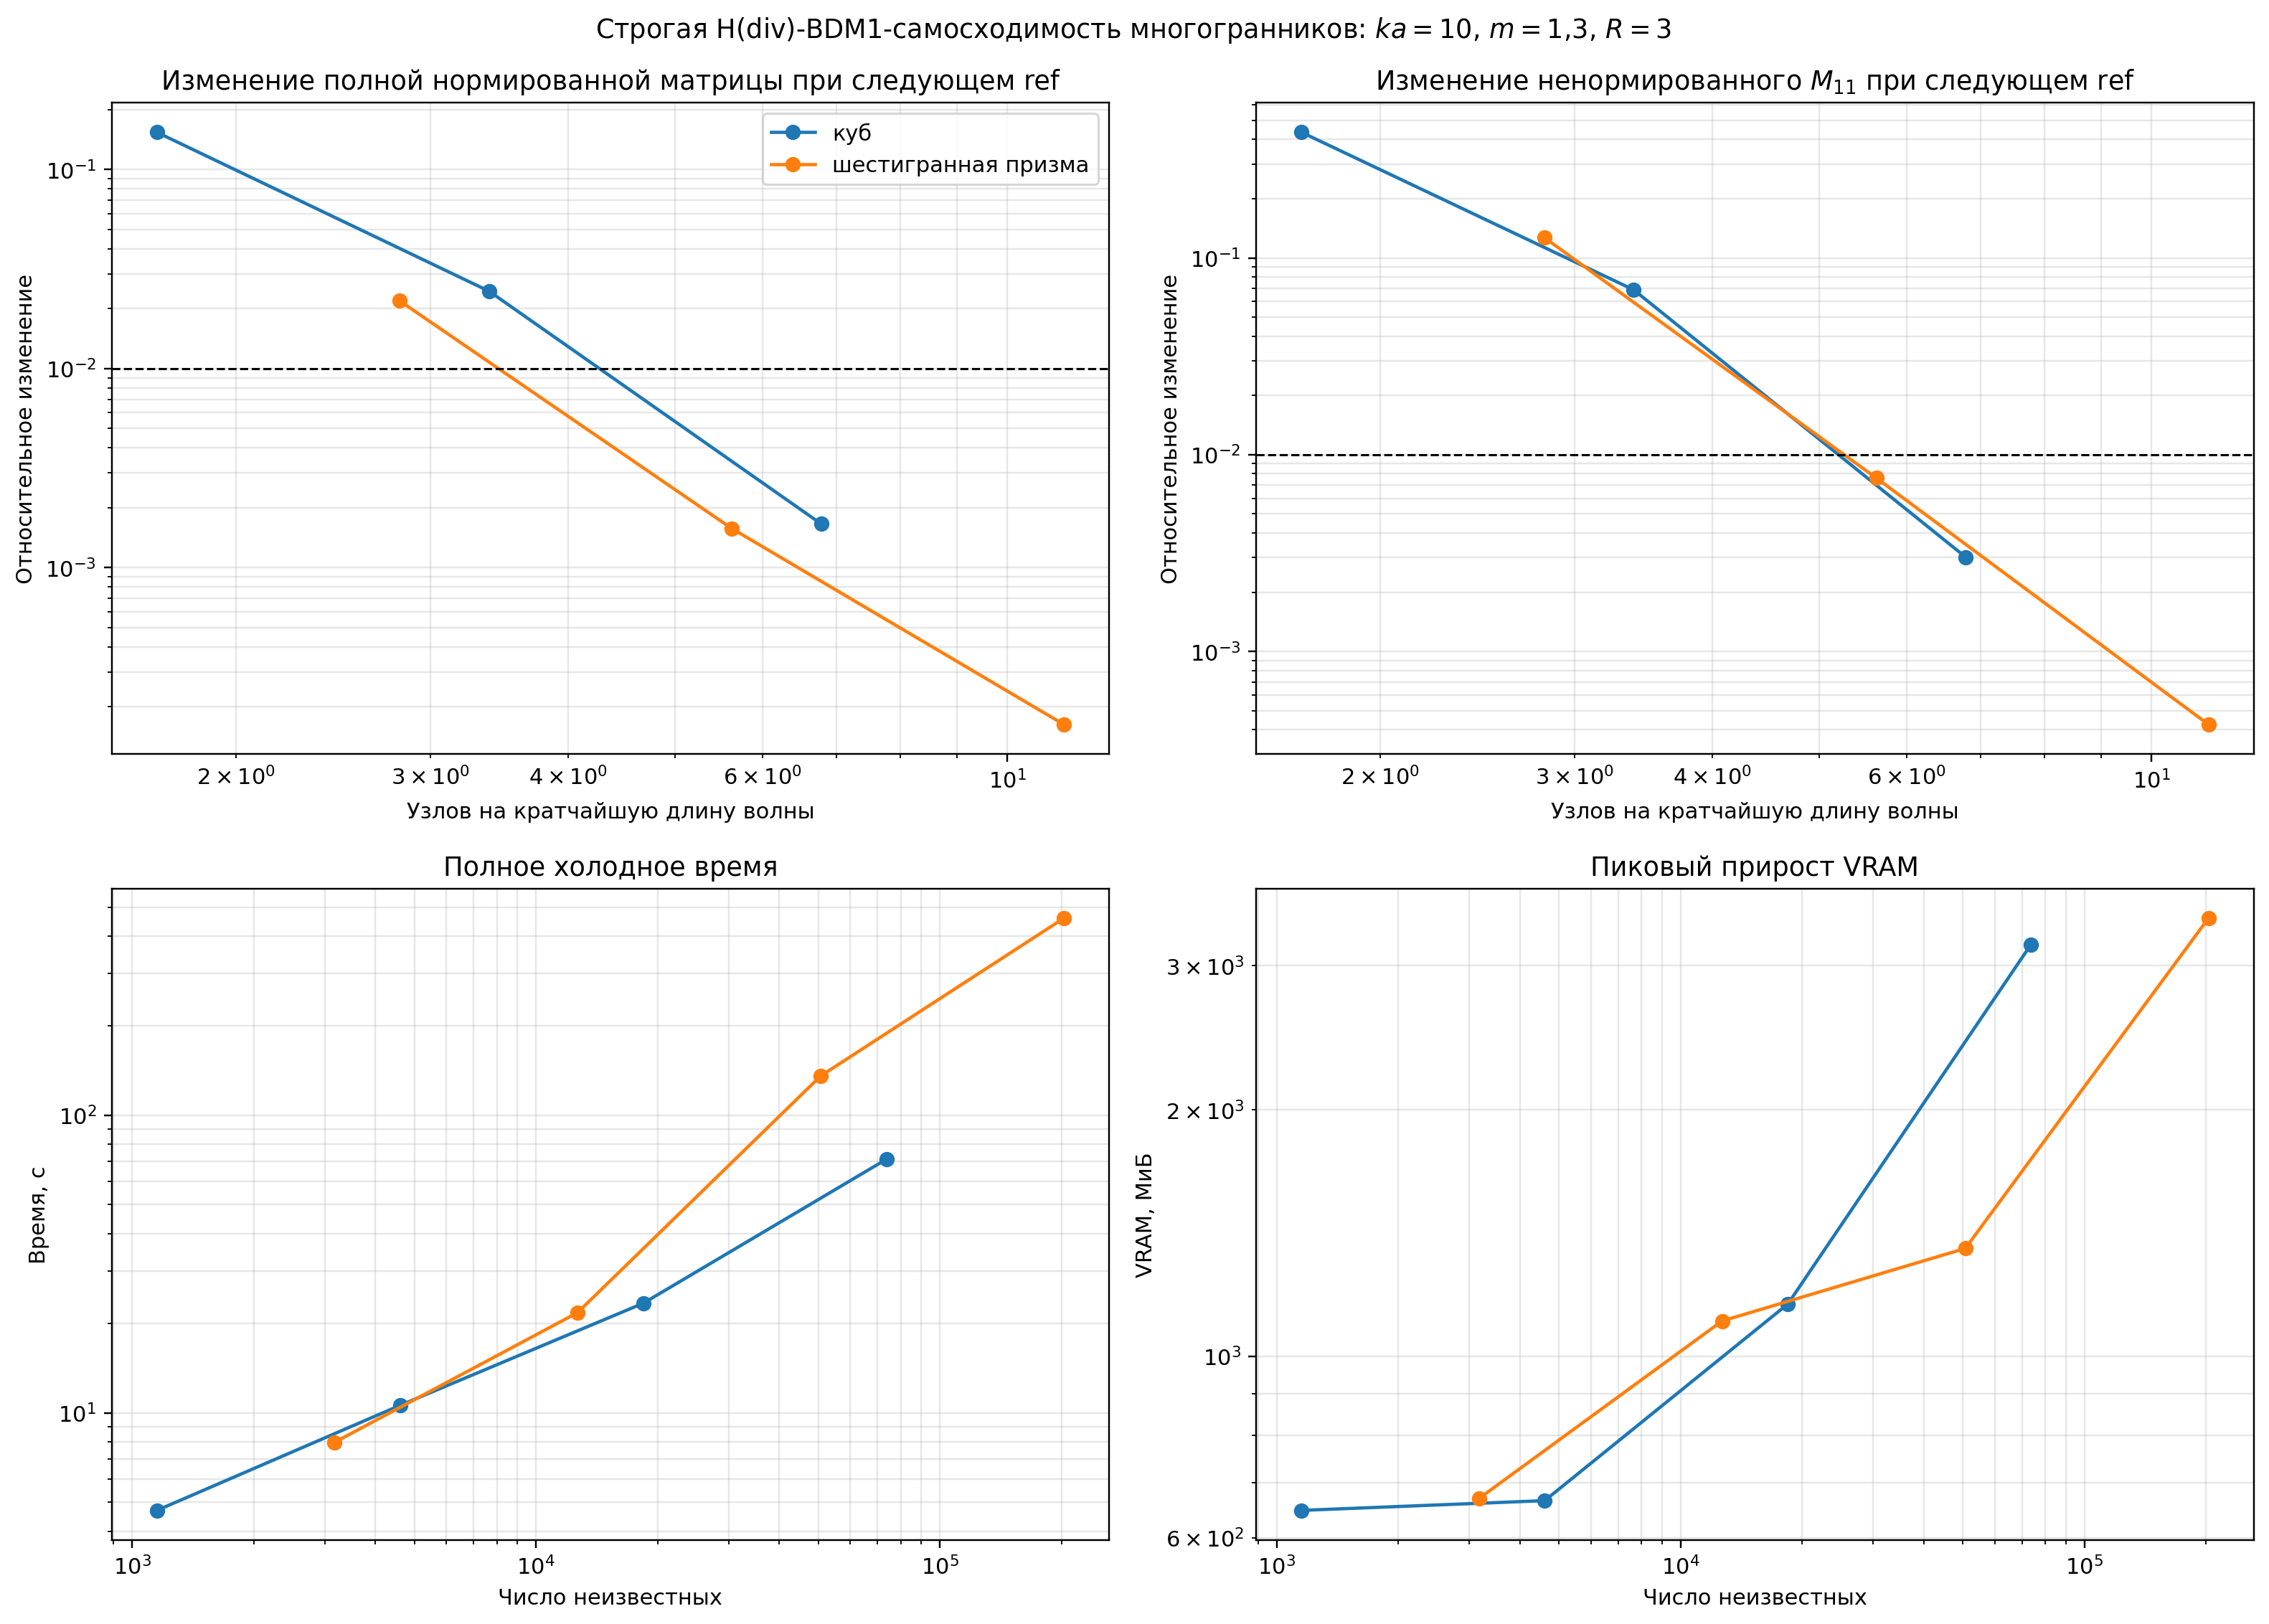
\includegraphics[width=0.98\textwidth]{mesh_polyhedra_hdiv_strict.png}
  \caption{Строгая H(div)-BDM1-самосходимость призмы и куба при $ka=10$,
  $m=1.3$ и $R=3$. Верхний ряд показывает изменение физического результата
  при следующем \texttt{ref}, нижний --- полное холодное время и VRAM.}
  \label{fig:strict-hdiv-polyhedra}
\end{figure}

\section{Вычислительные ресурсы и разложение времени}

\subsection{Что измеряется}

Каждый случай запускается через отдельный профилировщик. GNU \texttt{time -v}
даёт время процесса, CPU-время и максимальный RSS. Раз в заданный интервал
сохраняются RSS всего дерева процессов, число потоков, загрузка CPU, доступная
RAM, занятый swap, свободное место на файловой системе, загрузка GPU, занятая
VRAM, мощность, температура и частота SM. Интеграл мощности по времени даёт
энергию GPU. Версия Git, состояние рабочей копии, модель CPU/GPU, драйвер,
команда и переменные окружения записываются рядом с результатом.

CSV создаётся до запуска решателя, и каждая проба немедленно сбрасывается на
диск. При SIGINT или SIGTERM профилировщик пересылает сигнал всей группе
дочернего процесса, после чего агрегирует уже сохранённые пробы и записывает
номер сигнала. Поэтому контрольная точка решения и ресурсная история переживают
штатное прерывание независимо друг от друга.

Показания \texttt{nvidia-smi} относятся ко всей видеокарте, поэтому на время
случая берётся файловая блокировка GPU. Фоновый CUDA-процесс сделал бы VRAM,
загрузку и энергию невоспроизводимыми. Для коротких запусков мощность и энергия
являются только диагностическими: интервал опроса сравним с длительностью.

\subsection{Холодное и тёплое время}

Первый запуск включает
\begin{equation}
  T_{\mathrm{cold}}=T_{\mathrm{geom}}+T_{\mathrm{FMM}}+
  T_{\mathrm{near}}+T_{\mathrm{MBJ}}+T_{\mathrm{solve}}+
  T_{\mathrm{far}}+T_{\mathrm{I/O}}.
  \label{eq:cold-time}
\end{equation}
При неизменных геометрии, $ka$, $m$, базисе, квадратуре и операторе кэши
ближней коррекции и MBJ можно загрузить:
\begin{equation}
  T_{\mathrm{warm}}=T_{\mathrm{load}}+T_{\mathrm{solve}}+
  T_{\mathrm{far}}+T_{\mathrm{I/O}}.
  \label{eq:warm-time}
\end{equation}
Смешивать \eqref{eq:cold-time} и \eqref{eq:warm-time} в одном законе времени
нельзя. Для одного падения важен холодный расчёт, для усреднения по многим
ориентациям --- амортизированное тёплое время и стоимость решения каждой новой
правой части.

Runner адресует кэш двадцатизначным хешем содержимого оператора: в него входят
SHA-256 фактического бинарника и OBJ-файла, геометрия, $ka$, $m$, базис,
квадратура, FMM и MBJ. Имя экспериментальной серии, \texttt{setup-only},
допуск решателя и число выходных углов не входят, поскольку не меняют
кэшируемую систему. Поэтому прошедший барьер памяти без ручного копирования
подготавливает кэш последующему физическому случаю. Файловая блокировка
исключает одновременную запись в один кэш с нескольких GPU.
Для специального независимого измерения холодного старта параметр
\texttt{cache\_variant} в матрице эксперимента принудительно создаёт другой
хеш при неизменной физике.

\subsection{Ожидаемые законы масштабирования}

Из \eqref{eq:ref-scaling} число неизвестных примерно увеличивается в четыре
раза на уровень \texttt{ref}. Если бы порядок FMM и итерации были постоянны,
время действия было бы близко к линейному по $N$. В реальности
\begin{equation}
  T_{\mathrm{solve}}\approx
  n_{\mathrm{it}}(ka,m,h,P)
  \left[T_{\mathrm{near}}(N_q,R,B)+
  T_{\mathrm{far}}(N_q,p,L)+T_{\mathrm{proj}}(N,N_q)\right].
  \label{eq:time-model}
\end{equation}
Здесь $N_q$ --- число квадратурных источников, $R$ --- радиус ближней зоны,
$B$ --- лист, $p$ и $L$ заданы \eqref{eq:fmm-order}--\eqref{eq:fmm-directions}.
Поэтому показатель степени времени определяется регрессией только внутри
однородной серии с одинаковыми точностью, кэшем и алгоритмом.

Память также разлагается на геометрию и проекции $O(N+N_q)$, дерево и списки
пар, угловые коэффициенты порядка $O(N_{\mathrm{box}}L)$, ближнюю коррекцию,
MBJ-блоки и векторы Крылова. При перезапуске GMRES память базиса примерно
пропорциональна $N\,s$, где $s$ --- размер рестарта. Наибольший массив, а не
сумма размеров исходных данных, определяет достижимый \texttt{ref} на GPU.

Для квадратуры с $q$ точками на треугольник число глобальных источников
$N_q=qF$. Если MBJ делит $N_s$ скалярных узлов на блоки ядра длины $b$ и
добавляет по $o$ узлов перекрытия с каждой стороны Morton-порядка, размер
локальной матрицы не превосходит $n_b=4(b+2o)$. Поэтому оценки хранения LU и
работы её построения имеют вид
\begin{equation}
  S_{\mathrm{MBJ}}=O\!\left(\frac{N_s}{b}\,[4(b+2o)]^2\right),\qquad
  T_{\mathrm{MBJ}}=O\!\left(\frac{N_s}{b}\,[4(b+2o)]^3\right).
  \label{eq:mbj-resource-model}
\end{equation}
Это верхние структурные оценки, а не предсказания секунд: граничные блоки
короче, кэширование меняет холодное время, а GPU-FMM и CPU-факторизация имеют
разные коэффициенты стоимости. Для GMRES с рестартом $s$ только два набора
комплексных векторов Крылова уже дают величину порядка $2Ns$ чисел, поэтому
увеличение $s$ должно сопровождаться прямым измерением VRAM/RSS.

\subsection{Точность хранения и вычислений}

Исполняемый файл \texttt{muller\_nodal\_fmm\_demo} является строгим FP64
контролем там, где реализация предоставляет двойную точность. Вариант с
суффиксом \texttt{\_fp32} использует FP32 для части ближних CUDA-ядер,
плосковолновых фаз и отдельных FMM-накоплений, но оставляет коэффициенты
Крылова, MBJ, итоговую сборку и проверку невязки в FP64. Поэтому это смешанная,
а не полностью одинарная точность.

Флаг \texttt{--fmm-near-fp32} меняет арифметику большого числа прямых пар и
должен проверяться сравнением с \texttt{--fmm-near-fp64} на одинаковой сетке.
Выбор точности не выполняется по одной малой невязке: сравниваются действие
оператора, токи и вся матрица Мюллера. В основной сеточной серии используется
FP64, а производственная ресурсная серия отдельно измеряет смешанный путь.

\subsection{Угловая сетка и ориентационное усреднение}

Параметр \texttt{ntheta} определяет число выходных углов рассеяния и почти не
влияет на решение линейной системы; он меняет стоимость дальнего поля и
точность последующего углового интеграла. В данной серии 181 точка с шагом
$1^\circ$ является выбранной сеткой вывода, но её достаточность проверяется
отдельным сгущением углов, а не поверхностным \texttt{ref}.

Тройка \texttt{--orient-average $N_\alpha$ $N_\beta$ $N_\gamma$} задаёт число
узлов по углам Эйлера. Вращение на $\alpha$ вокруг направления падающей волны
может быть обработано повторным вычислением дальнего поля из тех же токов;
изменения $\beta,\gamma$ обычно создают новые правые части. Адаптивный режим
увеличивает вложенные сетки до выполнения трёх критериев: формы $M_{11}$, её
интеграла и нормированных компонентов. Параметр симметрии разрешено применять
только после проверки геометрического отображения и коммутатора дискретного
оператора. Симметрия сокращает число правых частей, но не улучшает точность
одной поверхностной сетки.

\section{План факторного вычислительного эксперимента}

Полная матрица находится в файле \texttt{study\_config.json}; после
адаптивного исключения сеток, уже не способных изменить вывод, она содержит
169 воспроизводимых запусков. Серии имеют следующий смысл:
\small
\begin{longtable}{>{\raggedright\arraybackslash}p{0.30\textwidth}p{0.61\textwidth}}
\toprule
Серия & Что изменяется и что фиксируется \\
\midrule
\endfirsthead
\toprule
Серия & Что изменяется и что фиксируется \\
\midrule
\endhead
\texttt{calibration} & Холодный/тёплый кэш, FP64/смешанная точность и повторяемость при одной малой задаче.\\
\texttt{mesh\_sphere\_m13} & $ka=2,5,10,20,40,60$ и последовательные \texttt{ref}; $m=1.3$, строгие FMM и квадратура, эталон Ми.\\
\texttt{mesh\_sphere\_contrast} & Несколько $m$ при фиксированных $ka$ и последовательных сетках; проверка свёртки по $P_{\min}$.\\
\texttt{mesh\_prism} & Самосходимость шестигранной призмы в H(div)-BDM1.\\
\texttt{mesh\_\allowbreak polyhedra\_\allowbreak hdiv\_\allowbreak strict} & Строгая H(div)-BDM1-самосходимость призмы и куба на \texttt{ref}=2,\ldots,5 при $R=3$.\\
\texttt{basis\_edge\_control} & Сравнение smooth/split/H(div) на одной острой геометрии.\\
\texttt{fmm\_digits} & Фактические $d=3,\ldots,7$ при фиксированном радиусе и листе.\\
\texttt{fmm\_near\_radius} & $R=1,\ldots,6$ при фиксированных $d$ и листе.\\
\texttt{fmm\_leaf} & Лист 32, 64, 128, 256 при фиксированных $d$ и $R$.\\
\texttt{fmm\_radius\_scale} & Повтор радиусной серии при нескольких $ka$; проверка переносимости вывода.\\
\texttt{fmm\_radius\_digits\_grid} & Полная сетка $R=1,3,5$ и $d=3,5,7$; совместная граница точность--время--память.\\
\texttt{fmm\_radius\_dependency} & Перенос радиусной серии на $m=2$ и острую H(div)-призму.\\
\texttt{solver\_controls} & Рестарт GMRES, размер и перекрытие блоков MBJ, алгебраический допуск при одной разрешённой сфере; по два повтора.\\
\texttt{farfield\_grid} & 37, 73, 181 и 361 выходной угол; отделение стоимости и точности углового интегрирования от \texttt{ref}.\\
\texttt{quadrature} & Обычная квадратура 4/7/13 и Даффи 4/6/8 по одному фактору.\\
\texttt{resource\_scaling} & По три повтора холодного и тёплого режима для $ka=5,10,20,30,40$; совместное измерение времени, RAM, VRAM и энергии.\\
\texttt{memory\_gates} & Только построение крупнейших операторов перед расходующим часы решением.\\
\bottomrule
\end{longtable}
\normalsize

Текущий вычислительный статус не редактируется вручную, а пересчитывается из
машиночитаемых файлов каждого запуска:
\begin{table}[H]
\centering
\caption{Состояние матрицы экспериментов на момент сборки этого PDF. ``Принято''
означает успешное прохождение автоматической проверки результата; ошибка и
незавершённый случай не подменяются отсутствующим значением.}
\resizebox{0.92\textwidth}{!}{%
\begin{tabular}{lrrrr}
\toprule
Серия & План & Принято & Ошибка & Осталось\\
\midrule
\texttt{calibration} & 4 & 4 & 0 & 0\\
\texttt{mesh\_sphere\_m13} & 22 & 22 & 0 & 0\\
\texttt{mesh\_sphere\_contrast} & 14 & 14 & 0 & 0\\
\texttt{mesh\_prism} & 14 & 14 & 0 & 0\\
\texttt{mesh\_polyhedra\_hdiv\_strict} & 8 & 8 & 0 & 0\\
\texttt{basis\_edge\_control} & 8 & 8 & 0 & 0\\
\texttt{fmm\_digits} & 5 & 5 & 0 & 0\\
\texttt{fmm\_near\_radius} & 6 & 6 & 0 & 0\\
\texttt{fmm\_leaf} & 4 & 4 & 0 & 0\\
\texttt{fmm\_shared\_cold\_audit} & 1 & 1 & 0 & 0\\
\texttt{fmm\_radius\_scale} & 8 & 8 & 0 & 0\\
\texttt{fmm\_radius\_digits\_grid} & 9 & 9 & 0 & 0\\
\texttt{fmm\_radius\_dependency} & 6 & 6 & 0 & 0\\
\texttt{fmm\_radius\_cold\_audit} & 1 & 1 & 0 & 0\\
\texttt{solver\_controls} & 26 & 26 & 0 & 0\\
\texttt{farfield\_grid} & 4 & 4 & 0 & 0\\
\texttt{quadrature} & 18 & 18 & 0 & 0\\
\texttt{resource\_scaling} & 15 & 15 & 0 & 0\\
\texttt{memory\_gates} & 4 & 4 & 0 & 0\\
\bottomrule
\end{tabular}

}
\label{tab:study-progress}
\end{table}

Основная строгая конфигурация: FP64-путь, ближняя часть FP64, квадратура 13,
Даффи 6, запрошенные и разрешённые \texttt{digits}=7, лист 64, радиус 5,
истинная невязка $2\cdot10^{-6}$, максимум 2000 итераций, 181 угол. Эти
параметры намеренно дороже производственного режима: в сеточной серии ошибка
оператора должна быть меньше исследуемой ошибки сетки. Для крупных точек
$ka=40,60$ после отдельной абсолютной проверки применяется $R=3$ и допуск
$10^{-4}$: при $ka=40$ этот радиус воспроизводит решение Ми с ошибкой менее
0.08\%, тогда как $R=1,2$ не проходят физический контроль. В двух
высококонтрастных точках $ka=40$ использован допуск $10^{-3}$: он на порядок
строже физического бюджета 1\%, а каждая принятая поляризация дополнительно
проверена непосредственным действием полного FMM-оператора.

\section{Первые результаты}

\subsection{Сходимость сферы при $m=1.3$}

На рис.~\ref{fig:mie-ppw} приведены все точки завершённого адаптивного плана;
исключённые более тонкие сетки не подменяются нулевой ошибкой.
\begin{figure}[H]
  \centering
  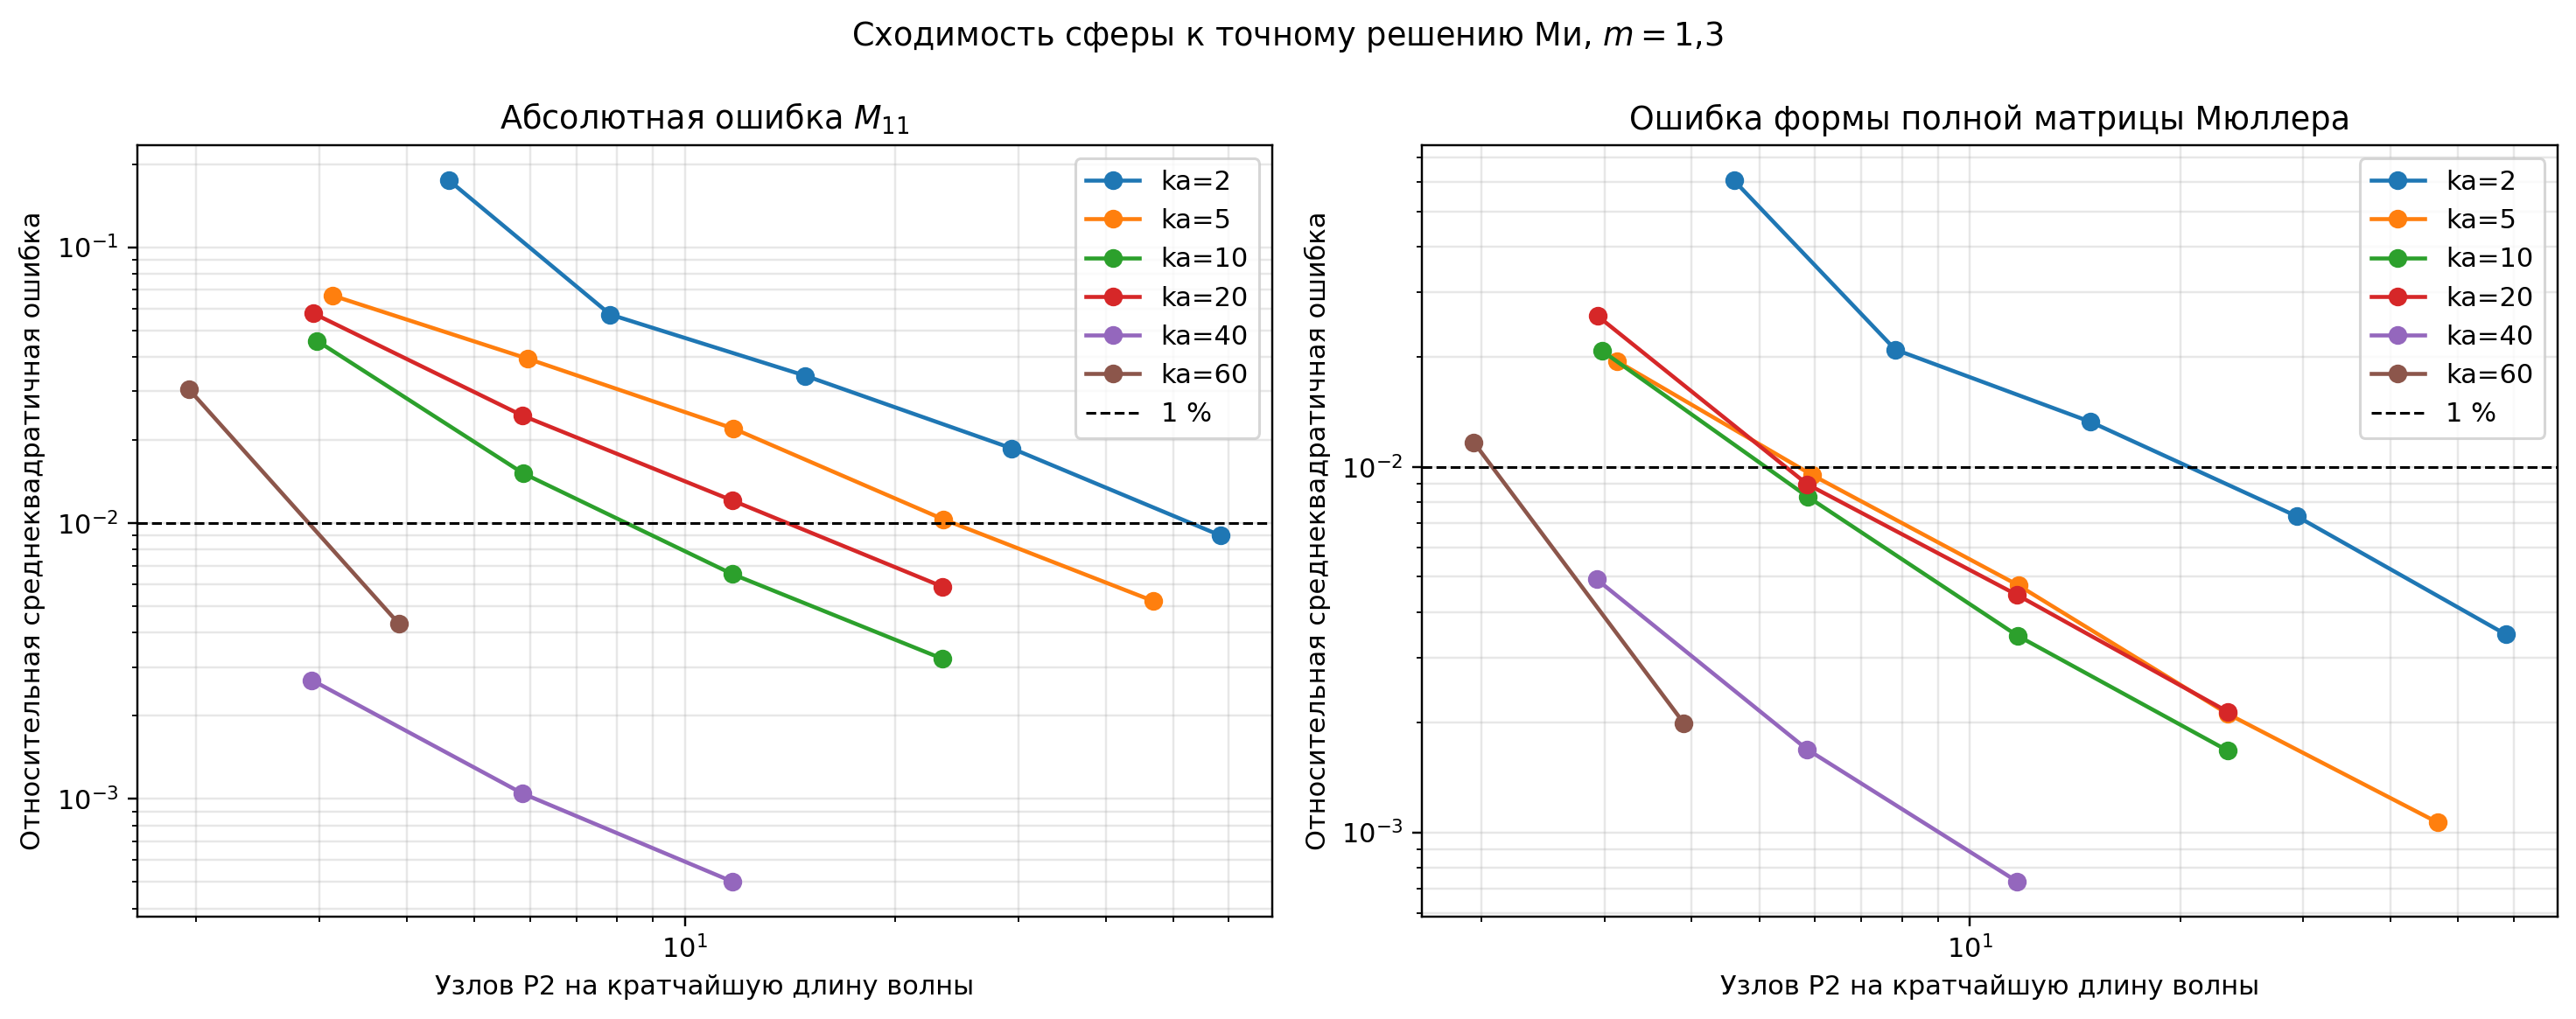
\includegraphics[width=0.98\textwidth]{mesh_mie_error_vs_ppw.png}
  \caption{Сходимость сферы к точному решению Ми. Слева сохранён абсолютный
  масштаб $M_{11}$, справа сравнивается форма полной матрицы после нормировки.}
  \label{fig:mie-ppw}
\end{figure}

\begin{table}[H]
\centering
\caption{Минимальные завершённые сетки, на которых пять физических критериев
не превышают 1\%. ``Кандидат'' означает отсутствие следующей более тонкой
точки; ``подтверждён'' означает, что следующее сгущение также изменило
результат менее чем на 1\%.}
\resizebox{\textwidth}{!}{%
\begin{tabular}{rrrrrrl}
\toprule
$ka$ & \texttt{ref} & $P_{\min}$ & $N$ & $E_{11}^{\rm raw}$ & $E_{\rm full}$ & статус\\
\midrule
2 & 4 & 58.51 & 40968 & 0.899\% & 0.348\% & точный эталон Ми\\
5 & 5 & 46.77 & 163848 & 0.522\% & 0.106\% & точный эталон Ми\\
10 & 4 & 11.70 & 40968 & 0.652\% & 0.345\% & Ми + соседняя сетка\\
20 & 6 & 23.38 & 655368 & 0.588\% & 0.214\% & точный эталон Ми\\
40 & 4 & 2.93 & 40968 & 0.269\% & 0.492\% & Ми + соседняя сетка\\
60 & 5 & 3.90 & 163848 & 0.431\% & 0.199\% & точный эталон Ми\\
\bottomrule
\end{tabular}

}
\label{tab:mesh-first}
\end{table}

Для $ka=40$ выполнена отдельная последовательность с уже проверенным радиусом
$R=3$. На \texttt{ref}=4 система содержит 40~968 неизвестных, обе поляризации
сходятся за $99+98$ итераций, а холодный процесс занимает 365.4~с. Ошибки
$M_{11}$, полной нормированной матрицы, направления вперёд, интеграла и
максимального нормированного элемента равны соответственно 0.269, 0.492,
0.145, 0.579 и 0.190\%. На \texttt{ref}=5 при 163~848 неизвестных время
возрастает до 1107.6~с, а эти ошибки уменьшаются до 0.105, 0.169, 0.093,
0.094 и 0.062\%. Уже рассчитанная \texttt{ref}=6 даёт 655~368 неизвестных и
ошибки 0.050, 0.073, 0.037, 0.037 и 0.030\%. Изменение полной нормированной
матрицы при переходах $4\to5$ и $5\to6$ равно 0.342 и 0.0995\%.
Следовательно, для бюджета 1\% минимально подтверждена \texttt{ref}=4, а
расчёт \texttt{ref}=7 не требуется: он не способен изменить уже сделанный
вывод, но потребовал бы существенно больше памяти и времени.

При $ka=60$ грубая сетка \texttt{ref}=4 содержит те же 40~968 неизвестных,
что и при $ka=40$, но только 1.95 узла P2 на кратчайшую внутреннюю волну. Она
не проходит критерий: ошибка $M_{11}$ равна 3.06\%, полная нормированная
ошибка --- 1.17\%, ошибка вперёд --- 3.44\%, интегральная --- 4.20\%.
Расчёт занял 339.7~с и 3.69~ГиБ VRAM. На \texttt{ref}=5 число узлов на
кратчайшую волну возрастает до 3.90, а соответствующие ошибки уменьшаются до
0.431, 0.199, 0.396 и 0.528\%; максимальное абсолютное отличие
нормированных элементов равно 0.106\%. Полное время составляет 2022.8~с,
пик VRAM --- 7.41~ГиБ, обе поляризации требуют 172 и 174 итерации.
Таким образом, точное решение Ми подтверждает \texttt{ref}=5 как минимальную
проверенную сетку для этой точки. Отдельная setup-only проверка
\texttt{ref}=6 показала, что сборка занимает 472.8~с, пик VRAM равен
9.35~ГиБ, а RSS --- около 7.54~ГиБ; полный многчасовой расчёт не требуется
для решения уже закрытого вопроса о сетке с бюджетом 1\%.

Табл.~\ref{tab:mesh-first} опровергает слишком простое правило ``одинаковое
$P_{\min}$ даёт одинаковую ошибку''. При $ka=2$ относительная ошибка масштаба
остаётся 1.87\% даже при $P_{\min}=29.36$, тогда как при $ka=10$ значение
$P_{\min}=11.70$ уже даёт 0.652\%. На малой сфере абсолютная ошибка сильнее
чувствительна к аппроксимации кривизны икосаэдрической геометрией и к масштабу
рассеяния. При большем $ka$ начинает доминировать волновое разрешение. Поэтому
автоматическое правило должно содержать два ограничения:
\begin{equation}
  r\ge \max\{r_{\mathrm{geometry}}(\Gamma,\epsilon),
  r_{\mathrm{wave}}(ka,m,P_*)\}.
  \label{eq:two-grid-criteria}
\end{equation}

\begin{figure}[H]
  \centering
  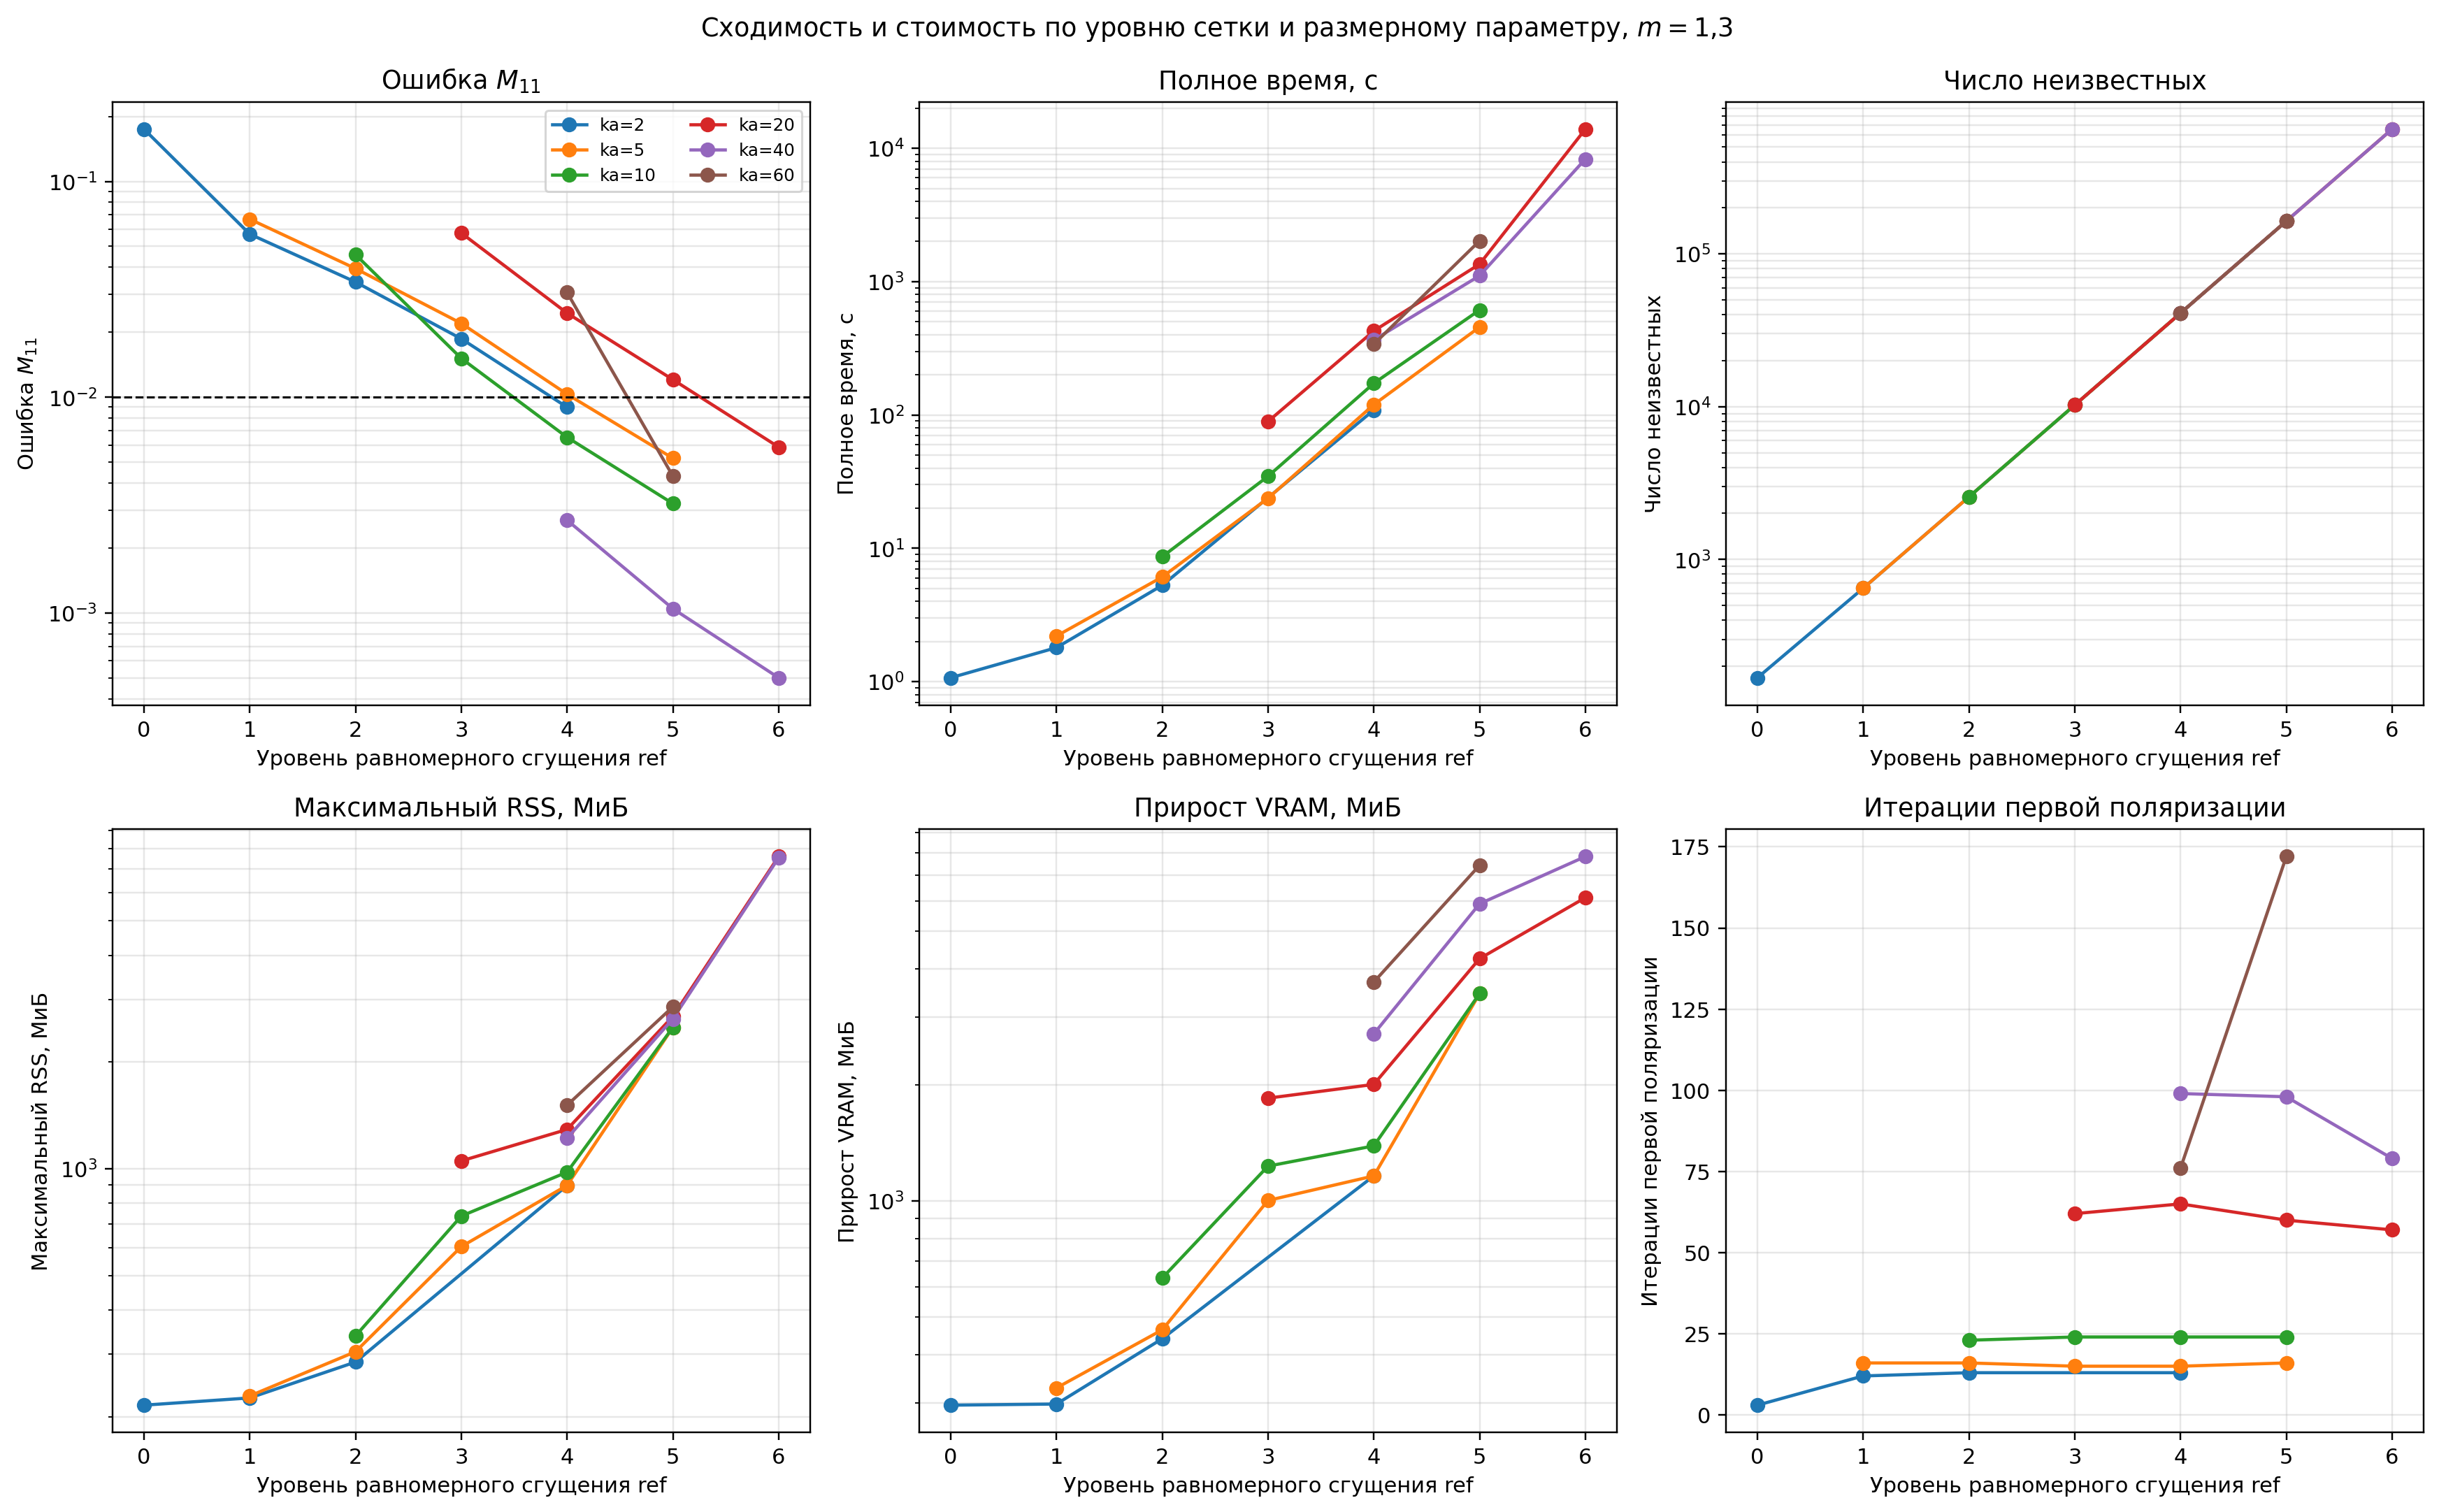
\includegraphics[width=\textwidth]{mesh_ref_ka_scaling.png}
  \caption{Одновременное изменение ошибки, времени, числа неизвестных, RAM,
  VRAM и итераций по \texttt{ref}. Возобновлённые после прерванного строгого
  запуска точки используются для физики, но исключены из чистой регрессии
  производительности.}
  \label{fig:ref-scaling}
\end{figure}

Увеличение \texttt{ref} на единицу точно увеличивает $N$ примерно в четыре
раза, но время не обязано расти в четыре раза: меняются глубина дерева, порядок
разложения, доля прямой ближней работы и число итераций. Это видно особенно при
сравнении разных $ka$ на одном $N$.

Для количественной, но пока описательной оценки выполнена регрессия
\begin{equation}
  y=C\,N^{\alpha_N}(ka)^{\beta_{ka}}
  \label{eq:empirical-resource-model}
\end{equation}
по холодным невозобновлённым точкам FP64-сферы при $m=1.3$:
\begin{table}[H]
\centering
\caption{Текущие коэффициенты модели \eqref{eq:empirical-resource-model}.
Это аппроксимация измеренного диапазона, а не теорема о сложности FMM.}
\resizebox{0.9\textwidth}{!}{%
\begin{tabular}{lrrrrr}
\toprule
Отклик $y$ & $n$ & $C$ & $\alpha_N$ & $\beta_{ka}$ & $R^2$\\
\midrule
полное время, с & 22 & 0.00158 & 1.013 & 0.443 & 0.975\\
RSS, МиБ & 22 & 12.2 & 0.415 & 0.125 & 0.940\\
прирост VRAM, МиБ & 22 & 25.3 & 0.338 & 0.331 & 0.962\\
\bottomrule
\end{tabular}

}
\end{table}
Доверительные интервалы коэффициентов и число степеней свободы сохраняются в
\texttt{generated/resource\_models.json}. Значения будут автоматически
пересчитаны после новых $ka$ и \texttt{ref}. Корреляция $N$, порядка дерева и
числа итераций не позволяет интерпретировать $\alpha_N$ как чистую
алгоритмическую степень; для этого дополнительно приводятся локальные отношения
соседних сеток в \texttt{generated/local\_scaling.csv}.

\begin{figure}[H]
  \centering
  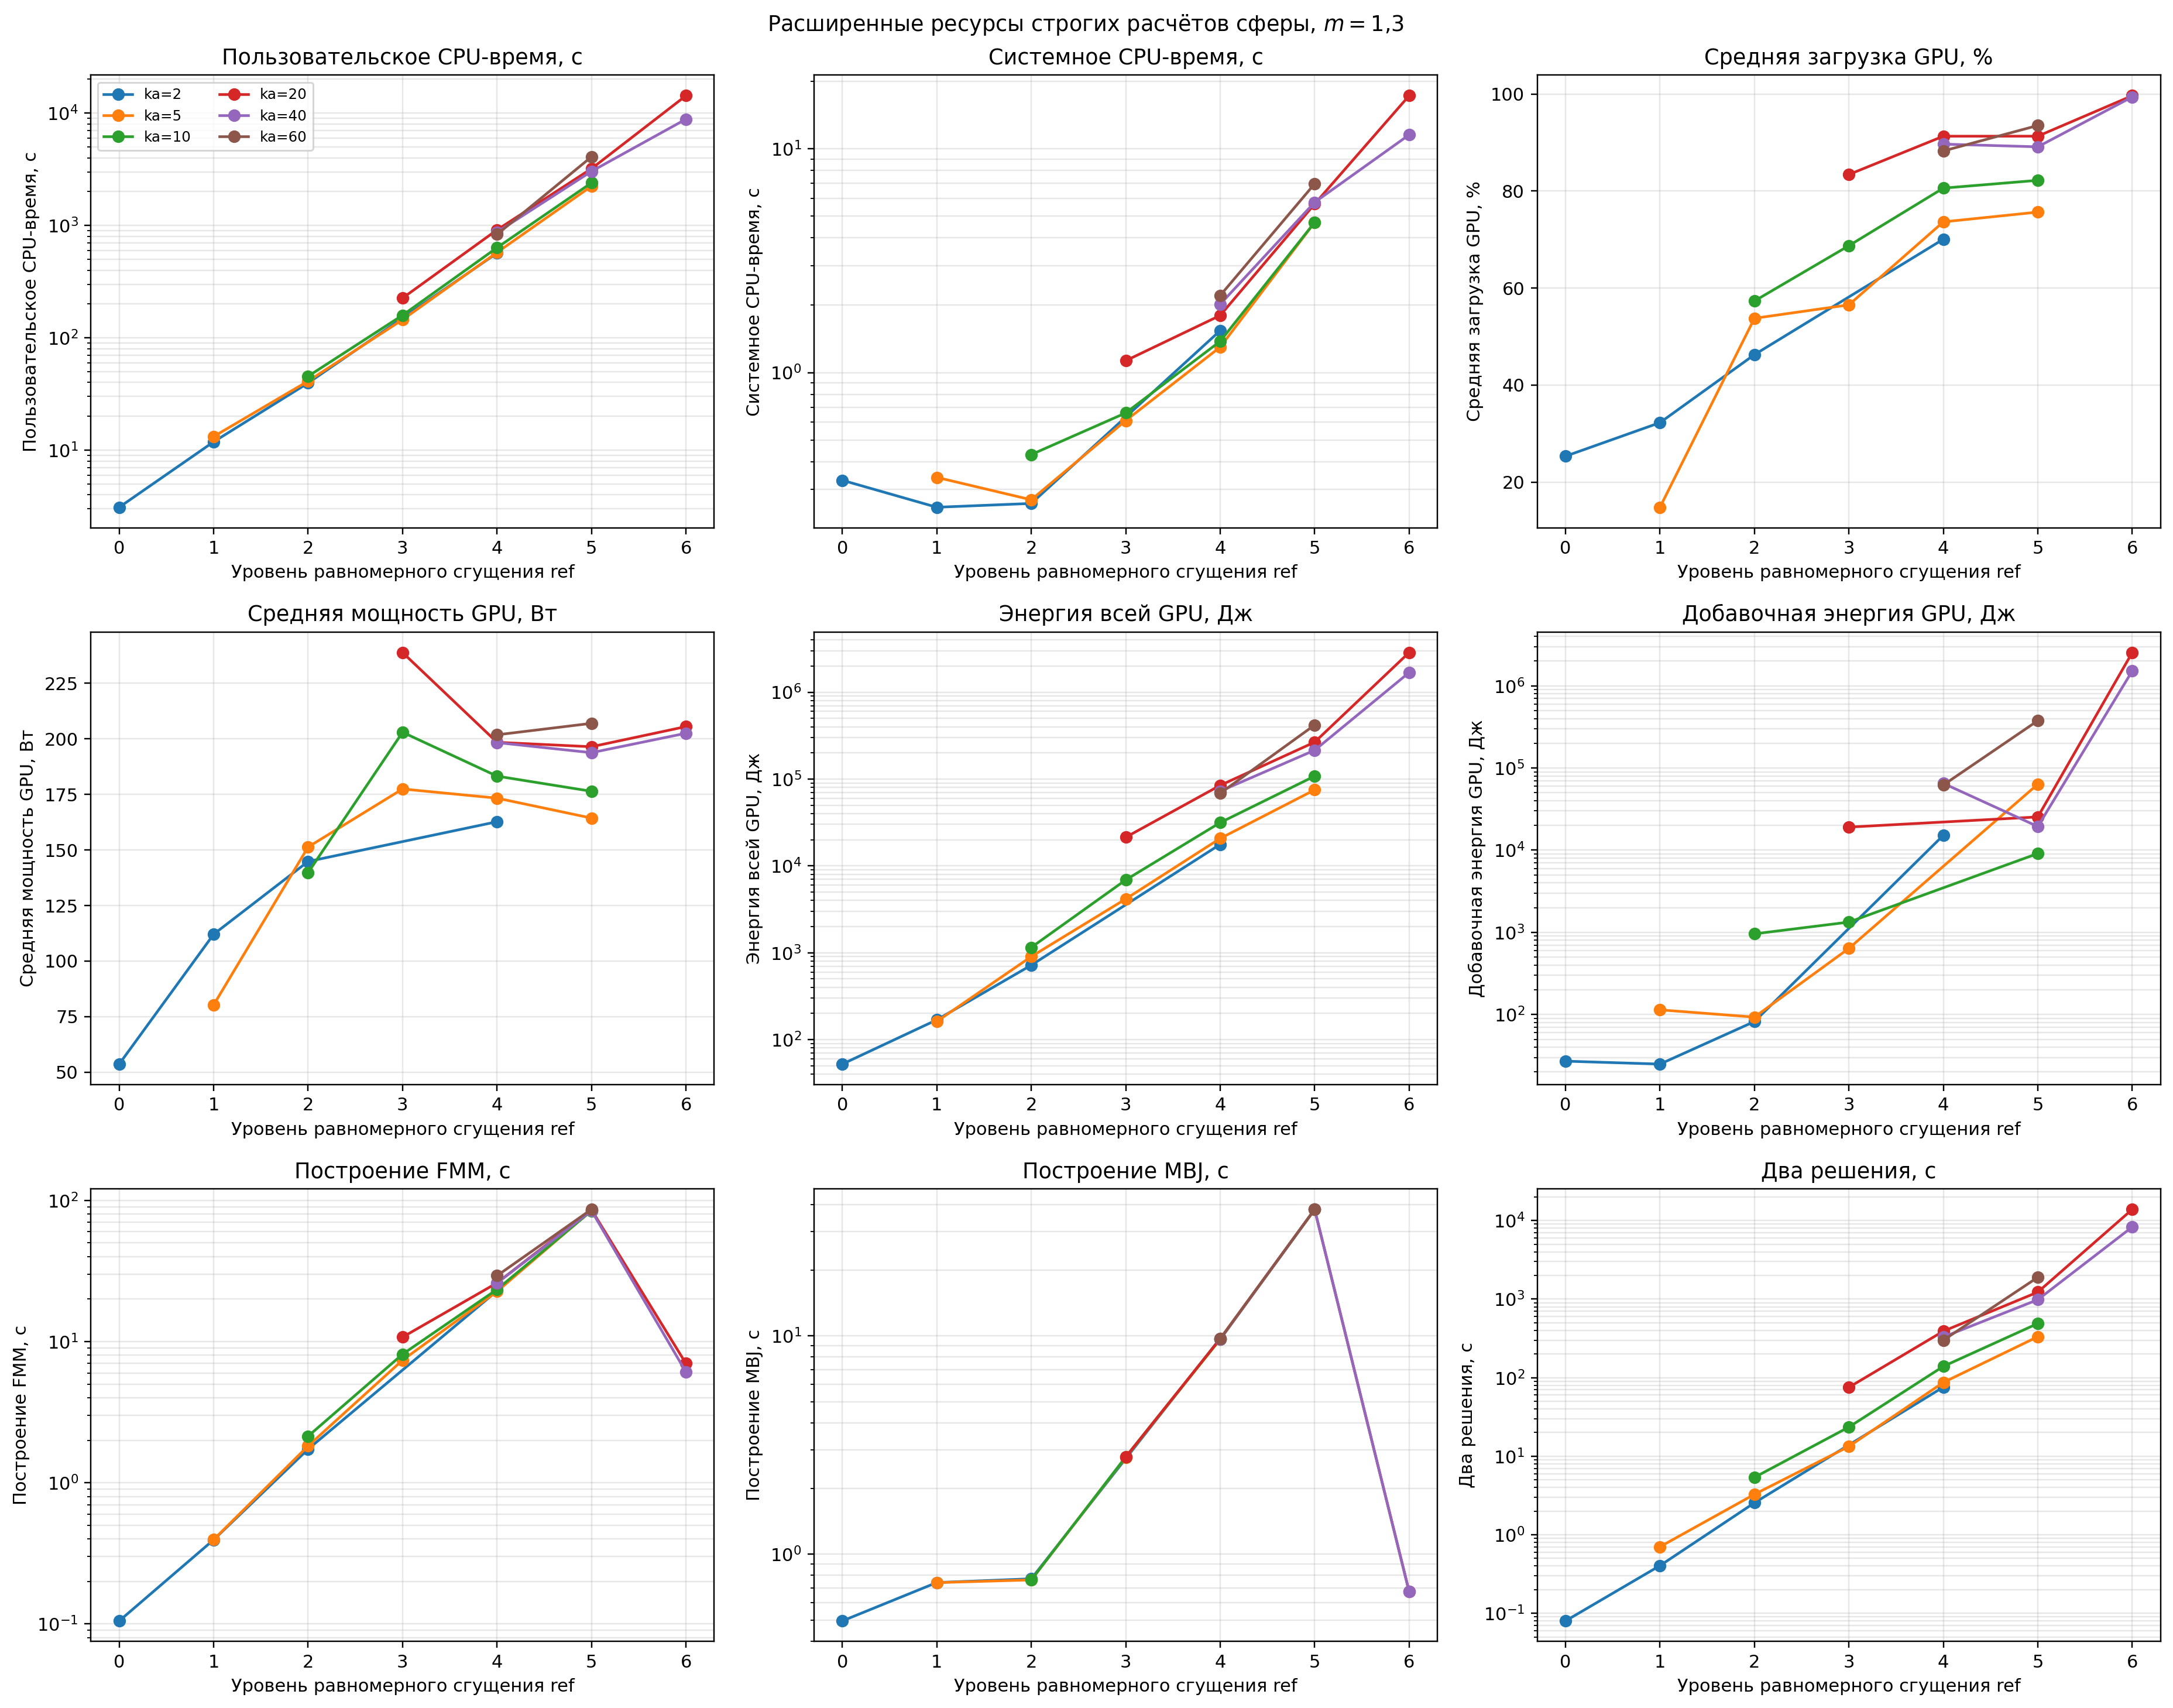
\includegraphics[width=\textwidth]{mesh_ref_ka_extended_resources.png}
  \caption{Расширенные ресурсные показатели: CPU-время, загрузка, мощность и
  энергия GPU, а также внутренние времена построения FMM, MBJ и двух решений.
  Энергия коротких случаев является диагностической из-за интервала опроса.}
  \label{fig:extended-resources}
\end{figure}

\begin{figure}[H]
  \centering
  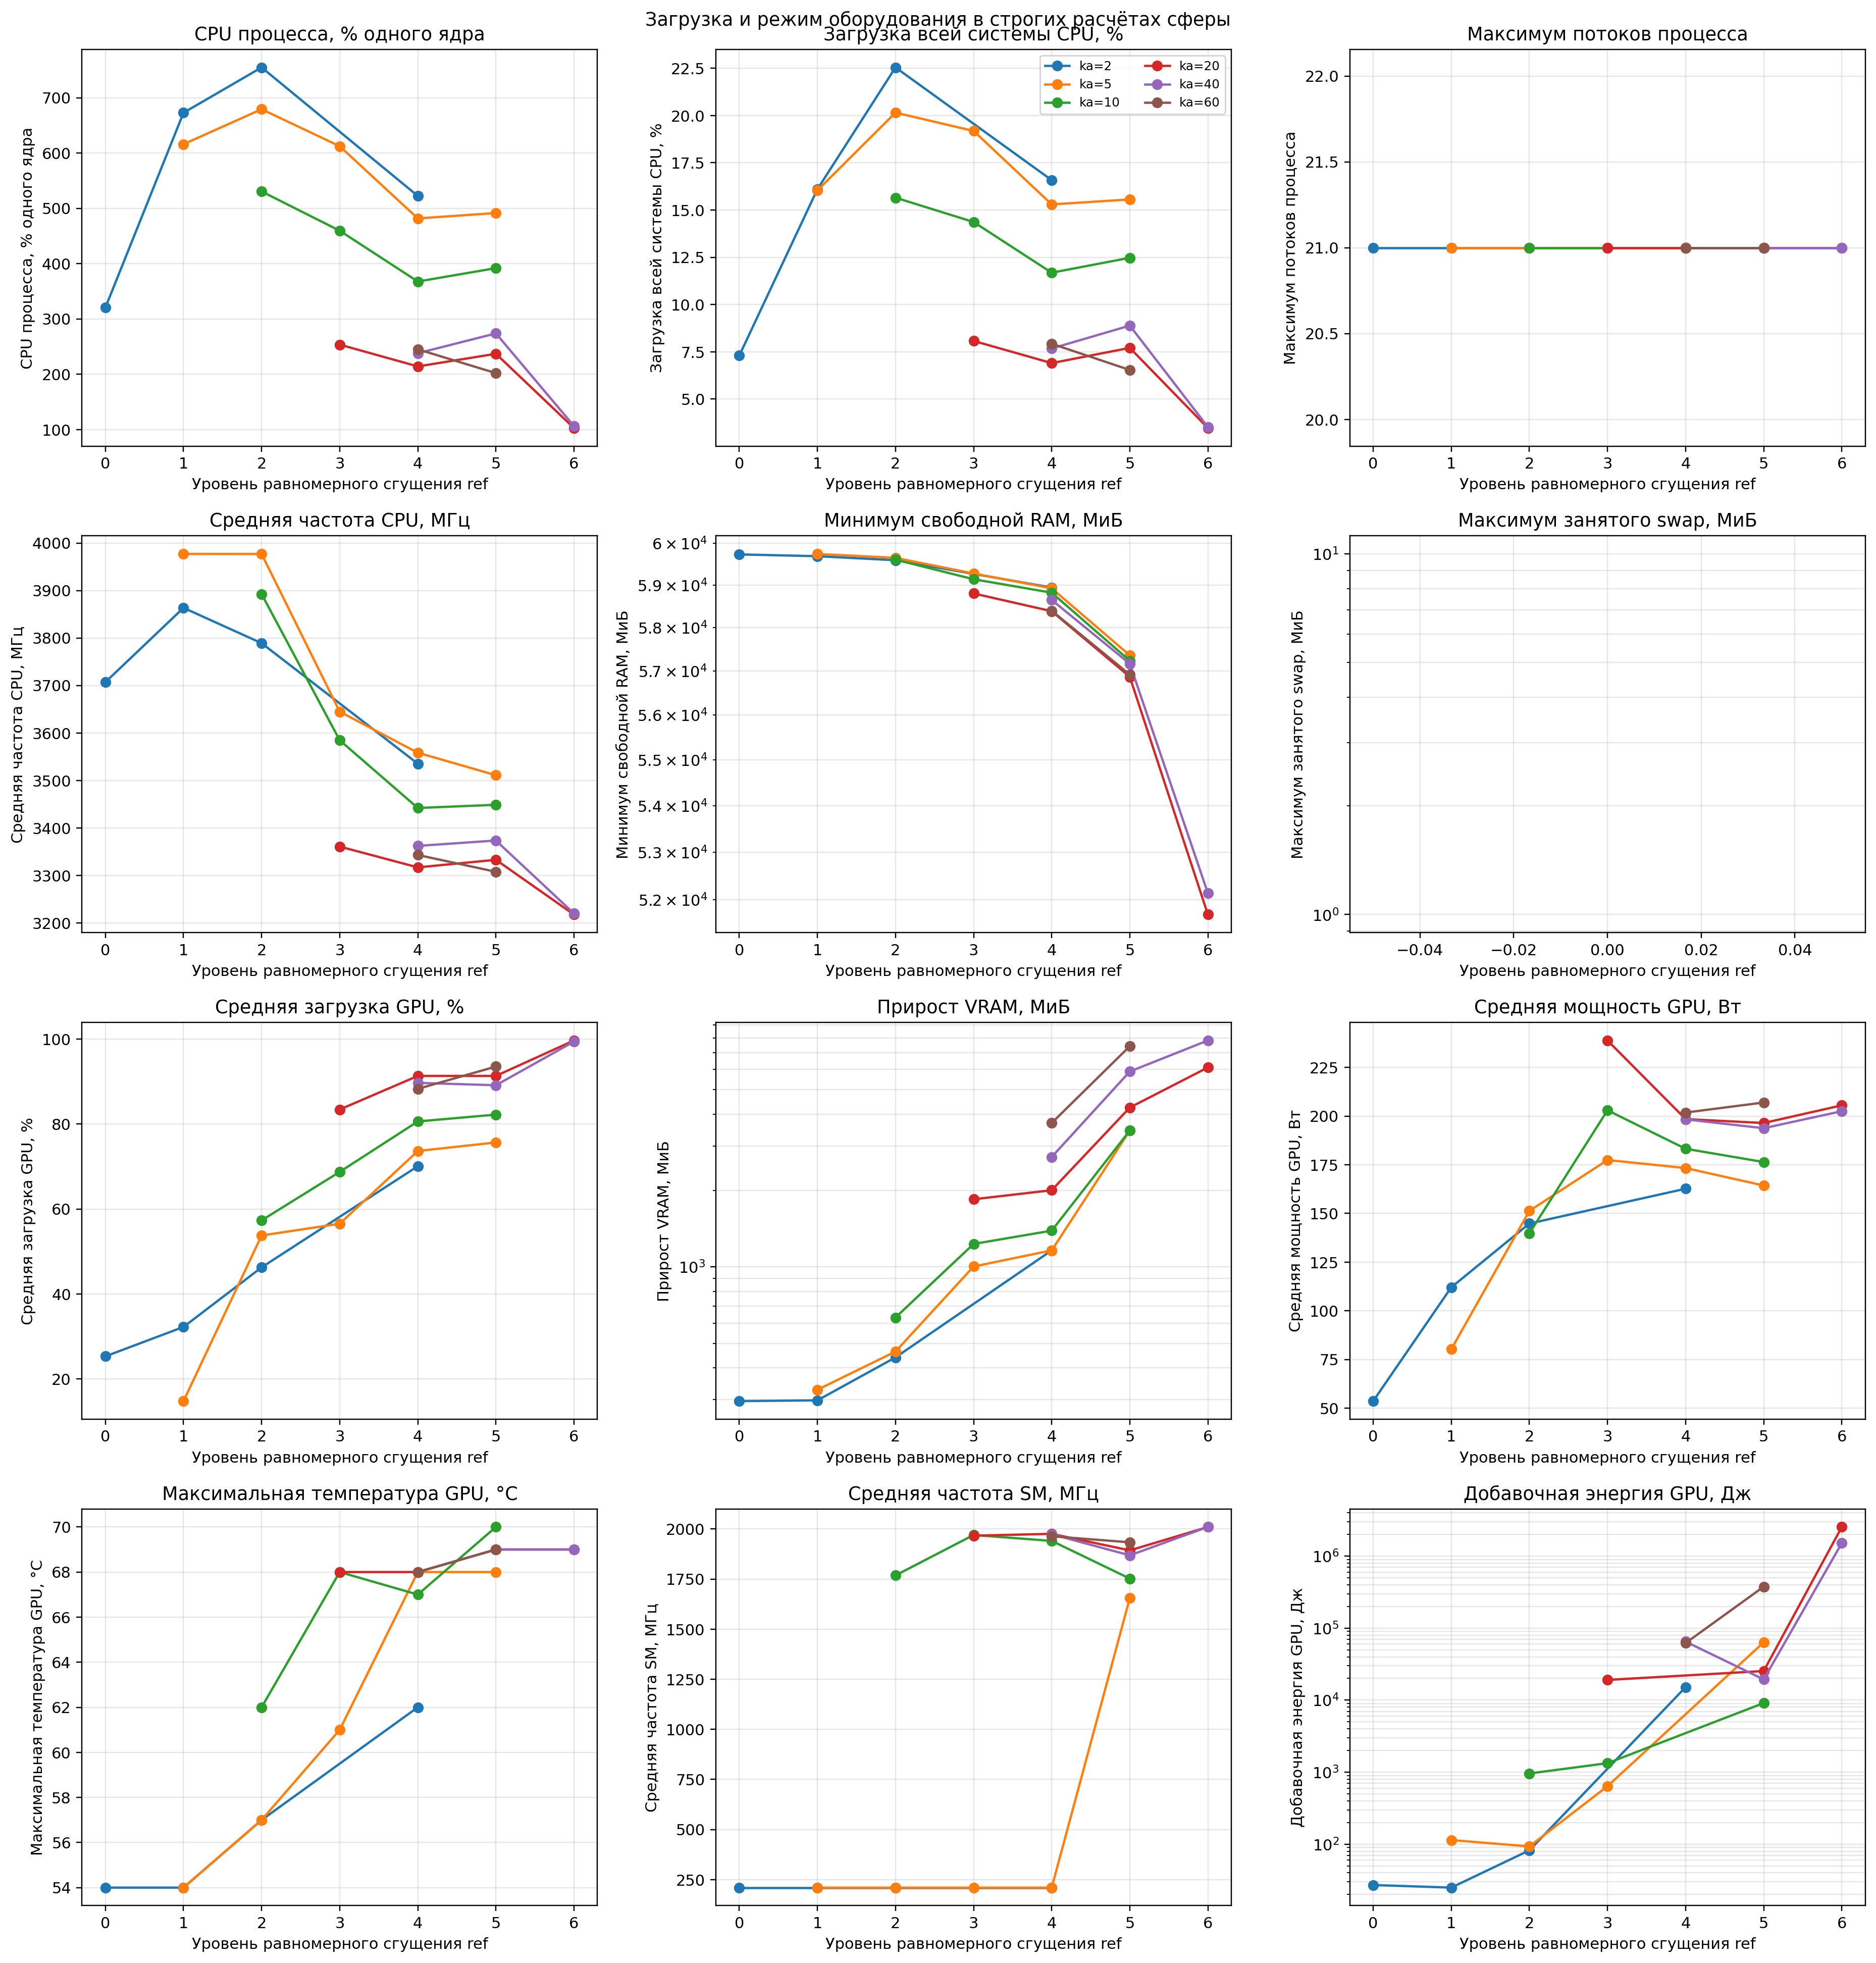
\includegraphics[width=\textwidth]{mesh_ref_ka_hardware_utilization.png}
  \caption{Режим оборудования во время тех же строгих расчётов: загрузка и
  частота CPU, загрузка, мощность, температура, частота и энергия GPU.
  Для загрузки процесса 100\% означает одно полностью занятое логическое ядро,
  поэтому многопоточное значение может превышать 100\%. В старых профилях оно
  восстановлено точно по сумме пользовательского и системного CPU-времени,
  делённой на стеночное время; новые профили дополнительно содержат прямой
  временной ряд.}
  \label{fig:hardware-utilization}
\end{figure}

Загрузка GPU, мощность и полезная пропускная способность не являются одной
величиной. FMM чередует нерегулярные обращения к памяти, короткие ядра
проекций, M2L/P2P и синхронизации. Поэтому значение загрузки 100\% возможно при
мощности существенно ниже паспортного предела: планировщик постоянно имеет
активную работу, но не все арифметические блоки одновременно выполняют плотные
операции. Для вывода об эффективности вместе рассматриваются стеночное время,
частота, мощность и энергия, а не только процент загрузки.

\begin{figure}[H]
  \centering
  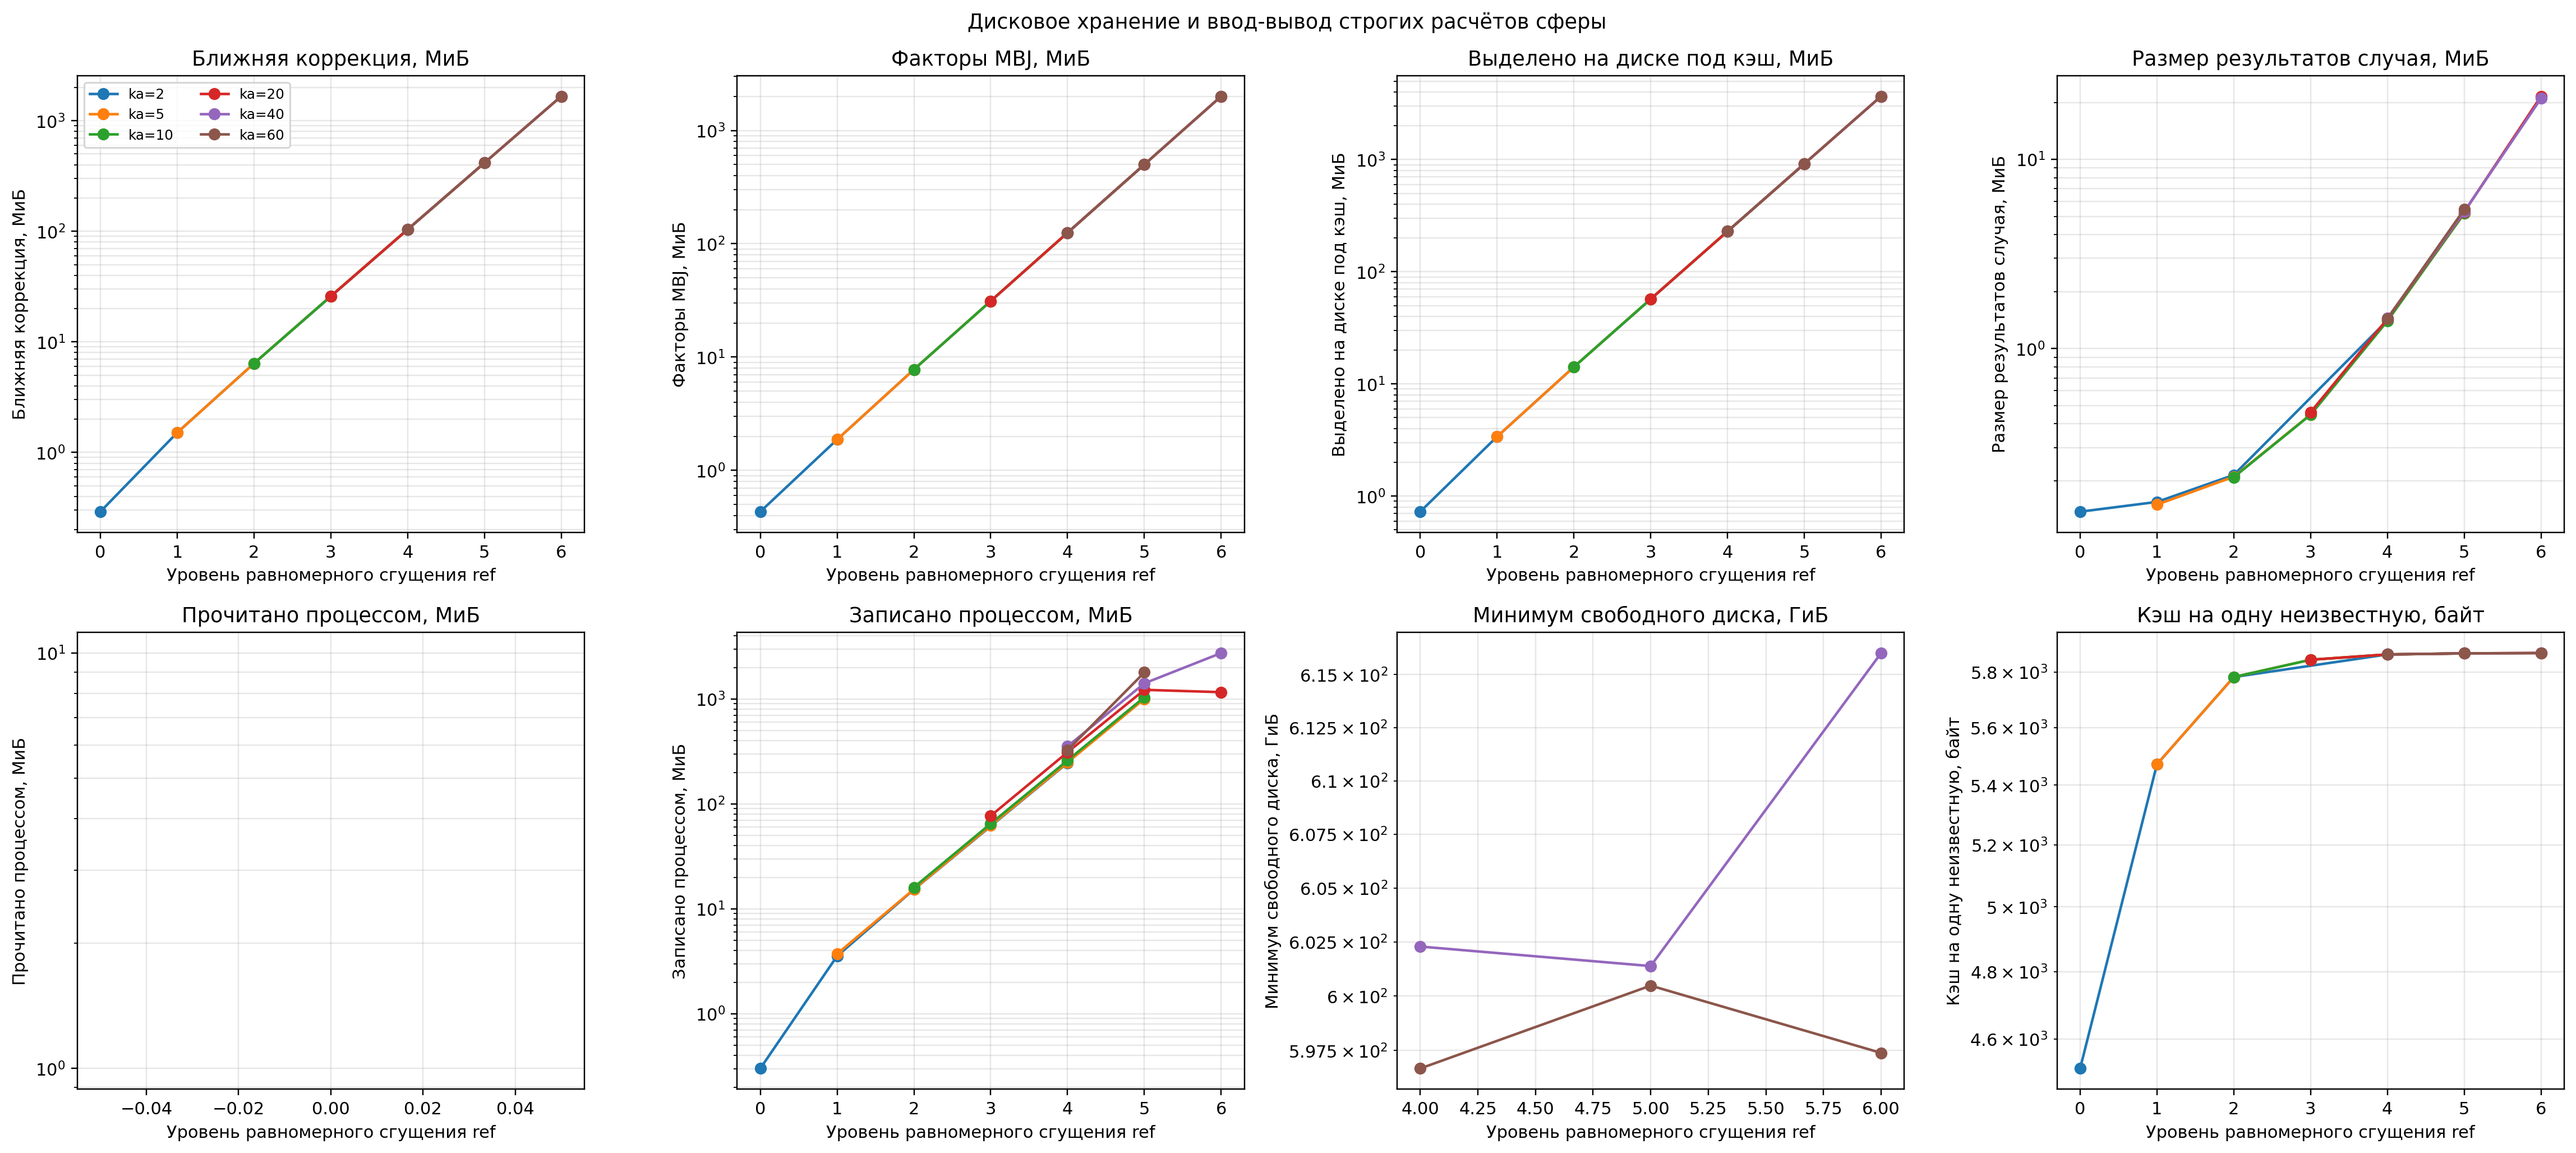
\includegraphics[width=\textwidth]{mesh_ref_ka_storage_resources.png}
  \caption{Дисковые ресурсы: размер кэшей точной ближней коррекции и MBJ,
  размер результатов, а также накопленный ввод-вывод процесса. Логический
  размер файла и число фактически выделенных блоков показаны отдельно.
  Итоговый объём всего исследования в \texttt{summary.json} дедуплицируется по
  устройству и inode, поэтому жёсткие ссылки на прошедший барьер памяти не
  считаются дважды.}
  \label{fig:storage-resources}
\end{figure}

Для завершённых кэшей сферы при фиксированных квадратуре 13, Даффи 6,
$R=5$, листе 64 и MBJ-блоке 50 после выхода из малых сеток наблюдается почти
линейный закон хранения. При \texttt{ref}=5 сумма двух кэшей равна
961~555~580 байт для 163~848 неизвестных, то есть 5868.6 байт на
неизвестную. Барьер памяти \texttt{ref}=6 дал 3~846~887~324 байт для
655~368 неизвестных, или 5869.8 байт на неизвестную. Это измеренный закон
данной структуры данных, а не универсальная константа BEM: радиус, квадратура,
MBJ-блок и базис изменят коэффициент.

\begin{figure}[H]
  \centering
  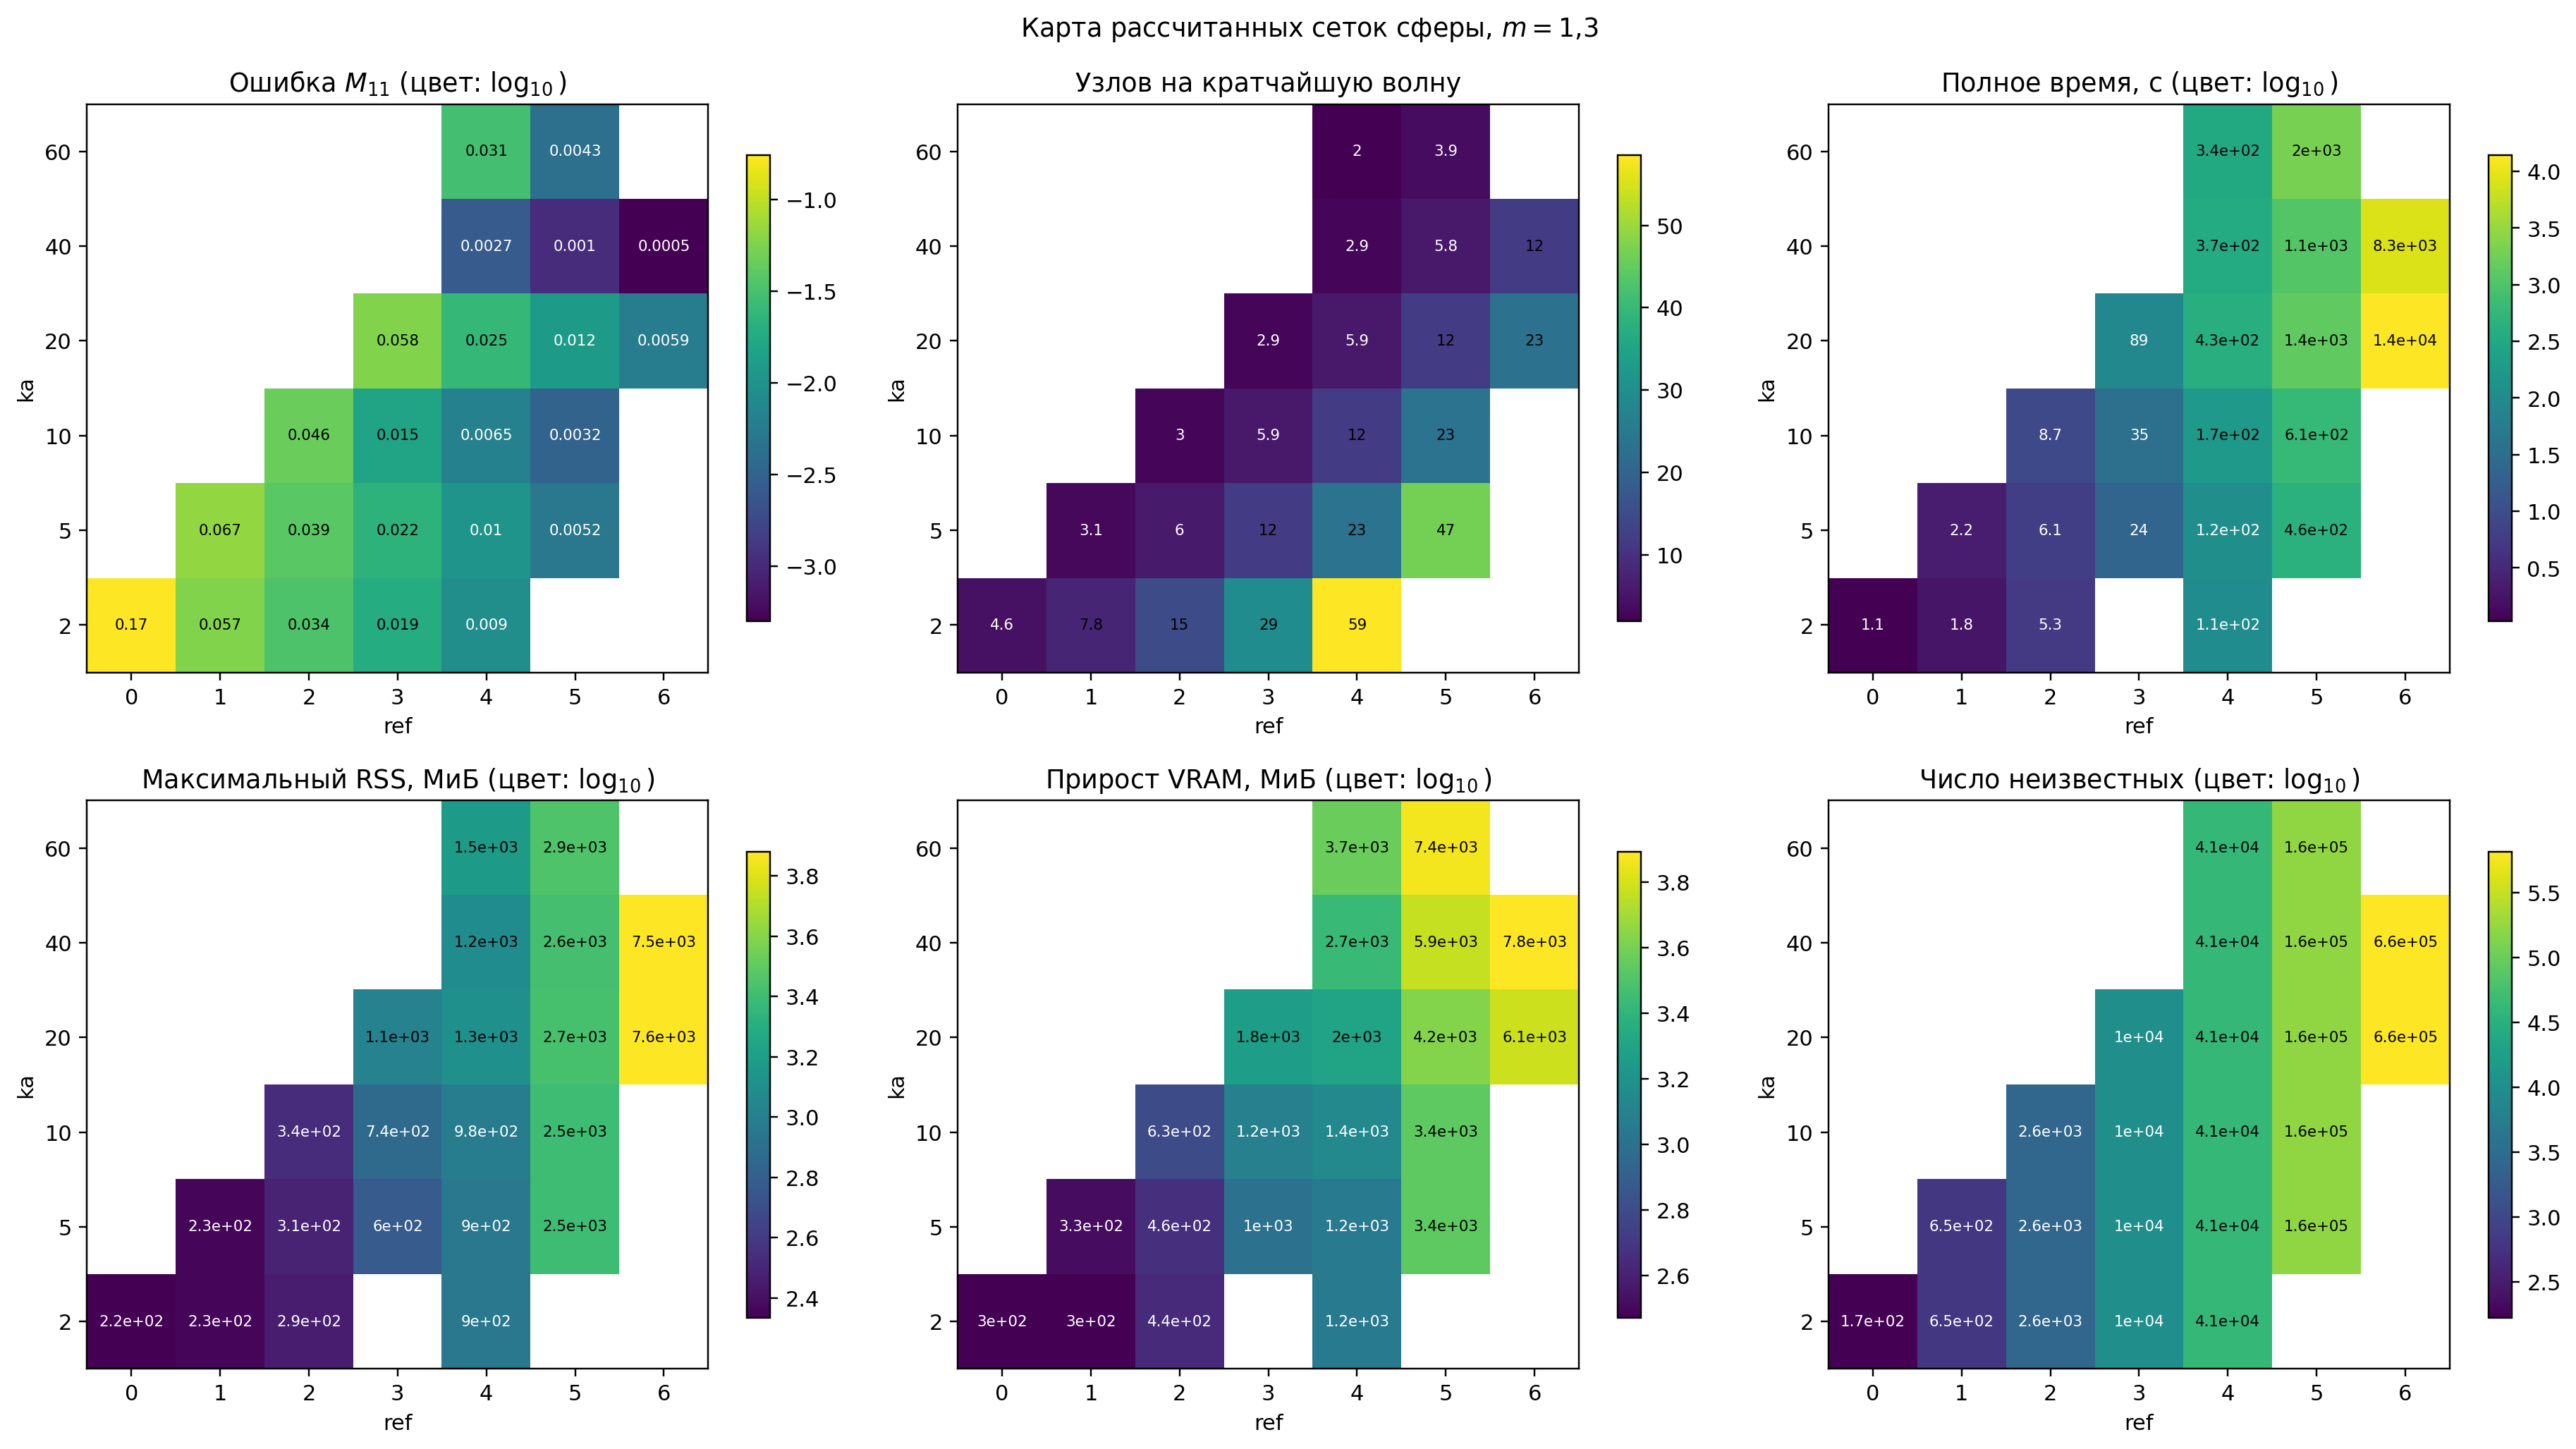
\includegraphics[width=\textwidth]{mesh_ka_ref_heatmaps.png}
  \caption{Карта уже рассчитанных сочетаний $ka$ и \texttt{ref}. Подписи в
  клетках приведены в физических единицах, цвет логарифмический там, где это
  указано.}
  \label{fig:mesh-map}
\end{figure}

\subsection{Влияние показателя преломления}

Контрастная серия показывает, что одно число узлов на кратчайшую внутреннюю
волну не является универсальным критерием. При $ka=10$ минимальные сетки,
прошедшие одновременно пять 1\%-критериев точного решения Ми, равны
\texttt{ref}=5, 4, 5 и 3 для $m=1.1$, 1.5, 2.0 и 2.5 соответственно.
Соответствующие значения $P_{\min}$ равны 27.64, 10.14, 15.20 и 3.05.
Немонотонность не является ошибкой анализа: при слабом рассеянии относительная
ошибка масштаба особенно чувствительна к малому знаменателю, а при других
контрастах положение резонансов меняет чувствительность отдельных метрик.

Для проверки переноса на крупную задачу рассчитана сфера $ka=40$ на
\texttt{ref}=5, то есть при 163~848 неизвестных. При $m=1.5$ ошибки
$M_{11}$, полной нормированной матрицы, направления вперёд и интеграла равны
0.422, 0.226, 0.287 и 0.170\%; обе поляризации достигли истинной невязки
ниже $10^{-3}$ за 205 и 157 итераций. При $m=2.0$ те же ошибки равны 0.110,
0.141, 0.014 и 0.269\%, однако потребовались уже 533 и 561 итерация.
Именно итерационная сходимость, а не пространственная сетка, стала узким
местом высокого контраста. Увеличение рестарта FGMRES со 100 до 200 улучшило
снижение невязки за цикл примерно с 1.96 до 3.28 раза; стоимость
ортогонализации при этом оставалась менее одного процента стоимости действия
оператора.

\begin{figure}[H]
  \centering
  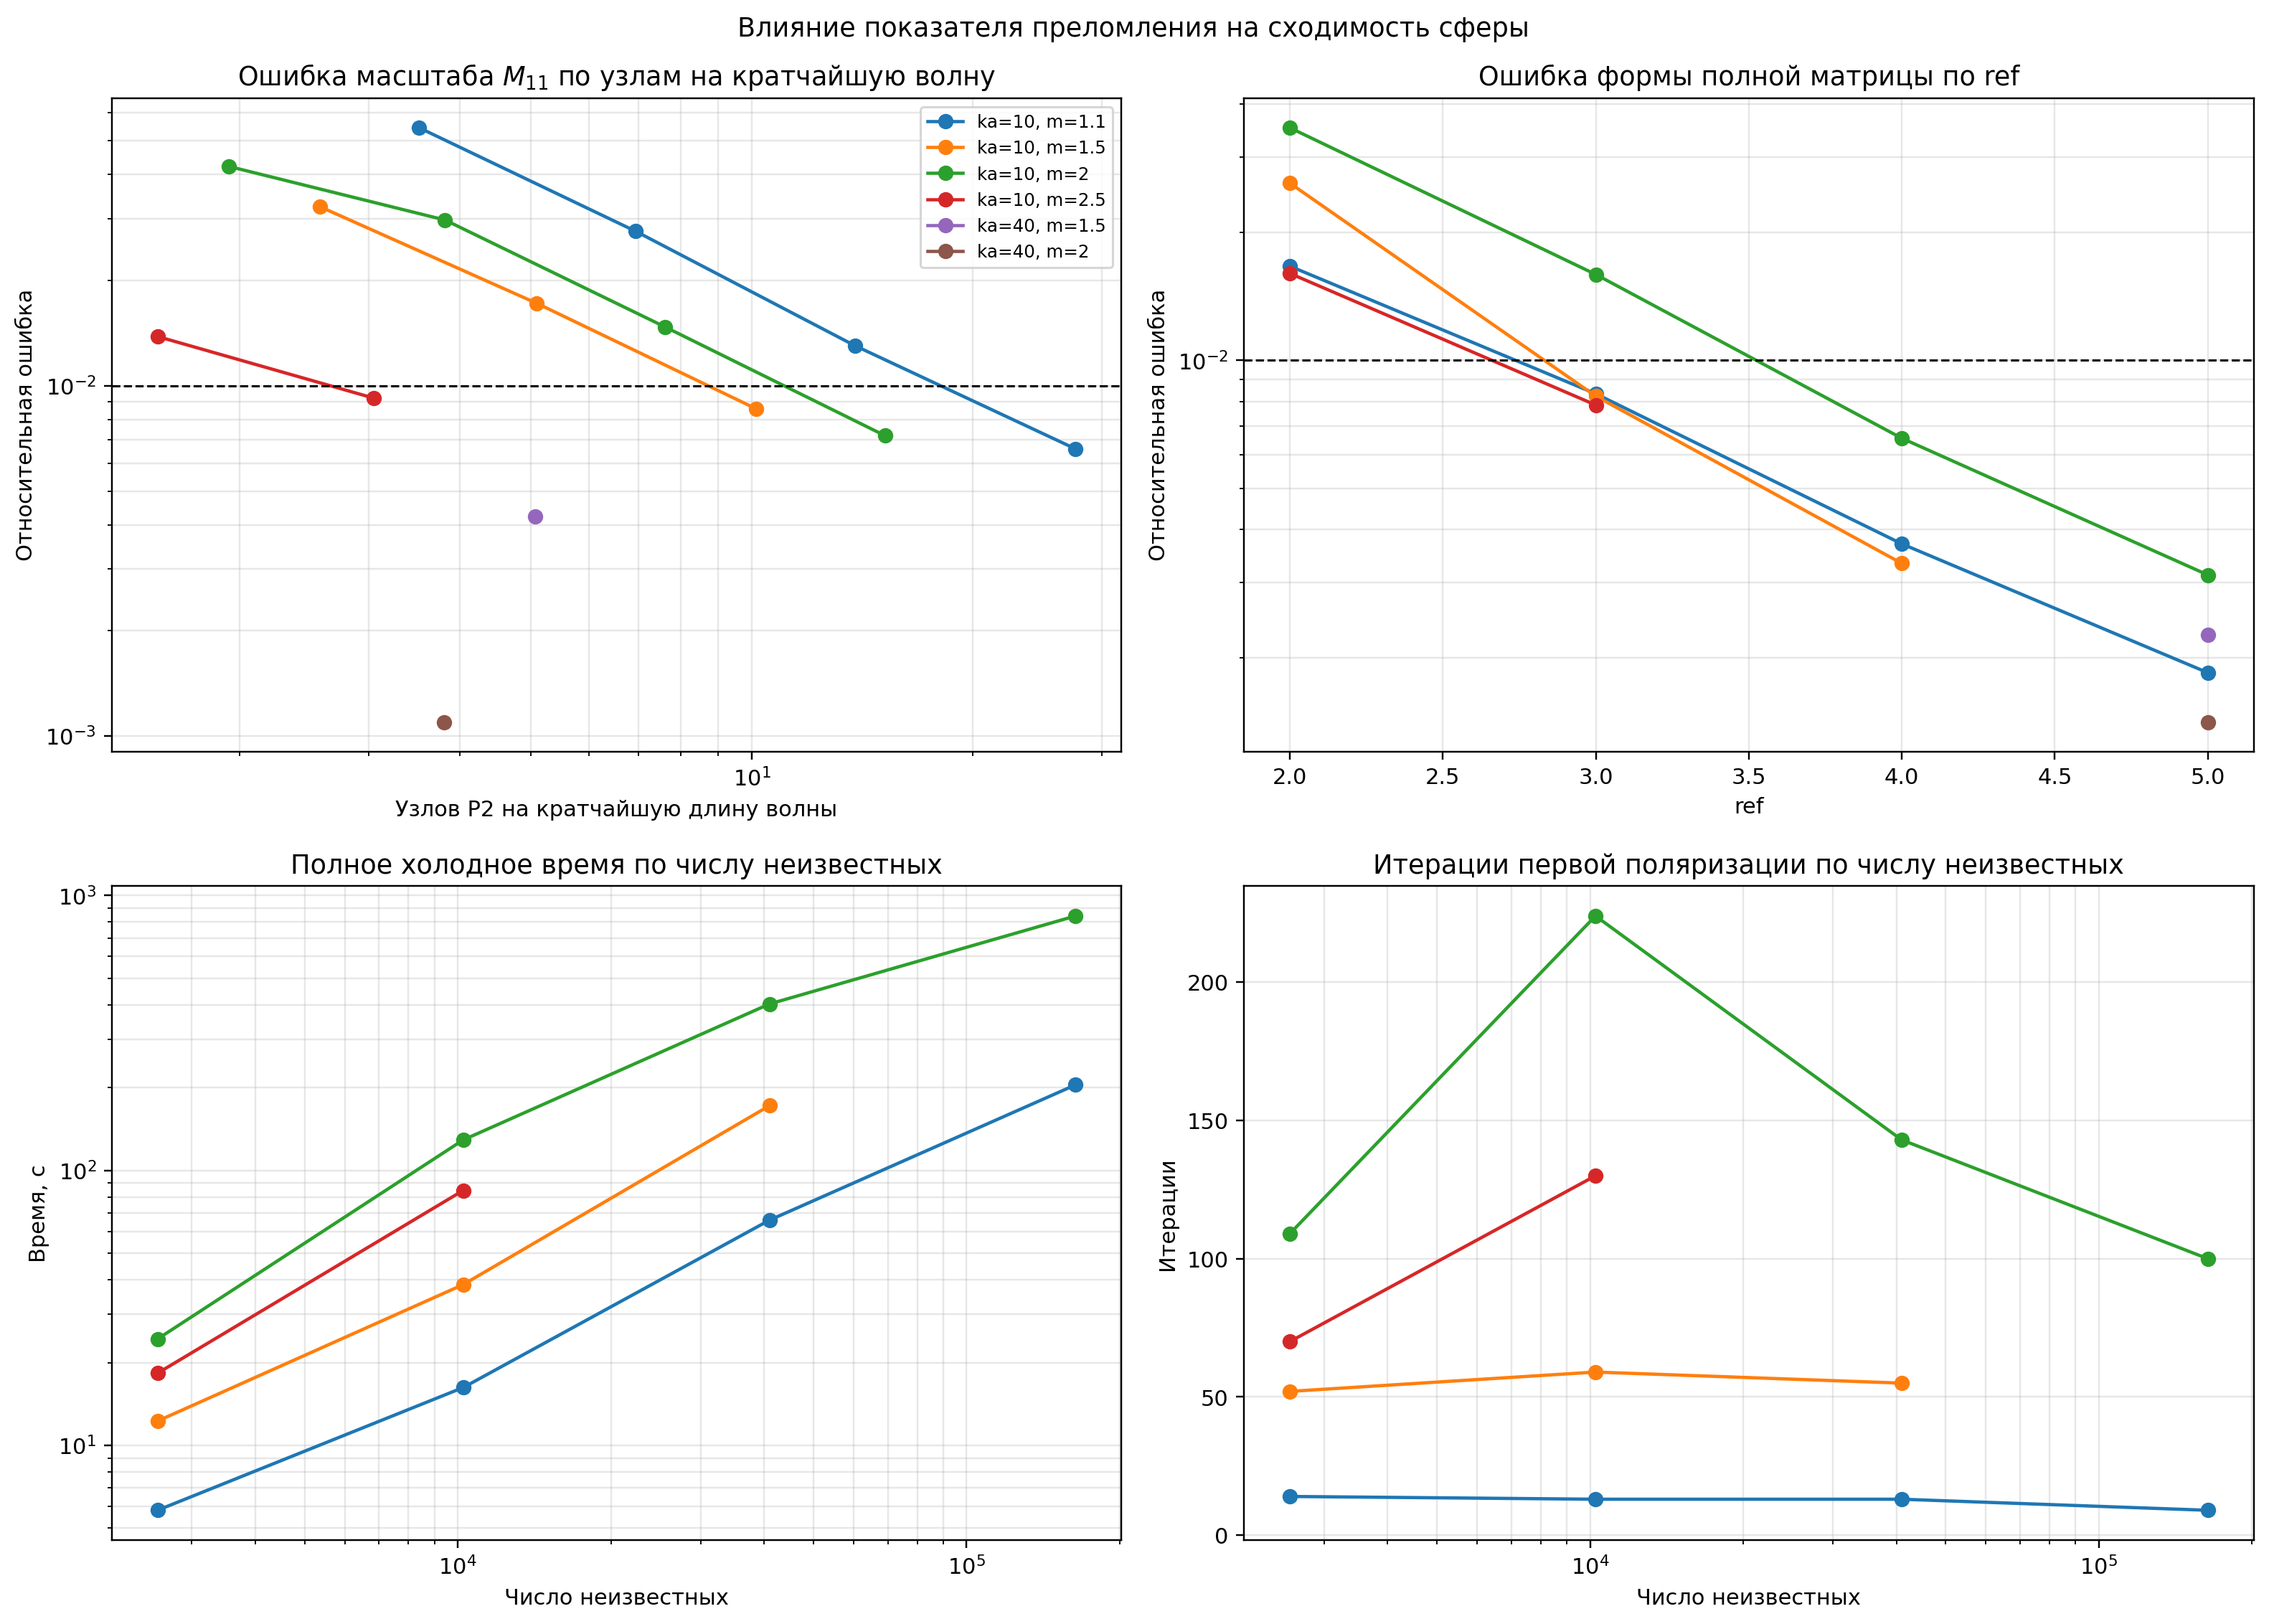
\includegraphics[width=0.94\textwidth]{mesh_sphere_contrast.png}
  \caption{Сходимость сферы при разных показателях преломления. Верхние панели
  показывают ошибку относительно Ми, нижние --- холодное время и число
  итераций первой поляризации. Линия 1\% является применённым
  критерием принятия, а не аппроксимацией данных.}
  \label{fig:mesh-contrast}
\end{figure}

\subsection{Калибровка точности вычислений}

На сфере $ka=2$, $m=1.3$, \texttt{ref}=1 смешанный и FP64-пути дали
относительное отличие полной ненормированной матрицы порядка
$3.35\cdot10^{-7}$ и отличие $M_{11}(0)$ порядка $2.57\cdot10^{-7}$. Это
показывает, что смешанная точность перспективна для производительного режима,
но сеточная статья использует более строгий FP64-контроль, чтобы не смешивать
ошибки.

Холодный FP64-процесс занял около 1.28~с, тёплый --- 0.47~с; для смешанного
пути соответственно около 0.79 и 0.28~с. Эти числа нельзя экстраполировать на
крупные сетки, но они подтверждают работоспособность раздельного учёта кэша.

\subsection{Первые результаты по радиусу FMM}

Для сферы $ka=5$, $m=1.3$, \texttt{ref}=3, \texttt{digits}=7, листа 64 и
невязки $10^{-4}$ получено:
\begin{table}[H]
\centering
\caption{Холодная стоимость радиуса ближней зоны. Ошибка измерена относительно
$R=5$ на той же сетке и не является сеточной ошибкой относительно Ми.}
\resizebox{\textwidth}{!}{%
\begin{tabular}{rrrr}
\toprule
$R$ & полное время, с & прирост VRAM, МиБ & $E_{\mathrm{full}}$ относительно $R=5$\\
\midrule
1 & 10.84 & 828  & $1.77\cdot10^{-4}$\\
3 & 14.34 & 898  & $3.05\cdot10^{-8}$\\
5 & 20.53 & 1004 & 0\\
\bottomrule
\end{tabular}
}
\end{table}
Радиус 1 в этом низкоконтрастном случае меняет полную нормированную матрицу
лишь на 0.0177\% и быстрее радиуса 3 примерно в 1.32 раза. Однако при строгой
невязке $2\cdot10^{-6}$ он достиг плато около $3.4\cdot10^{-5}$. Кроме того,
предыдущий независимый контроль на призме $ka=20$, $m=3$ показал, что малый
радиус может давать ошибку оператора порядка $10^{-3}$--$10^{-2}$. Поэтому
$R=1$ нельзя объявить универсальным; текущая рекомендация $R=3$ остаётся до
завершения масштабной и контрастной серии.

На сфере $ka=20$, $m=1.3$, \texttt{ref}=5 та же серия дала более жёсткое
разделение режимов. При $R=1$ полный холодный процесс занял 234.25~с, а ошибка
$M_{11}$ относительно Ми составила 1.641\%. При $R=3$ время выросло до
493.81~с, но ошибка $M_{11}$ уменьшилась до 1.210\%; при $R=5$ время достигло
969.48~с, тогда как ошибка осталась 1.210\%. Отличие полной нормированной
матрицы между $R=3$ и $R=5$ равно $1.85\cdot10^{-7}$, поэтому для данной
сетки $R=3$ уже достиг радиусного предела. Оставшиеся 1.21\% нельзя исправить
дальнейшим ростом $R$: это преимущественно дискретизационная ошибка
\texttt{ref}=5. Цена одной итерации при переходе $R=1\to3\to5$ выросла
примерно с 1.22 до 4.4 и 10.0~с, тогда как число итераций изменилось лишь с
$45+44$ до $41+41$. Следовательно, большой радиус следует выбирать по
точности, а не как средство ускорения решателя.

\paragraph{Ложная самосходимость при большом электрическом размере.}
Для сферы $ka=40$, $m=1.3$, \texttt{digits}=7 и $R=1$ получен принципиально
важный отрицательный результат. Сетки \texttt{ref}=5 и \texttt{ref}=6
различаются всего на 0.0657\% по ненормированному $M_{11}$ и на 0.0993\% по
полной нормированной матрице Мюллера. Если проверять только две соседние сетки,
это выглядит как убедительная сходимость. Однако аналитическое решение Ми даёт
ошибку $M_{11}$ соответственно 15.12\% и 15.15\%, а ошибку полной
нормированной матрицы 3.43\% и 3.48\%. Ошибка в направлении вперёд остаётся
около 13.1\%. Следовательно, измельчение поверхностной сетки не исправляет
систематическую ошибку приближённого FMM-оператора; две сетки могут сходиться к
одному неверному результату. Близость более грубой \texttt{ref}=4 к решению Ми
в этом случае является случайной компенсацией ошибок и не может использоваться
для выбора сетки. Поэтому для сферы одновременно обязательны проверка по Ми и
радиусная серия, а для несферических частиц требуется независимый эталон либо
совместное уточнение сетки и параметров FMM.

Повтор того же случая \texttt{ref}=6 с $R=3$ устранил систематическую ошибку:
$M_{11}$ отличается от Ми на 0.0501\%, значение в направлении вперёд --- на
0.0374\%, интеграл $M_{11}$ --- на 0.0366\%, полная нормированная матрица ---
на 0.0734\%, максимальное абсолютное отличие её нормированных элементов ---
на 0.0298\%. Обе поляризации достигли истинной невязки $10^{-4}$ за 79 и 81
итерацию вместо $135+135$ при $R=1$. Однако действие оператора стало дороже:
решение с готовым кэшем заняло 8309.9~с, а восстановленная оценка одного
холодного процесса с учётом сборки оператора --- около 8771~с против 3731~с
для $R=1$. Следовательно, $R=3$ увеличил точность более чем на два порядка и
сократил число итераций в 1.69 раза, но полное холодное время выросло примерно
в 2.35 раза.

Промежуточный радиус $R=2$ не сохранил точность: ошибка $M_{11}$ равна
15.31\%, ошибка вперёд --- 14.05\%, ошибка интеграла --- 7.59\%, а полная
нормированная ошибка --- 2.57\%. Результат отличается от $R=3$ на 15.31\% по
$M_{11}$. Обе поляризации потребовали $130+130$ итераций, холодное время
составило 7780~с. Таким образом, $R=2$ экономит лишь около 11\% холодного
времени относительно $R=3$, но увеличивает ошибку $M_{11}$ более чем в 300
раз. Для данной точки наблюдается резкий порог между $R=2$ и $R=3$;
минимальный проверенный корректный радиус равен трём ячейкам.

\begin{figure}[H]
  \centering
  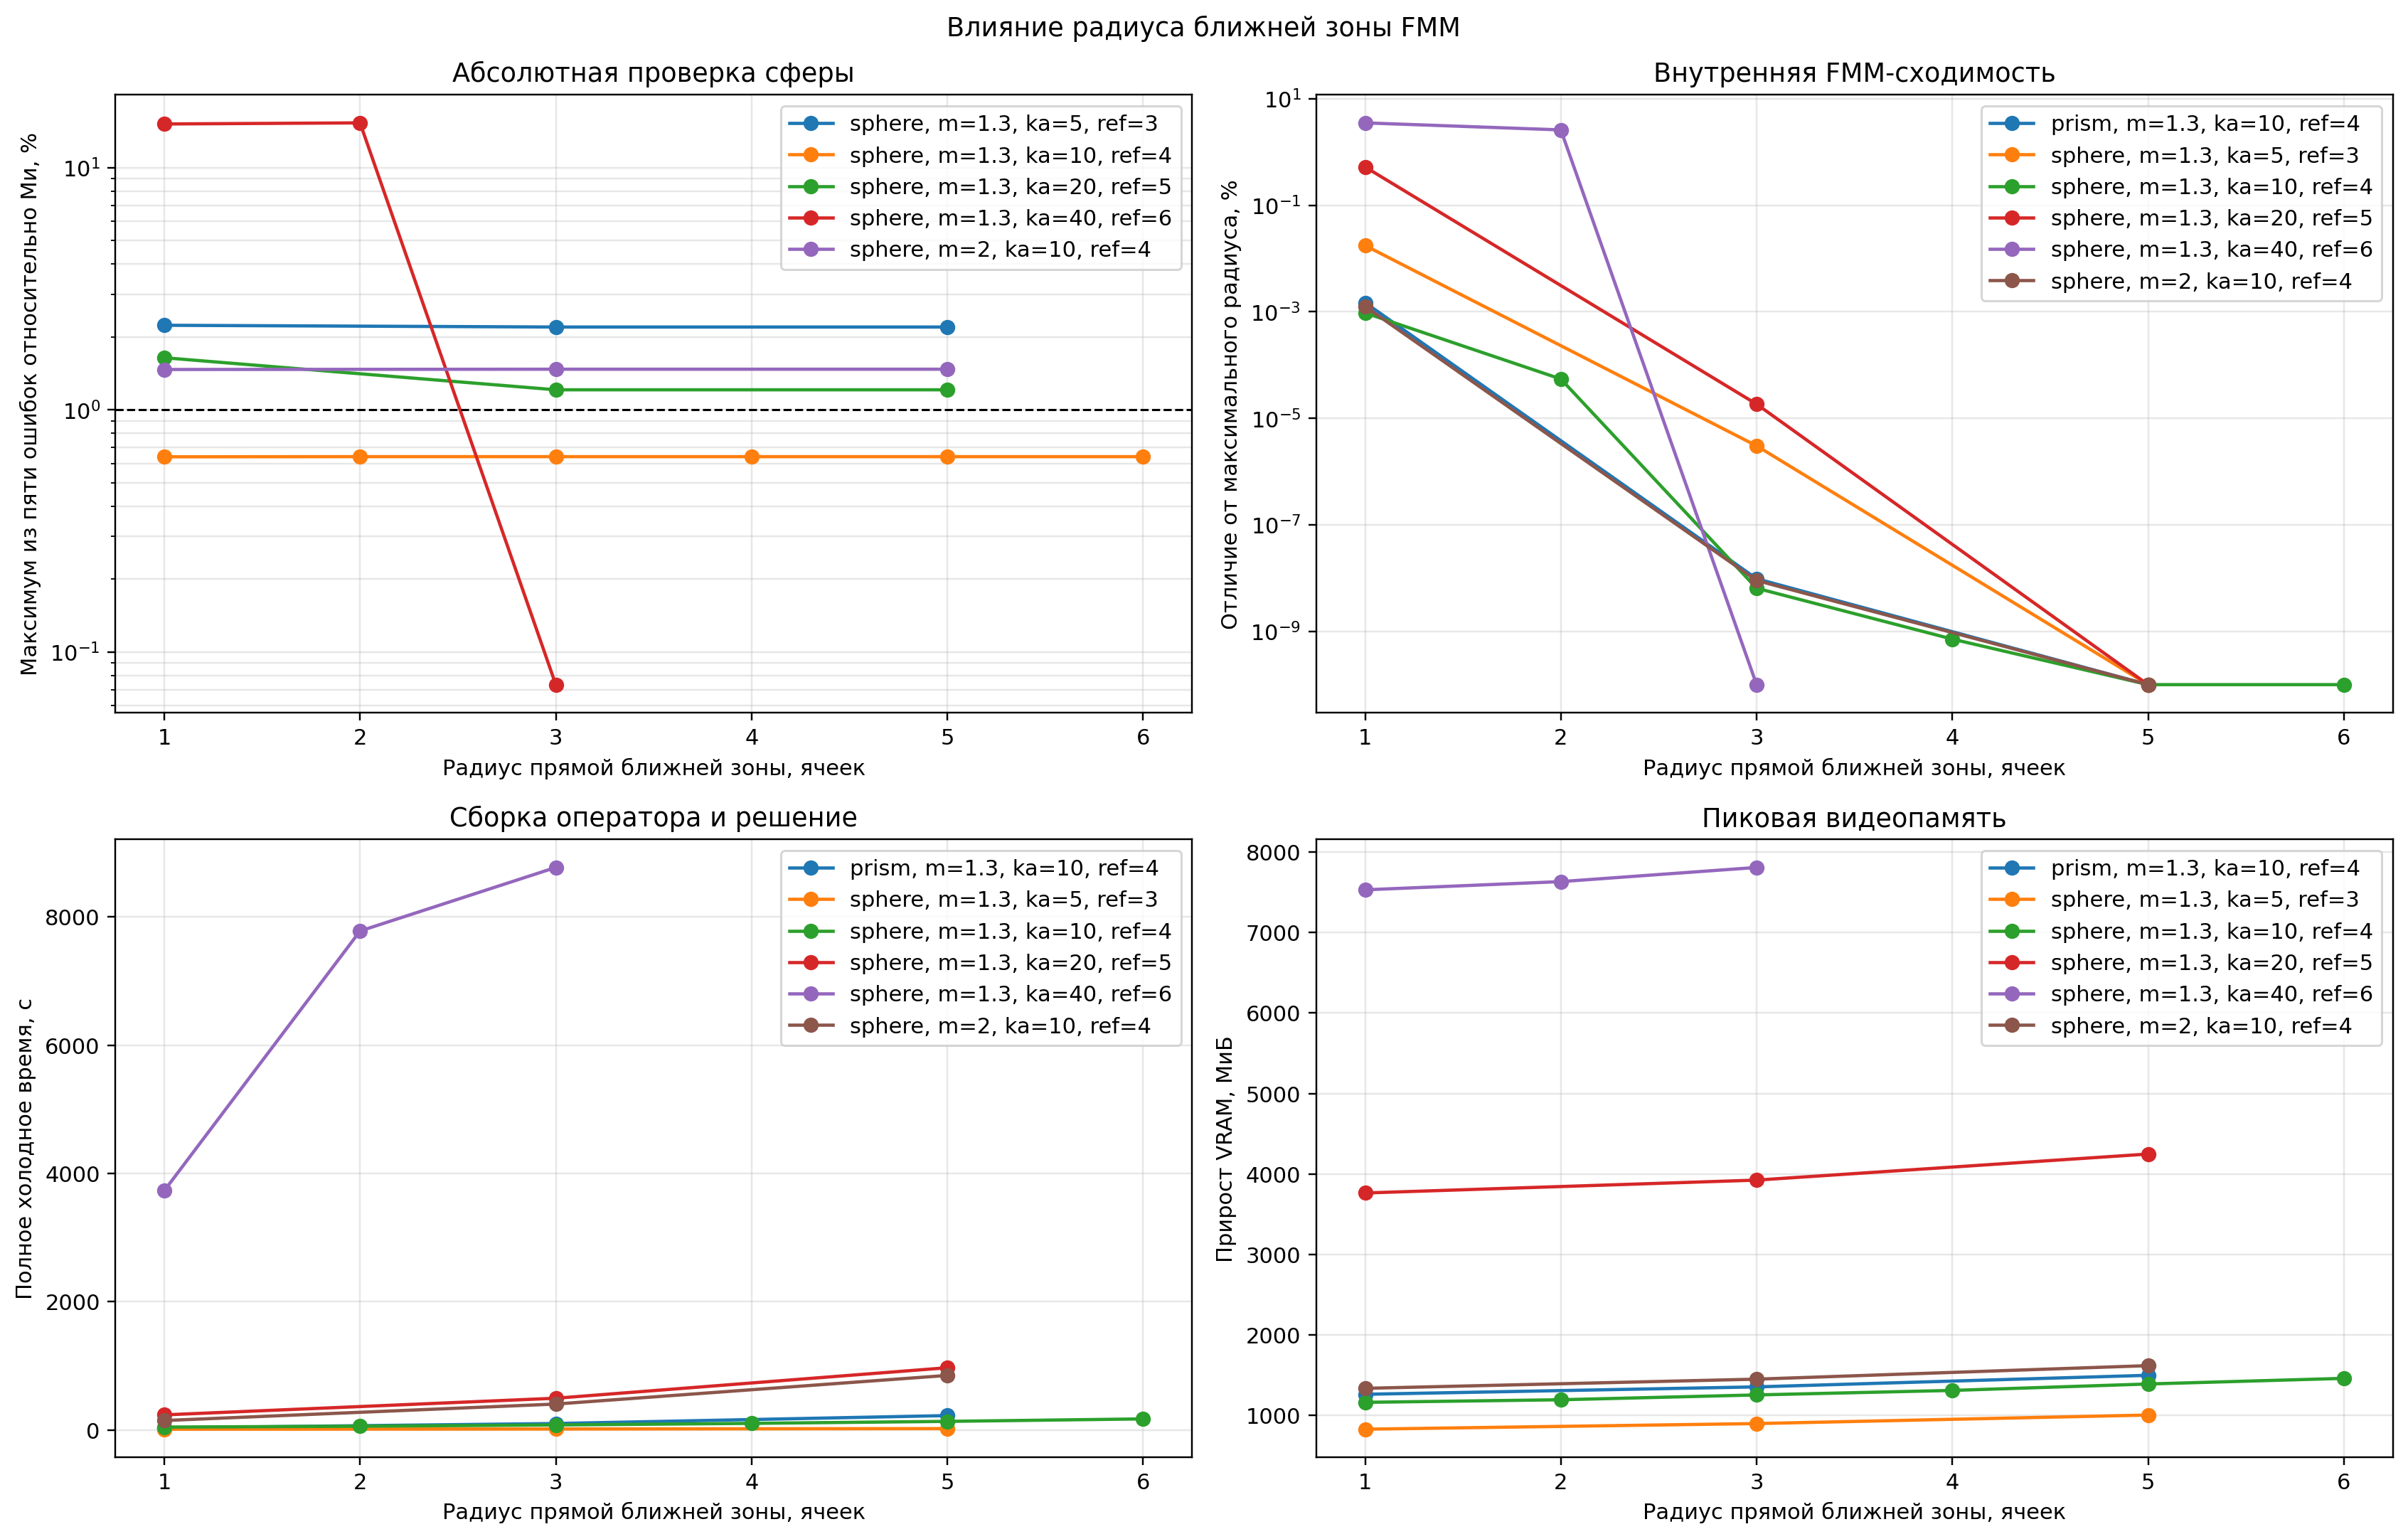
\includegraphics[width=\textwidth]{fmm_near_radius_tradeoff.png}
  \caption{Компромисс между отличием физического результата, временем и VRAM
  при изменении радиуса ближней зоны FMM.}
  \label{fig:fmm-radius}
\end{figure}

\subsection{Промежуточная стоимость крупных точек}

Для $ka=5$, \texttt{ref}=5 система имела 163848 комплексных неизвестных и
266240 квадратурных источников. Полный холодный процесс занял 456.2~с,
максимальный RSS --- 2503~МиБ, прирост VRAM --- 3448~МиБ. Построение FMM заняло
85.1~с, MBJ --- 38.0~с, каждое из двух решений --- около 166~с при 16
итерациях. Эти внутренние времена объясняют, почему полная стоимость не равна
только числу итераций, и показывают, какие части можно амортизировать по многим
ориентациям.

Для $ka=20$, \texttt{ref}=4 получено 40968 неизвестных, 65 и 64 итерации,
426.9~с холодного времени, 1291~МиБ RSS и около 2006~МиБ прироста VRAM. При
том же числе неизвестных случай $ka=10$, \texttt{ref}=4 занял 172.8~с и 24
итерации. Следовательно, $N$ само по себе не задаёт время: электрический размер
увеличил порядок/стоимость действия и ухудшил итерационную сходимость.

Следующая точка $ka=20$, \texttt{ref}=5 содержит 163848 неизвестных и 266240
квадратурных источников. Обе поляризации потребовали по 60 итераций, истинные
невязки составили $1.61\cdot10^{-6}$ и $1.69\cdot10^{-6}$. Холодное время
равно 1353.3~с, RSS --- 2689~МиБ, прирост VRAM --- 4248~МиБ. Ошибка
$E_{11}^{\mathrm{raw}}=1.207\%$ ещё немного превышает порог 1\%, хотя ошибка
формы полной нормированной матрицы уже равна 0.446\%. Поэтому точка
\texttt{ref}=6 необходима не ради уменьшения невязки, а ради сеточной
сходимости физического масштаба.

Расчёт $ka=20$, \texttt{ref}=6 содержит 655368 комплексных неизвестных,
81920 треугольников и 1064960 квадратурных источников; $P_{\min}=23.38$.
Обе поляризации сошлись за 57 итераций с истинными невязками
$1.809\cdot10^{-6}$ и $1.921\cdot10^{-6}$. При уже подготовленных кэшах полное
время процесса составило 13920~с, из которых 13910.9~с заняли два решения;
максимальный RSS равен 7589~МиБ, прирост VRAM --- 6112~МиБ, средняя загрузка
GPU --- 99.67\%. Получены
$E_{11}^{\mathrm{raw}}=0.588\%$, ошибка вперёд 0.552\%, ошибка интеграла
0.349\% и ошибка полной нормированной матрицы 0.214\%. Таким образом,
\texttt{ref}=6 проходит все принятые 1\%-критерии точного эталона Ми, тогда как
\texttt{ref}=5 не проходил по ненормированному $M_{11}$. Это подтверждает
минимальный уровень среди рассчитанных сеток; значение не переносится на
другие формы и показатели преломления.

\subsection{Масштабирование расчёта призмы}

Для шестигранной призмы с H(div)-BDM1 выполнено по три запуска на каждом из
пяти уровней. Первый запуск включает построение кэшей, два следующих повторно
используют их. Результаты сведены в табл.~\ref{tab:prism-resource-scaling}.
Все времена являются полным стеночным временем процесса с двумя независимыми
поляризациями и истинной невязкой $10^{-5}$.

\begin{table}[H]
\centering
\caption{Измеренное масштабирование производственного смешанного пути. Тёплое
время --- среднее двух повторов с готовыми кэшами.}
\label{tab:prism-resource-scaling}
\resizebox{0.96\textwidth}{!}{%
\begin{tabular}{rrrrrrr}
\toprule
$ka$ & \texttt{ref} & неизвестных & холодное время, с & тёплое время, с & RAM, МиБ & VRAM, МиБ\\
\midrule
5  & 2 & 3~168   & 1.06   & 0.63   & 282  & 269\\
10 & 3 & 12~672  & 2.44   & 1.17   & 397  & 816\\
20 & 4 & 50~688  & 9.14   & 4.59   & 904  & 2~318\\
30 & 5 & 202~752 & 39.46  & 22.10  & 2~673 & 6~512\\
40 & 6 & 806~400 & 227.25 & 159.10 & 9~058 & 19~670\\
\bottomrule
\end{tabular}}
\end{table}

При каждом повышении \texttt{ref} число неизвестных возрастает примерно
вчетверо, но тёплое время растёт не с постоянным коэффициентом: от 1.86 до
7.20 между соседними строками. Кэш ускоряет полный процесс в 1.43--2.09 раза,
причём его относительная польза уменьшается по мере перехода стоимости к
итерационным действиям оператора. В исходной реализации точка $ka=40$,
\texttt{ref}=6 занимала 19.67~ГиБ VRAM на RTX~3090~Ti с 24~ГиБ. Линейная
экстраполяция этого прежнего четырёхполевого хранения на \texttt{ref}=7 давала
около 78.7~ГиБ. Эта величина описывает ограничение старой схемы массивов, а не
неустранимый предел метода.

После основной серии FMM переработан: фиксированная ориентация резервирует
только три векторные компоненты, необходимые для одного действия оператора,
а четырёхполевой буфер сохраняется только для парного ориентационного режима.
Контрольная призма $ka=40$, \texttt{ref}=7 содержит 3~225~600 комплексных
неизвестных и 537~600 треугольников. Измеренный прирост VRAM равен
16~290~МиБ (15.91~ГиБ), а полный пик занятости карты --- 16~587~МиБ
(16.20~ГиБ). Реальное действие FMM занимает около 29.5~с и выполняется при
полной загрузке GPU. MBJ(12) хранит 2.39~ГиБ факторов в оперативной памяти и загружается из
кэша менее чем за секунду. Возобновляемое решение достигло 123 накопленных
итераций и непосредственно проверенной FMM-невязки
$9.842\cdot10^{-6}$. Следовательно, \texttt{ref}=7 не только строится, но и
строго решается на этой аппаратуре. Из-за нескольких преднамеренных остановок
суммарное стеночное время этого контроля нельзя использовать как чистый
производительный эталон. Перенос результата на $ka=60$ пока не делается:
зависимость порядка разложения FMM от электрического размера требует
отдельного измерения.

\begin{figure}[H]
  \centering
  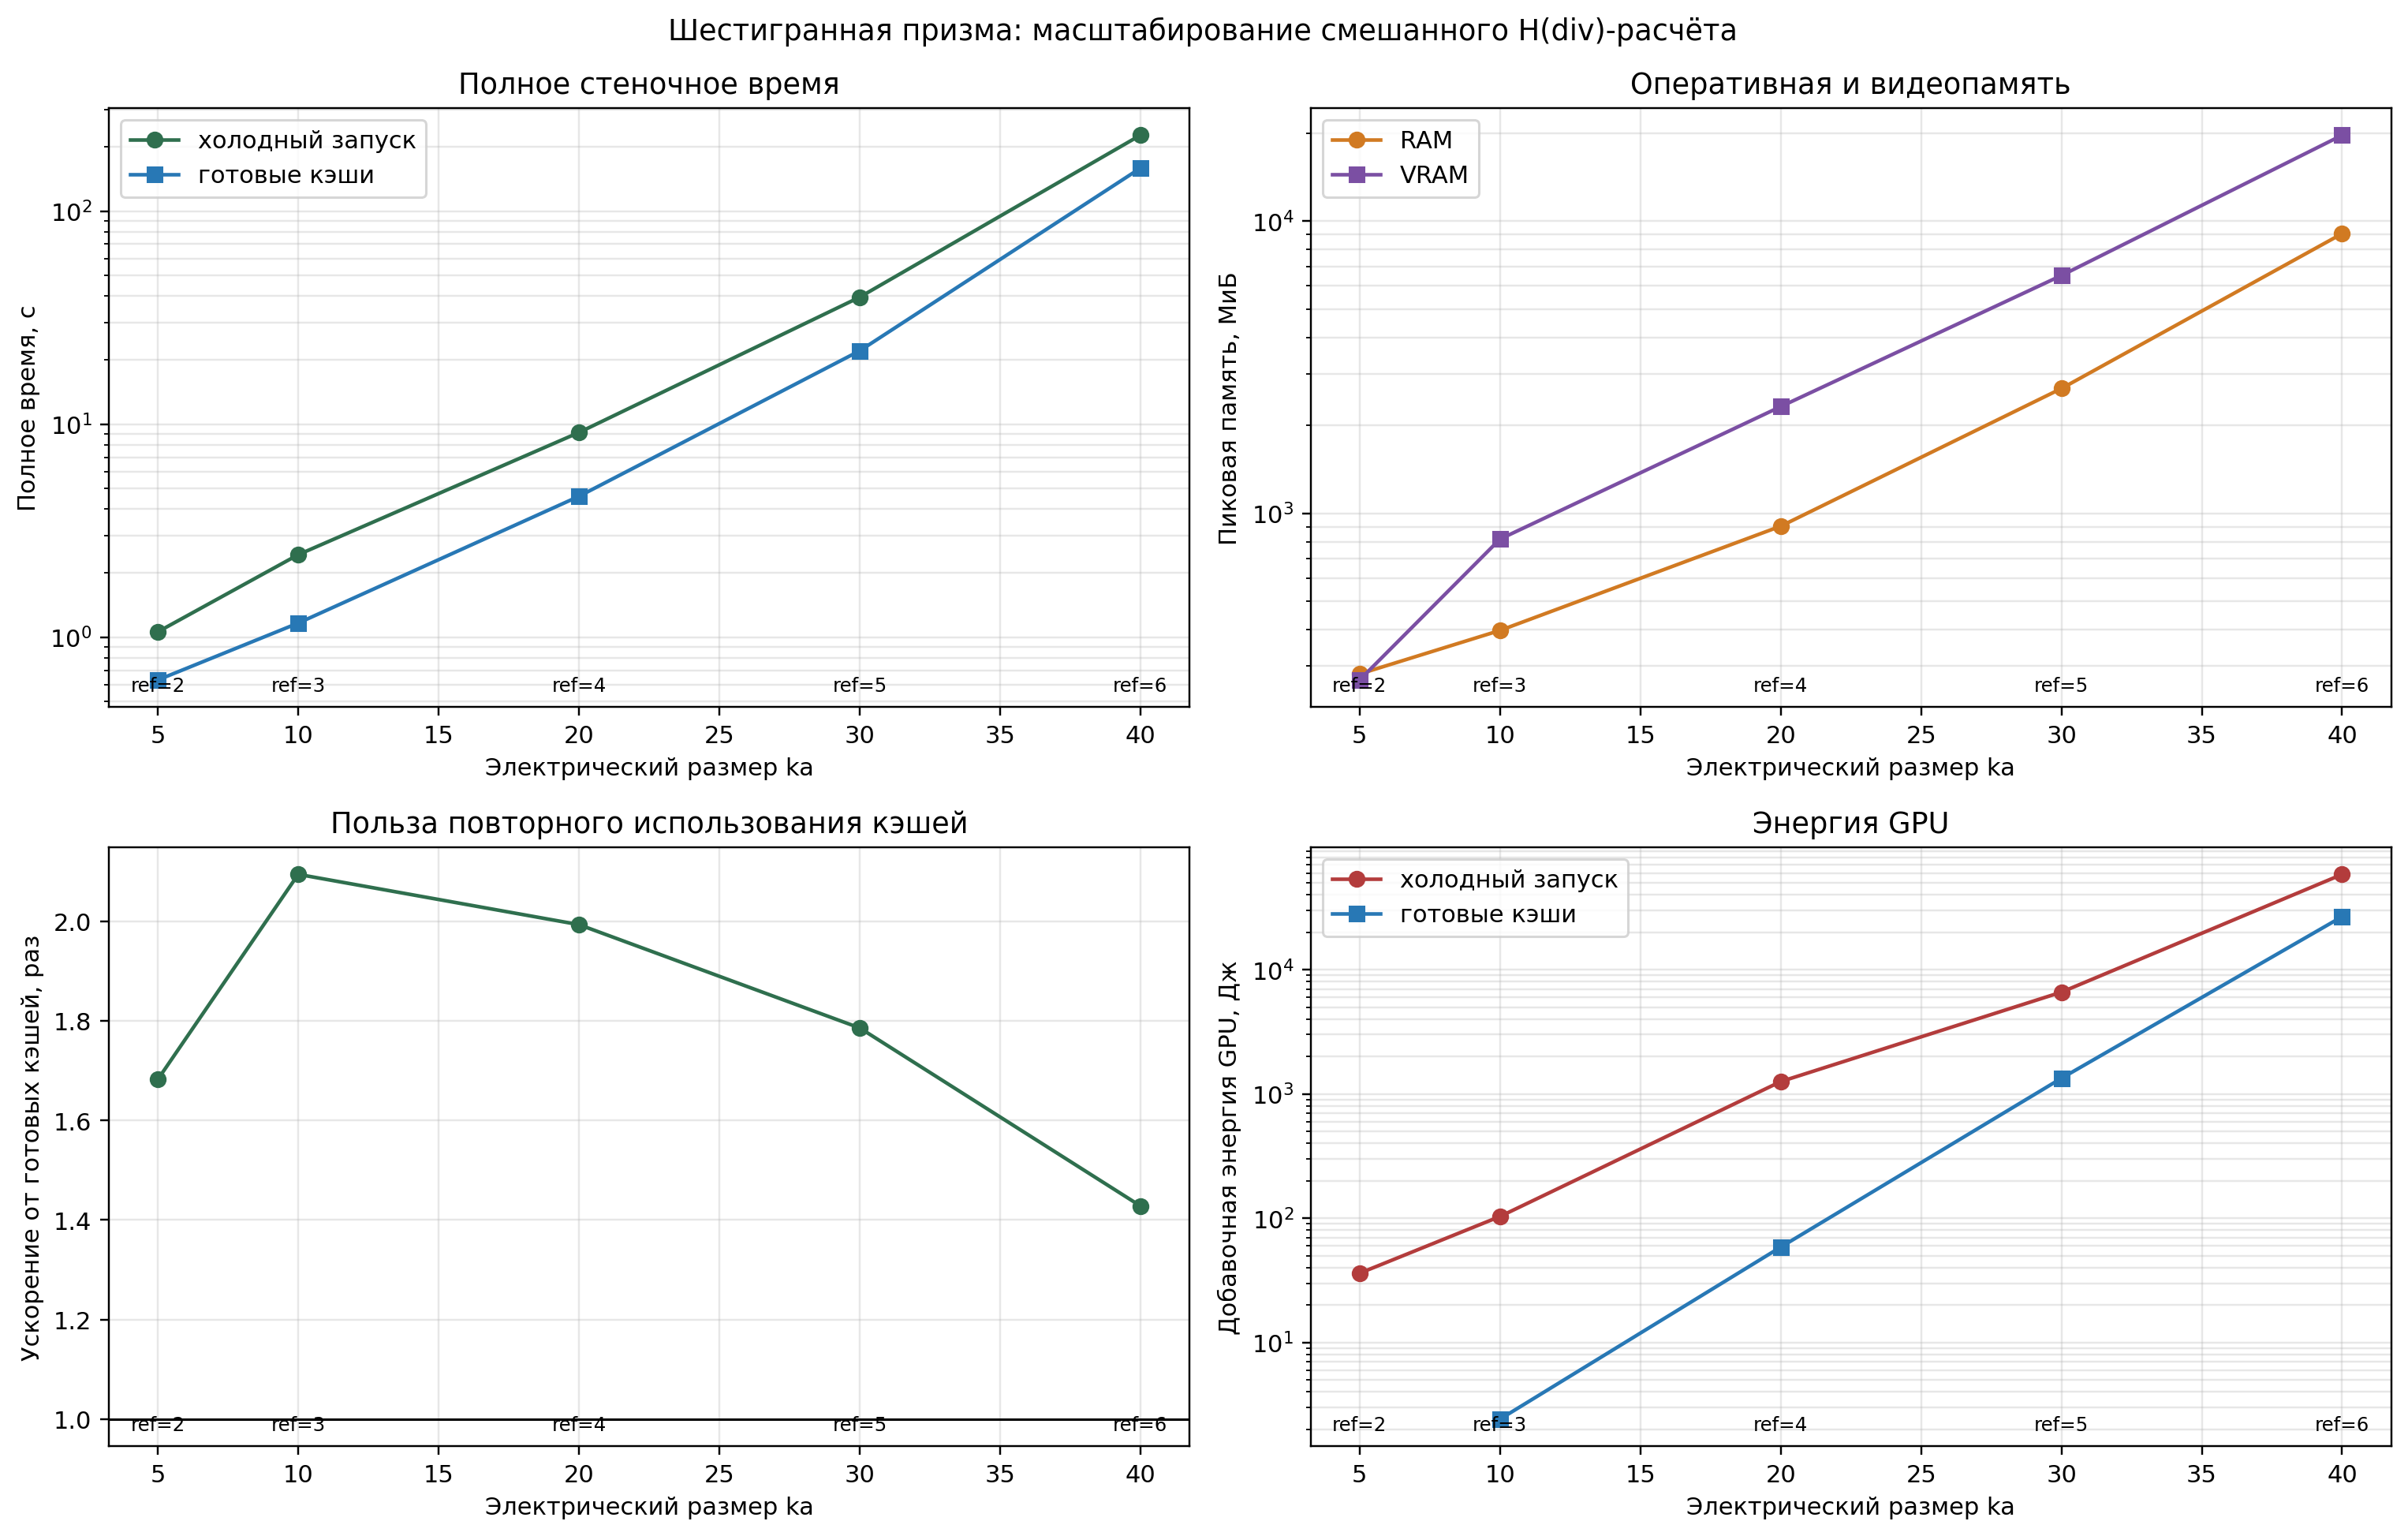
\includegraphics[width=0.98\textwidth]{production_resource_scaling.png}
  \caption{Отдельная ресурсная серия H(div)-призмы. Холодное время включает
  построение кэшей, тёплое является средним двух повторов. Энергия коротких
  запусков диагностическая из-за конечного интервала опроса. Исходная таблица
  находится в \texttt{production\_\allowbreak resource\_\allowbreak scaling.csv}.}
  \label{fig:production-resource-scaling}
\end{figure}

Исторический прогноз следующего уровня хранится в отдельном машиночитаемом
JSON-файле. Он явно помечен как линейная экстраполяция прежнего хранения, а не
измерение текущей реализации:
$N=3\,225\,600$, требуемая VRAM 78~680~МиБ, отношение к фактической ёмкости
карты 3.20.

\section{Правила выбора параметров}

\subsection{Число базисных функций и \texttt{ref}}

Для нового случая рекомендуется следующий воспроизводимый алгоритм:
\begin{enumerate}
  \item Выбрать физическую метрику и допуск, например 1\% одновременно для
        \eqref{eq:m11-error}, ошибки вперёд, интеграла и \eqref{eq:full-error}.
  \item По \eqref{eq:ref-start} получить только стартовый \texttt{ref}; для
        гладкой сферы пока разумно использовать консервативное $P_*$ и отдельный
        минимум геометрического сгущения.
  \item Выполнить расчёты на $r$ и $r+1$ с одинаковыми строгими параметрами
        оператора. Если изменение больше допуска, продолжить на $r+2$.
  \item Для острой частицы использовать H(div)-BDM1 и не переносить порог P2
        со сферы. Проверить не менее трёх уровней, поскольку два значения не
        позволяют установить уменьшение ошибки.
  \item Для сферы считать допустимым тот $r$, на котором все метрики точного
        решения Ми проходят порог; сравнение с $r+1$ остаётся дополнительной
        проверкой порядка. Для формы без точного эталона требовать также
        сравнение с $r+1$ и не менее трёх уровней сетки.
\end{enumerate}

Текущая завершённая серия показывает, что автоматическое правило нельзя
строить только по среднему $P_{\min}$. Для расширения области применимости
нужна верхняя огибающая подтверждённых точек, в которую явно войдут $ka$,
контраст $|m^2-1|$, тип геометрии и базиса.

\subsection{Радиус, \texttt{digits} и лист FMM}

Порядок выбора должен быть следующим:
\begin{enumerate}
  \item На фиксированной репрезентативной сетке выбрать строгий эталон с
        большим $R$ и $d$.
  \item При фиксированном листе построить двумерную границу по $(R,d)$, а не
        оптимизировать параметры изолированно.
  \item Отбросить точки, где истинная невязка имеет плато выше рабочего
        допуска, даже если одна физическая кривая случайно близка к эталону.
  \item Среди прошедших точек выбрать минимум полного времени при ограничении
        VRAM. Повторить на малом, среднем и максимальном $ka$, а также на
        высоком контрасте.
  \item После фиксации $(R,d)$ перебрать лист. Записывать фактические глубину,
        лист, $p$ и $L$, иначе результат не переносим.
\end{enumerate}
Текущие данные поддерживают $R=3$ как консервативный рабочий кандидат, но это
ещё не окончательная универсальная рекомендация.

\subsection{Квадратура}

Для гладкой сферы порядок увеличивается до тех пор, пока изменение результата
не станет как минимум в 5--10 раз меньше сеточной ошибки. Для острых рёбер
отдельно повышается Даффи-порядок. Если повышение обычной квадратуры почти не
меняет результат, а Даффи меняет, ошибка локализована в соседних/сингулярных
парах. Если меняются оба, сначала фиксируется более строгая сингулярная часть,
затем повторяется обычная серия.

\subsection{Допуск, число итераций и рестарт}

Рабочий допуск выбирается по фактическому плато истинной невязки и должен быть
существенно ниже целевой физической ошибки. \texttt{max-iters} не является
параметром точности: это аварийный предел. Достигший предела запуск считается
несошедшимся и сохраняется. Размер рестарта выбирается по двум кривым:
итерации/время и пик памяти. При наличии VRAM большой рестарт уменьшает риск
стагнации; при недостатке памяти он может быть уменьшен, но физический результат
принимается только после истинной проверки \eqref{eq:true-residual}.

\subsection{Размер и перекрытие блоков MBJ}

Параметры MBJ выбираются после фиксации сетки, квадратуры и FMM. Для каждого
\texttt{mbj-nodes} измеряются время построения $T_{\mathrm{MBJ}}$, объём
факторов, число итераций и полное время двух поляризаций. Увеличение блока
принимается только тогда, когда уменьшение времени решения превосходит
добавленное время факторизации и загрузки кэша. Затем при выбранном размере
блока проверяется \texttt{mbj-overlap}: перекрытие добавляется по 5 узлов с
каждой стороны Morton-интервала и прекращается, когда следующий уровень не
сокращает полного времени. Результат не переносится автоматически на другую
форму, поскольку соседство в одномерном Morton-порядке лишь приближает
геометрическое соседство поверхности.

\subsection{Число выходных углов}

Параметр \texttt{ntheta} выбирается независимо от \texttt{ref}. На вложенных
равномерных сетках 37, 73, 181 и 361 точка сравниваются: угловая кривая после
интерполяции на общую сетку, интеграл $M_{11}\sin\theta$ и нормированные
ненулевые компоненты. Минимальное число углов принимается, если все эти
изменения ниже физического допуска. Для ориентационного усреднения эта проверка
повторяется отдельно: число выходных направлений $N_\theta$ и число ориентаций
$(N_\alpha,N_\beta,N_\gamma)$ являются разными дискретизациями.

\section{Полное воспроизведение исследования}

\subsection{Требования к системе}

Измерения в данной работе выполнены на NVIDIA GeForce RTX 3090 Ti с 24564~МиБ
VRAM и AMD Ryzen 9 7950X (16 физических ядер, 32 потока), около 61~ГиБ RAM и
8~ГиБ swap. Для сопоставимых времён необходимо исключить другие CUDA-процессы,
зафиксировать режим питания/частоты или как минимум сохранить их временной ряд.
Физическая сходимость должна воспроизводиться и на другом оборудовании, а
времена и оптимальный лист --- нет обязательно.

Для воспроизведения требуются GNU/Linux, совместимые CUDA toolkit и драйвер,
компилятор GCC/G++ 12, GNU \texttt{/usr/\allowbreak bin/\allowbreak time},
\texttt{nvidia-\allowbreak smi}, Python
с пакетами из \texttt{requirements-\allowbreak analysis.txt}, а для PDF --- Tectonic или
XeLaTeX и шрифты DejaVu. Отсутствие \texttt{nvidia-smi} не меняет физический
результат, но делает неполной ресурсную часть протокола.

\subsection{Сборка}

\begin{lstlisting}[language=bash]
git clone https://github.com/KirillSalnikov/BEM-CPP.git
cd BEM-CPP
python3 -m pip install -r requirements-analysis.txt
make bin/muller_nodal_fmm_demo muller-fp32 \
  CXX=g++-12 CUDA_HOME=/usr -j16
\end{lstlisting}

До длинной серии выполняются тесты:
\begin{lstlisting}[language=bash]
python3 tests/test_bem_frontend.py
python3 tests/test_profile_command.py
python3 tests/test_convergence_study_runner.py
python3 tests/test_analyze_convergence_study.py
make cuda-muller-fmm-check CXX=g++-12 CUDA_HOME=/usr -j16
\end{lstlisting}

\subsection{Проверка плана и запуск по фазам}

\begin{lstlisting}[language=bash]
python3 scripts/run_convergence_study.py --list
python3 scripts/run_convergence_study.py \
  --phase calibration --dry-run
python3 scripts/run_convergence_study.py \
  --case sphere_ka20_m1p3_r6_0937e66717c8 --dry-run

python3 scripts/run_convergence_study.py \
  --phase calibration --interval 0.2 --fail-fast

python3 scripts/run_convergence_study.py \
  --phase memory_gates --interval 1

python3 scripts/run_convergence_study.py \
  --phase mesh_sphere_m13 --interval 1 --fail-fast
\end{lstlisting}

Параметр \texttt{--case} принимает полный идентификатор либо его
двенадцатизначную хеш-часть из вывода \texttt{--list}; параметр можно
повторять. Это позволяет независимо воспроизвести каждую точку таблицы или
графика, не выполняя все предыдущие случаи фазы.

Та же команда после остановки продолжает незавершённый случай из контрольной
точки и пропускает валидные завершённые каталоги. Нельзя вручную объединять
контрольную точку с изменённой геометрией или оператором: сигнатуры параметров
проверяются до загрузки.

Остальные фазы запускаются аналогично:
\begin{lstlisting}[language=bash]
for phase in mesh_sphere_contrast mesh_prism basis_edge_control \
             fmm_digits fmm_near_radius fmm_leaf \
             fmm_radius_scale fmm_radius_digits_grid \
             fmm_radius_dependency solver_controls farfield_grid \
             quadrature resource_scaling; do
  python3 scripts/run_convergence_study.py \
    --phase "$phase" --interval 1 --fail-fast
done
\end{lstlisting}

Барьер памяти запускается без \texttt{--fail-fast}: превышение памяти одной
крупной сеткой не должно скрыть результаты остальных независимых барьеров.
Если в текущей конфигурации для физического случая существует соответствующий
\texttt{setup-only}, runner помечает ещё не разрешённый запуск как
\texttt{BLOCK}, пока барьер не завершится успешно. Такой случай остаётся
ожидающим и не записывается как численная ошибка.

Для многосуточного выполнения цикл следует запускать из \texttt{tmux} или
службы пользователя. Одновременные процессы на одной GPU не нужны: runner
сериализует случаи файловой блокировкой, чтобы ресурсные метрики оставались
однозначными.

\subsection{Анализ и сборка статьи}

\begin{lstlisting}[language=bash]
studies/bem_convergence_20260805/build_article.sh
\end{lstlisting}

Анализатор повторно читает сырые JSON, пересчитывает метрики Ми и
самосходимости, отмечает случаи из текущей версии плана и сохраняет
\texttt{cases.csv}, \texttt{mesh\_selection.csv}, JSON-сводки и PNG. Старые
запуски не удаляются, но не попадают в текущие графики, если их идентификатор
не входит в актуальный план.

Файл \texttt{generated/automatic\_recommendations.json} выбирает локально
самый быстрый вариант только среди точек, прошедших истинную невязку и бюджет
вызванного FMM изменения матрицы Мюллера $10^{-3}$. Это не оценка нормы
матричного оператора. Вместе со значением сохраняется полный контекст
формы, $ka$, $m$, \texttt{ref}, квадратуры и FMM. Пока серии переноса не
завершены, статус файла остаётся \texttt{interim}; такой результат нельзя
молча превращать в универсальное значение по умолчанию.

\subsection{Структура одного результата}

В каталоге каждого случая находятся:
\begin{itemize}
  \item \texttt{case.json} --- параметры, точная команда и идентификатор;
  \item \texttt{status.json} --- running/complete/failed и причина;
  \item \texttt{result.json} --- сетка, фактические FMM-параметры, невязки,
        времена и матрица Мюллера;
  \item \texttt{iterations.csv} --- история проекционной и истинной невязок;
  \item \texttt{checkpoint*} --- возобновляемое состояние решателя;
  \item \texttt{profile/resources.json} --- агрегированные ресурсы и
        аппаратная/версионная информация;
  \item \texttt{profile/resource\_samples.csv} --- временной ряд;
  \item \texttt{profile/time\_verbose.txt} и \texttt{stdout.log}.
\end{itemize}
Такая структура позволяет проверить каждое число на графике от исходной
команды до физического массива и отличить расчёт с кэшем от холодного.

\section{Ограничения и угрозы достоверности}

\begin{enumerate}
  \item В каталоге собрано 185 завершённых расчётов, но этот план не
        доказывает универсальное правило для произвольных материалов и форм.
        Он охватывает точный эталон сферы, несколько вещественных контрастов и
        ограниченный набор шестигранных призм. Для $ka=40$, \texttt{ref}=7
        подтверждена вычислительная доступность, но $ka=60$, \texttt{ref}=7
        ещё не измерена и не считается рассчитанной.
  \item Аналитический эталон Ми проверяет реализацию на гладкой сфере, но не
        рёберную сингулярность. Для многогранников нужен независимый расчёт и
        не менее трёх сеток.
  \item Результат \texttt{ref}=r после возобновления годится для физики, если
        сигнатура и истинная невязка прошли проверку, но его полное время не
        годится как чистое холодное измерение. Такие точки исключаются из
        регрессии ресурсов.
  \item Показания мощности с дискретным опросом ненадёжны для секундных
        случаев. Энергетические выводы делаются только для длинных запусков.
  \item Максимум VRAM по \texttt{nvidia-smi} включает контекст CUDA и зависит
        от драйвера. Для переносимости приводится как полный пик, так и прирост
        относительно начала процесса.
  \item Формула порядка FMM эмпирическая. \texttt{digits} нельзя публиковать
        как строгую априорную границу ошибки без контрольной серии.
  \item Число узлов на волну зависит от определения шага и базиса. Значения P2
        нельзя без пересчёта переносить на BDM1, RWG, объёмную DDA или FDTD.
  \item Геометрия встроенной сферы аппроксимируется криволинейными P2-элементами,
        но начальная топология и проекция средних узлов влияют на малые $ka$.
  \item Кэши допустимы только при неизменных геометрии, материале, частоте,
        базисе, квадратуре и параметрах оператора. Совпадение имени файла не
        доказывает совместимость; используется сигнатура содержимого.
  \item Текущий исполняемый файл этой строгой серии принимает вещественный
        показатель преломления. Выводы по $m$ нельзя переносить на поглощающие
        частицы с $\operatorname{Im}m\ne0$ без расширения входа, повторной
        проверки ядер и отдельной серии по комплексному эталону Ми.
  \item Часть промежуточных точек была получена до добавления SHA-256 бинарника
        в \texttt{case.json}. Их команда, Git-состояние и физические данные
        сохранены, но перед окончательной публикацией такие точки должны быть
        повторены финальным релизным бинарником; анализатор не скрывает их
        происхождение.
\end{enumerate}

\section{Выводы и дальнейшая работа}

Создан воспроизводимый контур, который измеряет отдельно сеточную,
операторную, квадратурную, итерационную и арифметическую ошибки. Уже завершённые
точки показывают, что \texttt{ref}, число неизвестных и число узлов на волну
не являются взаимозаменяемыми характеристиками. Для выбора сетки необходимо
одновременно разрешать геометрию и кратчайшую внутреннюю волну, а для острой
частицы --- использовать согласованный рёберный базис и проверять собственную
самосходимость.

Параметры FMM образуют связанную тройку: радиус ближней зоны, порядок
разложения и лист дерева. Увеличение любого ``точностного'' параметра не обязано
монотонно улучшать полное время, поскольку меняется баланс прямой и дальней
работы. Корректное автоматическое правило должно выбираться по ограниченной
оптимизации ``минимум времени при заданных ошибке и памяти'', а не по одному
заводскому значению.

Текущий факторный план завершён. Для расширения результатов до универсального
правила требуются: (1) поглощающие и магнитные материалы; (2) дополнительные
гладкие и острые формы с независимым эталоном; (3) крупные H(div)-сетки на GPU
за пределами измеренного \texttt{ref}=7 с распределённым хранением; (4) повтор финальным релизным
бинарником точек без сохранённого SHA-256; (5) более сильный глобальный
предобуславливатель для случаев наподобие $ka=40$, $m=2$. Автоматический
runner, контрольные точки и анализатор позволяют добавлять эти серии без
изменения уже сохранённых результатов.

\appendix
\section{Краткий справочник параметров}

Встроенный запуск без флагов использует сферу, $ka=6$, $m=1.5$,
\texttt{ref}=2, \texttt{quad}=7, Даффи 4, \texttt{digits}=5, лист 32,
радиус 3, допуск $10^{-5}$, предел 500 итераций и 73 угла. Для MBJ исходный
размер блока равен 50, перекрытие и coarse-ранг равны нулю. Эти значения
предназначены для обычного запуска, а не для доказательства сходимости.
Строгая серия данной работы явно переопределяет их значениями из раздела о
плане эксперимента; полная команда сохраняется в \texttt{case.json}.

\small
\begin{longtable}{>{\ttfamily\raggedright\arraybackslash}p{0.29\textwidth}p{0.63\textwidth}}
\toprule
\normalfont Параметр & Смысл и правило проверки \\
\midrule
\endfirsthead
\toprule
\normalfont Параметр & Смысл и правило проверки \\
\midrule
\endhead
--ka & Безразмерный равновеликий размер $ka$; влияет на число колебаний, порядок FMM и обусловленность.\\
--ri & Вещественный относительный показатель преломления $m$ в текущем исполняемом файле; кратчайшая волна уменьшается в $|m|$ раз при $|m|>1$.\\
--ref & Число равномерных делений; $F$ и $N$ примерно умножаются на 4 за уровень. Требует сравнения с \texttt{ref+1}.\\
--edge-mode & \texttt{smooth} для гладких P2-контролей; \texttt{hdiv} для острых рёбер; \texttt{split} только диагностический.\\
--shape & Встроенная сфера, куб, правильная призма или OBJ. Форма меняет исходную сетку, кривизну, рёбра и правило \texttt{ref}.\\
--obj & Замкнутая ориентированная треугольная сетка. Перед расчётом проверяются многообразность, вырожденные элементы и ориентация.\\
--sides & Число боковых граней правильной призмы; влияет на геометрию и допустимый порядок вращательной симметрии.\\
--aspect & Отношение высоты призмы к поперечному размеру при сохранении равновеликого $a$. Требует собственной сеточной проверки.\\
--prism-azimuth-deg & Поворот призмы относительно лабораторной системы; не меняет сетку, но меняет правую часть и угловые элементы.\\
--edge-refine & Локальное сгущение у рёбер. Не заменяет глобальное разрешение волны; проверять вместе с минимальным $P_{\min}$.\\
--feature-angle & Порог двугранного угла для распознавания острых рёбер OBJ; определяется геометрией, а не требуемой невязкой.\\
--quad & Порядок обычной треугольной квадратуры. Поднимать отдельно от Даффи.\\
--duffy-order & Порядок сингулярной/смежной квадратуры. Особенно важен для локальных пар и рёбер.\\
--digits & Индекс эвристики порядка FMM, не число гарантированных цифр результата. Проверять фактическое значение и физическое отличие.\\
--fmm-near-radius & Радиус прямой зоны в ячейках. Больше --- обычно точнее и дороже; выбирать совместно с \texttt{digits}.\\
--max-leaf & Максимум квадратурных источников в листе. Задаёт глубину, прямую работу, порядок и служебную память.\\
--fmm-near-fp32 / --fmm-near-fp64 & Точность прямых взаимодействий ближней зоны. FP32 уменьшает стоимость и память, но допустим только после сравнения действия оператора, истинной невязки и физических величин с FP64.\\
--no-near-\allowbreak template-\allowbreak reuse & Отключает повторное использование геометрических шаблонов ближних интегралов. Нужен как диагностический контроль корректности оптимизации; для производственного расчёта обычно невыгоден.\\
--operator-backend & \texttt{fmm} для строгого действия; самостоятельный \texttt{pfft} является приближённым оператором.\\
--pfft & Выбирает самостоятельный pFFT-оператор. Результат не считается строгим, пока физика и истинная FMM-невязка не сравнены с FMM на той же сетке.\\
--hybrid-pfft-fmm & Экспериментальный гибрид pFFT/FMM с порогом \texttt{--hybrid-pfft-tol}. Он меняет алгоритм действия оператора и потому калибруется отдельно от строгой серии.\\
--hybrid-pfft-tol & Порог переключения в гибридном pFFT/FMM. Уменьшение порога обычно повышает стоимость; достаточность устанавливается сравнением с полным FMM.\\
--pfft-fgmres & pFFT как внутреннее переменное предобуславливание внешнего FMM-FGMRES; принятие только по FMM-невязке.\\
--pfft-order & Порядок интерполяции 2--5 на вспомогательную решётку; повышать до стабилизации внутреннего действия.\\
--pfft-\allowbreak correction-\allowbreak radius & Радиус замены pFFT-взаимодействий точными; компромисс кэша, времени и ошибки внутреннего оператора.\\
--pfft-grid-safety & Запас вспомогательной решётки; слишком малый запас опасен наложением и потерей точности.\\
--pfft-inner-tol & Допуск внутреннего решения; его нет смысла делать существенно строже, чем нужно внешнему FGMRES.\\
--pfft-inner-iters & Предел внутренних итераций или политика \texttt{auto}; влияет на цену одного внешнего шага.\\
--pfft-outer-restart & Рестарт внешнего гибкого GMRES; выбирается по памяти и стагнации истинной FMM-невязки.\\
--trust-final-\allowbreak projected-\allowbreak residual & Разрешает принять фиксированный pFFT-FGMRES по проекционной невязке без заключительного FMM-контроля. Для строгих результатов запрещён.\\
--tol & Цель истинной относительной невязки. Должна быть ниже физической ошибки, но выше численного плато оператора.\\
--max-iters & Аварийный предел, не параметр точности. Достижение предела означает несходимость.\\
--gmres-restart & Число векторов до перезапуска; компромисс между памятью и устойчивостью сходимости.\\
--gmres-\allowbreak deflation-\allowbreak rank & Ранг GCRO-подобного базиса из гармонических векторов Ритца; ноль отключает дефляцию. Требует обычный FMM+MBJ GMRES и рестарт больше ранга.\\
--gmres-\allowbreak deflation-\allowbreak file & Атомарно сохраняемый базис $U,C=AU$. Загружается только при точном совпадении сигнатуры оператора и размера системы.\\
--mbj-nodes & Геометрический размер локального блока предобуславливателя. Увеличение повышает стоимость факторизации.\\
--mbj-overlap & Перекрытие локальных блоков; требует отдельной серии время/итерации/память.\\
--mbj-coarse-rank & Ранг дополнительной глобальной поправки MBJ, от 0 до 64. Подбирать по сокращению итераций при учёте времени построения и памяти; значение 0 отключает поправку.\\
--mbj-only & Использует основной MBJ-предобусловленный итерационный путь без сравнительного набора решателей. Это режим строгих факторных серий статьи.\\
--coarse-checkpoint & Переносит решение с предыдущего уровня гладкой сферической сетки как начальное приближение. Меняет время и итерации, но не дискретизацию; холодные законы времени с ним не смешиваются.\\
--axial-slab-\allowbreak initial-\allowbreak guess & Аналитическое слоистое начальное поле для фиксированной осевой ориентации призмы или куба. Принимать только если истинная невязка и итоговая физика совпадают с нулевым стартом.\\
--neural-prec & Загружает экспериментальный GraphSAI-предобуславливатель, совместимый с точным графом и нумерацией системы. В основную строгую серию выбора сетки не входит.\\
--ntheta & Число углов рассеяния для вывода. Это не поверхностная точность и не число ориентаций.\\
--orient-average & Равномерная сетка углов Эйлера; $N_\alpha$ не обязательно умножает число решений, а $N_\beta,N_\gamma$ обычно умножают.\\
--orient-file & Явный список ориентаций вместо тензорной сетки. Файл должен фиксировать углы и веса; сходимость такого правила проверяется отдельным сгущением списка.\\
--orient-adaptive & Вложенные уровни усреднения; принимать только при прохождении всех физических критериев.\\
--orient-adaptive-\allowbreak m11-\allowbreak tol & Допуск изменения всей угловой кривой $M_{11}$ между вложенными уровнями ориентационного усреднения.\\
--orient-adaptive-\allowbreak integral-\allowbreak tol & Допуск изменения интеграла $M_{11}$; нужен отдельно, поскольку близкие по форме кривые могут иметь разный масштаб.\\
--orient-adaptive-\allowbreak component-\allowbreak tol & Допуск нормированных остальных компонентов матрицы Мюллера; не позволяет принять сетку только по $M_{11}$.\\
--orient-parts-dir & Каталог отдельных взвешенных ориентационных вкладов. Обеспечивает возобновление усреднения без потери уже вычисленных направлений.\\
--orient-\allowbreak symmetry-\allowbreak order & Заявленный порядок точной вращательной симметрии. Использовать после геометрической и операторной проверки.\\
--orient-\allowbreak dihedral-\allowbreak symmetry & Зеркальное сокращение для подходящих призм/кубов; неверно для произвольного OBJ.\\
--orient-\allowbreak warm-\allowbreak max-\allowbreak angle & Максимальная близость для начального приближения соседней ориентации; не отменяет проверку невязки.\\
--orient-zero-start & Отключает перенос начального решения между ориентациями. Нужен для контрольного измерения пользы тёплого старта.\\
--orient-recycle-rank & Размер обновляемого подпространства повторного использования; выбирать по времени, памяти и итерациям.\\
--orient-paired-\allowbreak gpu-gmres / --no-orient-paired-\allowbreak gpu-gmres & Включает или отключает совместное GPU-решение двух поляризаций при усреднении. Меняет загрузку и время, но не допустимый \texttt{ref}; физика проверяется против раздельного пути.\\
--cyclic-polarization & Восстановление второй поляризации симметрией; строгий режим проверяет решение полным оператором.\\
--cyclic-exact-\allowbreak geometry & Требует геометрически точного циклического отображения узлов перед восстановлением второй поляризации.\\
--trust-cyclic-\allowbreak exact-\allowbreak geometry & После успешной проверки геометрии разрешает использовать циклическое восстановление без повторного решения. Это ускорение по симметрии, а не сеточная аппроксимация.\\
--mirror-polarization & Восстанавливает вторую поляризацию зеркальной симметрией регулярной призмы или куба; применим только при совпадении ориентации и дискретного отображения.\\
--auto-polarization-\allowbreak symmetry & Выбирает заявленный в коде тип поляризационной симметрии для встроенной сферы, куба или призмы; для OBJ ничего не предполагает. Строгая публикационная серия всё равно сохраняет результат проверки.\\
--mirror-symmetric-\allowbreak mesh & Заявляет зеркальную симметрию сетки для соответствующего диагностического/ускоренного пути; это утверждение пользователя должно подтверждаться геометрически.\\
--sphere-fivefold-\allowbreak axis & Совмещает пяти-кратную ось дискретной икосферы с лабораторной осью $z$; влияет на дискретную ориентацию сетки.\\
--sphere-fivefold-\allowbreak polarization & Использует проверенную пяти-кратную симметрию дискретной сферы для второй поляризации. Не является утверждением о произвольной сферической сетке.\\
--sphere-rotational-\allowbreak farfield & Для сферы использует вращательную связь дальнего поля; проверяется сравнением со стандартным вычислением обеих поляризаций.\\
--symmetry-operator-\allowbreak check & Вычисляет дефект коммутатора $\norm{AT-TA}/\norm{A}$ для заявленного преобразования $T$. Малое геометрическое отличие само по себе недостаточно.\\
--symmetry-operator-\allowbreak check-only & Выполняет только операторную проверку симметрии без полного физического расчёта.\\
--symmetry-checkpoint & Загружает сохранённое решение для отдельной проверки коммутатора; применяется вместе с предыдущим флагом.\\
--adaptive-fast & Экспериментальная лестница допусков одного фиксированного физического расчёта с повторным использованием резидентного оператора. Не заменяет сеточную сходимость по \texttt{ref}.\\
--setup-only & Строит оператор без решения; применяется как безопасный барьер памяти крупных сеток.\\
--checkpoint & Сохраняет состояние GMRES. После возобновления физика валидна при совпадении сигнатуры, но время не является чистым холодным.\\
--no-checkpoint & Отключает автоматические контрольные точки. Для длинных серий не рекомендуется.\\
--allow-checkpoint-\allowbreak migration & Разрешает загрузить контрольную точку при изменённой версии сигнатуры. Для строгого исследования запрещён, если совместимость не доказана отдельно.\\
--iteration-log & Путь к CSV с историей невязки и разложением времени каждой итерации.\\
--iteration-log-every & Период записи строк итерационного журнала; не должен влиять на математику, но слишком частый сброс увеличивает ввод-вывод.\\
--no-dense-validation & Отключает плотный контроль, практически необходимый для крупных FMM-сеток. Его отключение не разрешает пропуск истинной матрично-свободной невязки.\\
--near-\allowbreak correction-\allowbreak cache & Кэш точной локальной замены; допустим только при полном совпадении оператора.\\
--mbj-cache & Кэш LU-факторов MBJ; зависит от той же системы и порядка неизвестных.\\
--physical-check & Решает две поляризации и формирует полную матрицу Мюллера.\\
--out & Путь к итоговому JSON. Для воспроизводимости он хранится рядом с командой, профилем и журналом итераций.\\
\bottomrule
\end{longtable}
\normalsize

\section{Критерии автоматического принятия случая}

Случай считается завершённым только при выполнении всех условий:
\begin{enumerate}
  \item код завершения процесса равен нулю;
  \item JSON читается и физические параметры совпадают с планом;
  \item присутствуют запрошенные и фактические FMM-параметры;
  \item истинные невязки обеих поляризаций не превышают допустимого множителя
        от заданного порога;
  \item матрица Мюллера конечна и имеет полную угловую сетку;
  \item сохранены метрики сетки, число неизвестных и ресурсы;
  \item для сравнений совпадают углы, нормировка, форма, ориентация и материал.
\end{enumerate}
OOM, стагнация и достижение предела итераций сохраняются в файле
\texttt{failures.json}. Это данные о границе применимости, а не точки,
которые разрешено молча удалить.

\begin{thebibliography}{99}

\bibitem{muller1969}
C.~Müller.
\newblock \emph{Foundations of the Mathematical Theory of Electromagnetic Waves}.
\newblock Springer, Berlin, 1969.

\bibitem{luo2026}
Y.~Luo.
\newblock A High-Order Nodal Galerkin Formulation for the Müller Equation:
Bypassing Divergence Conformity via Kernel Cancellation.
\newblock arXiv:2604.21181, 2026.
\newblock \url{https://arxiv.org/abs/2604.21181}.

\bibitem{brezzi1985}
F.~Brezzi, J.~Douglas, L.~D.~Marini.
\newblock Two families of mixed finite elements for second order elliptic
problems.
\newblock \emph{Numerische Mathematik}, 47:217--235, 1985.
\newblock DOI: \href{https://doi.org/10.1007/BF01389710}{10.1007/BF01389710}.

\bibitem{sauter2011}
S.~A.~Sauter, C.~Schwab.
\newblock \emph{Boundary Element Methods}.
\newblock Springer Series in Computational Mathematics, vol.~39, 2011.

\bibitem{greengard1987}
L.~Greengard, V.~Rokhlin.
\newblock A fast algorithm for particle simulations.
\newblock \emph{Journal of Computational Physics}, 73(2):325--348, 1987.
\newblock DOI: \href{https://doi.org/10.1016/0021-9991(87)90140-9}{10.1016/0021-9991(87)90140-9}.

\bibitem{ohnuki2003}
S.~Ohnuki, W.~C.~Chew.
\newblock Truncation error analysis of multipole expansion.
\newblock \emph{SIAM Journal on Scientific Computing}, 25(4):1293--1306, 2003.
\newblock DOI: \href{https://doi.org/10.1137/S1064827502412668}{10.1137/S1064827502412668}.

\bibitem{darve2000}
E.~Darve.
\newblock The fast multipole method: numerical implementation.
\newblock \emph{Journal of Computational Physics}, 160(1):195--240, 2000.

\bibitem{saad1986}
Y.~Saad, M.~H.~Schultz.
\newblock GMRES: A generalized minimal residual algorithm for solving
nonsymmetric linear systems.
\newblock \emph{SIAM Journal on Scientific and Statistical Computing},
7(3):856--869, 1986.
\newblock DOI: \href{https://doi.org/10.1137/0907058}{10.1137/0907058}.

\bibitem{wiscombe1980}
W.~J.~Wiscombe.
\newblock Improved Mie scattering algorithms.
\newblock \emph{Applied Optics}, 19(9):1505--1509, 1980.
\newblock DOI: \href{https://doi.org/10.1364/AO.19.001505}{10.1364/AO.19.001505}.

\bibitem{chew2001}
W.~C.~Chew, J.-M.~Jin, E.~Michielssen, J.~Song, eds.
\newblock \emph{Fast and Efficient Algorithms in Computational Electromagnetics}.
\newblock Artech House, 2001.

\end{thebibliography}

\end{document}
